\documentclass[a4paper]{book}
\usepackage{a4wide}
\usepackage{makeidx}
\usepackage{fancyhdr}
\usepackage{graphicx}
\usepackage{multicol}
\usepackage{float}
\usepackage{textcomp}
\usepackage{alltt}
\usepackage{doxygen}
\makeindex
\setcounter{tocdepth}{1}
\renewcommand{\footrulewidth}{0.4pt}
\begin{document}
\begin{titlepage}
\vspace*{7cm}
\begin{center}
{\Large Easy prototyping of pattern mining algorithms Reference Manual\\[1ex]\large beta }\\
\vspace*{1cm}
{\large Generated by Doxygen 1.4.6-NO}\\
\vspace*{0.5cm}
{\small Wed Jun 27 15:54:02 2007}\\
\end{center}
\end{titlepage}
\clearemptydoublepage
\pagenumbering{roman}
\tableofcontents
\clearemptydoublepage
\pagenumbering{arabic}
\chapter{Easy prototyping of pattern mining algorithms Hierarchical Index}
\section{Easy prototyping of pattern mining algorithms Class Hierarchy}
This inheritance list is sorted roughly, but not completely, alphabetically:\begin{CompactList}
\item \contentsline{section}{Abs$<$ Sets\-Type, Measure, Cand\_\-Data\-Struct $>$}{\pageref{class_abs}}{}
\begin{CompactList}
\item \contentsline{section}{Abs\-Reverse$<$ Sets\-Type, Measure, Word, Cand\_\-Data\-Struct $>$}{\pageref{class_abs_reverse}}{}
\end{CompactList}
\item \contentsline{section}{Apriori$<$ Sets\-Type, Measure, Cand\_\-Data\-Struct $>$}{\pageref{class_apriori}}{}
\begin{CompactList}
\item \contentsline{section}{Apriori\-Reverse$<$ Sets\-Type, Measure, Word, Cand\_\-Data\-Struct $>$}{\pageref{class_apriori_reverse}}{}
\end{CompactList}
\item \contentsline{section}{Apriori$<$ Sets\-Type, Measure, Cand\_\-Data\-Struct $>$::init\-Candidates$<$ f $>$}{\pageref{class_apriori_1_1init_candidates}}{}
\item \contentsline{section}{Binary\-DB$<$ Sets\-Type, Data\-Struct\-DB $>$}{\pageref{class_binary_d_b}}{}
\item \contentsline{section}{Boolean}{\pageref{class_boolean}}{}
\item \contentsline{section}{Complement$<$ Sets\-Type $>$}{\pageref{class_complement}}{}
\item \contentsline{section}{Fdep\-File}{\pageref{class_fdep_file}}{}
\item \contentsline{section}{Fimi\-File$<$ Sets\-Type $>$}{\pageref{class_fimi_file}}{}
\item \contentsline{section}{Fimi\-File$<$ Sets\-Type $>$::save\-Container\-In\-File}{\pageref{class_fimi_file_1_1save_container_in_file}}{}
\item \contentsline{section}{Fimi\-File$<$ Sets\-Type $>$::save\-Elem\-In\-File}{\pageref{class_fimi_file_1_1save_elem_in_file}}{}
\item \contentsline{section}{Fimi\-File\-C$<$ Container\-Trans $>$}{\pageref{class_fimi_file_c}}{}
\item \contentsline{section}{Fimi\-File\-C$<$ Container\-Trans $>$::save\-Container\-In\-File}{\pageref{class_fimi_file_c_1_1save_container_in_file}}{}
\item \contentsline{section}{Fimi\-File\-C$<$ Container\-Trans $>$::save\-Elem\-In\-File}{\pageref{class_fimi_file_c_1_1save_elem_in_file}}{}
\item \contentsline{section}{Frequent$<$ Data, Sets\-Type $>$::eq\-Item\-Supp}{\pageref{class_frequent_1_1eq_item_supp}}{}
\item \contentsline{section}{Frequent$<$ Data, Sets\-Type $>$::order}{\pageref{class_frequent_1_1order}}{}
\item \contentsline{section}{Frequent$<$ Data, Sets\-Type $>$::reorder\-Trans}{\pageref{class_frequent_1_1reorder_trans}}{}
\item \contentsline{section}{Id}{\pageref{class_id}}{}
\item \contentsline{section}{IND}{\pageref{class_i_n_d}}{}
\item \contentsline{section}{Init\-Frequent$<$ Sets\-Type, Binary\-DB, Predicate $>$}{\pageref{class_init_frequent}}{}
\item \contentsline{section}{Init\-IND$<$ Input\-DBFormat $>$}{\pageref{class_init_i_n_d}}{}
\item \contentsline{section}{Init\-IND\_\-DBMS$<$ DBMS $>$}{\pageref{class_init_i_n_d___d_b_m_s}}{}
\item \contentsline{section}{Init\-Key$<$ Attribute\-Type, Input\-DBFormat $>$}{\pageref{class_init_key}}{}
\item \contentsline{section}{Is\-Almost\-Freq}{\pageref{class_is_almost_freq}}{}
\item \contentsline{section}{It\-Binary\-DB$<$ Sets\-Type, Data\-Struct\-DB, Container $>$}{\pageref{class_it_binary_d_b}}{}
\item \contentsline{section}{It\-Fimi\-File$<$ Sets\-Type $>$}{\pageref{class_it_fimi_file}}{}
\item \contentsline{section}{It\-PTree$<$ Sets\-Type, Measure $>$}{\pageref{class_it_p_tree}}{}
\item \contentsline{section}{It\-Tatree$<$ Sets\-Type $>$}{\pageref{class_it_tatree}}{}
\item \contentsline{section}{It\-Tatree\_\-base$<$ Sets\-Type $>$}{\pageref{class_it_tatree__base}}{}
\item \contentsline{section}{Key\_\-base$<$ Data, Attribute\-Type $>$::Process\-Tuples$<$ Iterator $>$}{\pageref{class_key__base_1_1_process_tuples}}{}
\item \contentsline{section}{Key\_\-base$<$ Data, Attribute\-Type $>$::project$<$ Container\-Tuple $>$}{\pageref{class_key__base_1_1project}}{}
\item \contentsline{section}{Node$<$ Sets\-Type, Measure $>$}{\pageref{class_node}}{}
\item \contentsline{section}{No\-Output}{\pageref{class_no_output}}{}
\item \contentsline{section}{Predicate}{\pageref{class_predicate}}{}
\begin{CompactList}
\item \contentsline{section}{Frequent$<$ Data, Sets\-Type $>$}{\pageref{class_frequent}}{}
\begin{CompactList}
\item \contentsline{section}{Essential$<$ Data, Sets\-Type $>$}{\pageref{class_essential}}{}
\end{CompactList}
\item \contentsline{section}{Key\_\-base$<$ Data, Attribute\-Type $>$}{\pageref{class_key__base}}{}
\item \contentsline{section}{Not\_\-Predicate$<$ Predicate\-Neg $>$}{\pageref{class_not___predicate}}{}
\item \contentsline{section}{Satisfied\-IND$<$ Data $>$}{\pageref{class_satisfied_i_n_d}}{}
\item \contentsline{section}{Satisfied\-IND\_\-DBMS$<$ DBMS $>$}{\pageref{class_satisfied_i_n_d___d_b_m_s}}{}
\end{CompactList}
\item \contentsline{section}{print\-Container}{\pageref{classprint_container}}{}
\item \contentsline{section}{print\-Container\-Of\-Container}{\pageref{classprint_container_of_container}}{}
\item \contentsline{section}{print\-Container\-Of\-Iterator$<$ Type $>$}{\pageref{classprint_container_of_iterator}}{}
\item \contentsline{section}{PTree$<$ Sets\-Type, T $>$}{\pageref{class_p_tree}}{}
\item \contentsline{section}{Recode$<$ Data\-Type, Internal\-Type $>$}{\pageref{class_recode}}{}
\item \contentsline{section}{Recode$<$ Data\-Type, int $>$}{\pageref{class_recode}}{}
\begin{CompactList}
\item \contentsline{section}{Recode\-To\-Int$<$ Data\-Type $>$}{\pageref{class_recode_to_int}}{}
\end{CompactList}
\item \contentsline{section}{Record\-Distribution$<$ Output $>$}{\pageref{class_record_distribution}}{}
\item \contentsline{section}{Satisfied\-IND$<$ Data $>$::Process\-Tuples$<$ Container\-Attrib, Container\-Project $>$}{\pageref{class_satisfied_i_n_d_1_1_process_tuples}}{}
\item \contentsline{section}{Satisfied\-IND$<$ Data $>$::project2$<$ Container\-Tuple $>$}{\pageref{class_satisfied_i_n_d_1_1project2}}{}
\item \contentsline{section}{save\-Container}{\pageref{classsave_container}}{}
\item \contentsline{section}{save\-Container\-Of\-Container}{\pageref{classsave_container_of_container}}{}
\item \contentsline{section}{Stop\-Ite\-Distrib}{\pageref{class_stop_ite_distrib}}{}
\item \contentsline{section}{Support}{\pageref{class_support}}{}
\begin{CompactList}
\item \contentsline{section}{Support\-Disj}{\pageref{class_support_disj}}{}
\end{CompactList}
\item \contentsline{section}{Tabular\-DBFile}{\pageref{class_tabular_d_b_file}}{}
\item \contentsline{section}{Tabular\-DBFile::save\-Container\-In\-File}{\pageref{class_tabular_d_b_file_1_1save_container_in_file}}{}
\item \contentsline{section}{Tabular\-DBFile::save\-Elem\-In\-File}{\pageref{class_tabular_d_b_file_1_1save_elem_in_file}}{}
\item \contentsline{section}{Tatree\_\-base$<$ Sets\-Type $>$}{\pageref{class_tatree__base}}{}
\begin{CompactList}
\item \contentsline{section}{Tatree$<$ Sets\-Type $>$}{\pageref{class_tatree}}{}
\end{CompactList}
\item \contentsline{section}{Tatree\-Node$<$ Sets\-Type $>$}{\pageref{class_tatree_node}}{}
\item \contentsline{section}{Tatree\-Node$<$ Sets\-Type $>$::insert\-Node}{\pageref{class_tatree_node_1_1insert_node}}{}
\item \contentsline{section}{Test\-Subsets$<$ Sets\-Type $>$}{\pageref{class_test_subsets}}{}
\item \contentsline{section}{Transform\-Element$<$ Transform\-Set, Sets\-Type, Word\-To\-Set, Word $>$}{\pageref{class_transform_element}}{}
\item \contentsline{section}{Unary\-IND}{\pageref{class_unary_i_n_d}}{}
\end{CompactList}

\chapter{Easy prototyping of pattern mining algorithms Class Index}
\section{Easy prototyping of pattern mining algorithms Class List}
Here are the classes, structs, unions and interfaces with brief descriptions:\begin{CompactList}
\item\contentsline{section}{{\bf Abs$<$ Sets\-Type, Measure, Cand\_\-Data\-Struct $>$} (Functor finding the negative border Bd- and/or the positive border Bd+ using the algorithm ABS )}{\pageref{class_abs}}{}
\item\contentsline{section}{{\bf Abs\-Reverse$<$ Sets\-Type, Measure, Word, Cand\_\-Data\-Struct $>$} (Functor finding the negative border Bd- and/or the positive border Bd+ using the algorithm ABS doing a top dow exploration of the search space )}{\pageref{class_abs_reverse}}{}
\item\contentsline{section}{{\bf Apriori$<$ Sets\-Type, Measure, Cand\_\-Data\-Struct $>$} (Functor finding the theory and/or the negative border and/or the positive border using the algorithm {\bf Apriori}{\rm (p.\,\pageref{class_apriori})} )}{\pageref{class_apriori}}{}
\item\contentsline{section}{{\bf Apriori$<$ Sets\-Type, Measure, Cand\_\-Data\-Struct $>$::init\-Candidates$<$ f $>$} (Initialize the set of candidates with the basic words of the language )}{\pageref{class_apriori_1_1init_candidates}}{}
\item\contentsline{section}{{\bf Apriori\-Reverse$<$ Sets\-Type, Measure, Word, Cand\_\-Data\-Struct $>$} (Functor finding the theory and/or the negative border and/or the positive border using the {\bf Apriori}{\rm (p.\,\pageref{class_apriori})} strategy but with a top down exploration of the search space )}{\pageref{class_apriori_reverse}}{}
\item\contentsline{section}{{\bf Binary\-DB$<$ Sets\-Type, Data\-Struct\-DB $>$} (Binary\-DB\_\-base represents a binary relation, a transactionnal data bases )}{\pageref{class_binary_d_b}}{}
\item\contentsline{section}{{\bf Boolean} ({\bf Boolean}{\rm (p.\,\pageref{class_boolean})} type )}{\pageref{class_boolean}}{}
\item\contentsline{section}{{\bf Complement$<$ Sets\-Type $>$} (Functor that complements a set )}{\pageref{class_complement}}{}
\item\contentsline{section}{{\bf Essential$<$ Data, Sets\-Type $>$} (Functor representing the predicate being frequent essential )}{\pageref{class_essential}}{}
\item\contentsline{section}{{\bf Fdep\-File} (Read a relation saved in the Fdep format )}{\pageref{class_fdep_file}}{}
\item\contentsline{section}{{\bf Fimi\-File$<$ Sets\-Type $>$} (Class used to read a transactionnal db in the FIMI format and save data in the FIMI format )}{\pageref{class_fimi_file}}{}
\item\contentsline{section}{{\bf Fimi\-File$<$ Sets\-Type $>$::save\-Container\-In\-File} (Functor used to save in the file each set )}{\pageref{class_fimi_file_1_1save_container_in_file}}{}
\item\contentsline{section}{{\bf Fimi\-File$<$ Sets\-Type $>$::save\-Elem\-In\-File} (Functor used to save in the file each element of a set )}{\pageref{class_fimi_file_1_1save_elem_in_file}}{}
\item\contentsline{section}{{\bf Fimi\-File\-C$<$ Container\-Trans $>$} (Class used to read a transactionnal db in the FIMI format and save data in the FIMI format )}{\pageref{class_fimi_file_c}}{}
\item\contentsline{section}{{\bf Fimi\-File\-C$<$ Container\-Trans $>$::save\-Container\-In\-File} (Functor used to save in the file each set )}{\pageref{class_fimi_file_c_1_1save_container_in_file}}{}
\item\contentsline{section}{{\bf Fimi\-File\-C$<$ Container\-Trans $>$::save\-Elem\-In\-File} (Functor used to save in the file each element of a set )}{\pageref{class_fimi_file_c_1_1save_elem_in_file}}{}
\item\contentsline{section}{{\bf Frequent$<$ Data, Sets\-Type $>$} (Functor representing the predicate being frequent )}{\pageref{class_frequent}}{}
\item\contentsline{section}{{\bf Frequent$<$ Data, Sets\-Type $>$::eq\-Item\-Supp} (Functor used to find an item in the list of items/support )}{\pageref{class_frequent_1_1eq_item_supp}}{}
\item\contentsline{section}{{\bf Frequent$<$ Data, Sets\-Type $>$::order} (Functor used to reorder a transaction )}{\pageref{class_frequent_1_1order}}{}
\item\contentsline{section}{{\bf Frequent$<$ Data, Sets\-Type $>$::reorder\-Trans} (Functor that reorders a transaction and insert it in the db )}{\pageref{class_frequent_1_1reorder_trans}}{}
\item\contentsline{section}{{\bf Id} (Functor that represents identity function )}{\pageref{class_id}}{}
\item\contentsline{section}{{\bf IND} (Class representing a {\bf IND}{\rm (p.\,\pageref{class_i_n_d})} )}{\pageref{class_i_n_d}}{}
\item\contentsline{section}{{\bf Init\-Frequent$<$ Sets\-Type, Binary\-DB, Predicate $>$} (Functor used to initialize the frequent items )}{\pageref{class_init_frequent}}{}
\item\contentsline{section}{{\bf Init\-IND$<$ Input\-DBFormat $>$} (Functor used to intialize the {\bf IND}{\rm (p.\,\pageref{class_i_n_d})} mining )}{\pageref{class_init_i_n_d}}{}
\item\contentsline{section}{{\bf Init\-IND\_\-DBMS$<$ DBMS $>$} (Functor used to intialize the {\bf IND}{\rm (p.\,\pageref{class_i_n_d})} mining )}{\pageref{class_init_i_n_d___d_b_m_s}}{}
\item\contentsline{section}{{\bf Init\-Key$<$ Attribute\-Type, Input\-DBFormat $>$} (Functor used to intialize the not redundant mining )}{\pageref{class_init_key}}{}
\item\contentsline{section}{{\bf Is\-Almost\-Freq} (Determine if a not frequent itemset is near the positive border in the ABS algorithm )}{\pageref{class_is_almost_freq}}{}
\item\contentsline{section}{{\bf It\-Binary\-DB$<$ Sets\-Type, Data\-Struct\-DB, Container $>$} (Iterator on a {\bf Binary\-DB}{\rm (p.\,\pageref{class_binary_d_b})} )}{\pageref{class_it_binary_d_b}}{}
\item\contentsline{section}{{\bf It\-Fimi\-File$<$ Sets\-Type $>$} (Iterator on a {\bf Fimi\-File}{\rm (p.\,\pageref{class_fimi_file})} )}{\pageref{class_it_fimi_file}}{}
\item\contentsline{section}{{\bf It\-PTree$<$ Sets\-Type, Measure $>$} (Iterator on a {\bf PTree}{\rm (p.\,\pageref{class_p_tree})} (trie data structure) )}{\pageref{class_it_p_tree}}{}
\item\contentsline{section}{{\bf It\-Tatree$<$ Sets\-Type $>$} (Iterator on a {\bf Tatree}{\rm (p.\,\pageref{class_tatree})} data structure (trie) )}{\pageref{class_it_tatree}}{}
\item\contentsline{section}{{\bf It\-Tatree\_\-base$<$ Sets\-Type $>$} (Iterator on a {\bf Tatree\_\-base}{\rm (p.\,\pageref{class_tatree__base})} (trie data structure) )}{\pageref{class_it_tatree__base}}{}
\item\contentsline{section}{{\bf Key\_\-base$<$ Data, Attribute\-Type $>$} (Functor representing the predicate being not redundant )}{\pageref{class_key__base}}{}
\item\contentsline{section}{{\bf Key\_\-base$<$ Data, Attribute\-Type $>$::Process\-Tuples$<$ Iterator $>$} (Functor used to projet all the tuples wrt attributes studied )}{\pageref{class_key__base_1_1_process_tuples}}{}
\item\contentsline{section}{{\bf Key\_\-base$<$ Data, Attribute\-Type $>$::project$<$ Container\-Tuple $>$} (Functor used to projet a tuple wrt the set of attributes studied )}{\pageref{class_key__base_1_1project}}{}
\item\contentsline{section}{{\bf Node$<$ Sets\-Type, Measure $>$} (Class representing a node of the {\bf PTree}{\rm (p.\,\pageref{class_p_tree})} )}{\pageref{class_node}}{}
\item\contentsline{section}{{\bf No\-Output} (Class used to not store/output a solution of the algorithm )}{\pageref{class_no_output}}{}
\item\contentsline{section}{{\bf Not\_\-Predicate$<$ Predicate\-Neg $>$} ({\bf Predicate}{\rm (p.\,\pageref{class_predicate})} that return the negation of a predicate passed in parameter )}{\pageref{class_not___predicate}}{}
\item\contentsline{section}{{\bf Predicate} (Mother abstract functor representing a predicate )}{\pageref{class_predicate}}{}
\item\contentsline{section}{{\bf print\-Container} (Functor used to print to screen a container )}{\pageref{classprint_container}}{}
\item\contentsline{section}{{\bf print\-Container\-Of\-Container} (Functor used to print to screen a container of container )}{\pageref{classprint_container_of_container}}{}
\item\contentsline{section}{{\bf print\-Container\-Of\-Iterator$<$ Type $>$} (Functor used to print to screen a container of iterator on elements )}{\pageref{classprint_container_of_iterator}}{}
\item\contentsline{section}{{\bf PTree$<$ Sets\-Type, T $>$} (Template class representing a trie data structure of integer )}{\pageref{class_p_tree}}{}
\item\contentsline{section}{{\bf Recode$<$ Data\-Type, Internal\-Type $>$} (Mother abstract class to recode elements of type Data\-Type to type Internal\-Type )}{\pageref{class_recode}}{}
\item\contentsline{section}{{\bf Recode\-To\-Int$<$ Data\-Type $>$} (Class {\bf Recode\-To\-Int}{\rm (p.\,\pageref{class_recode_to_int})} recode data oftype T in integers and stor the mapping )}{\pageref{class_recode_to_int}}{}
\item\contentsline{section}{{\bf Record\-Distribution$<$ Output $>$} (Class used to store the distribution of a solution find by an algorithm (and evantually save the solution in an output object) )}{\pageref{class_record_distribution}}{}
\item\contentsline{section}{{\bf Satisfied\-IND$<$ Data $>$} (Functor representing the predicate being a satisfied {\bf IND}{\rm (p.\,\pageref{class_i_n_d})} wrt to 2 relations )}{\pageref{class_satisfied_i_n_d}}{}
\item\contentsline{section}{{\bf Satisfied\-IND$<$ Data $>$::Process\-Tuples$<$ Container\-Attrib, Container\-Project $>$} (Functor used to projet all the tuples wrt attributes studied )}{\pageref{class_satisfied_i_n_d_1_1_process_tuples}}{}
\item\contentsline{section}{{\bf Satisfied\-IND$<$ Data $>$::project2$<$ Container\-Tuple $>$} (Functor used to projet a tuple wrt the set of attributes studied )}{\pageref{class_satisfied_i_n_d_1_1project2}}{}
\item\contentsline{section}{{\bf Satisfied\-IND\_\-DBMS$<$ DBMS $>$} (Functor representing the predicate being a satisfied {\bf IND}{\rm (p.\,\pageref{class_i_n_d})} wrt to 2 relations in a SGBD )}{\pageref{class_satisfied_i_n_d___d_b_m_s}}{}
\item\contentsline{section}{{\bf save\-Container} (Functor used to save the data of a container in a file )}{\pageref{classsave_container}}{}
\item\contentsline{section}{{\bf save\-Container\-Of\-Container} (Functor used to save the data of a container of container )}{\pageref{classsave_container_of_container}}{}
\item\contentsline{section}{{\bf Stop\-Ite\-Distrib} (Functor used in parameter of {\bf Apriori}{\rm (p.\,\pageref{class_apriori})} to stop the execution of the algorithm wrt distribution of elements found )}{\pageref{class_stop_ite_distrib}}{}
\item\contentsline{section}{{\bf Support} (Class used to store additional informations in each node, here the support of the corresponding items )}{\pageref{class_support}}{}
\item\contentsline{section}{{\bf Support\-Disj} (Class used to store additional informations in each node, here the support and the disjunction of the corresponding items )}{\pageref{class_support_disj}}{}
\item\contentsline{section}{{\bf Tabular\-DBFile} (Read a tabular db and save solution in a file in the FIMI format )}{\pageref{class_tabular_d_b_file}}{}
\item\contentsline{section}{{\bf Tabular\-DBFile::save\-Container\-In\-File} (Functor used to save a solution in the file )}{\pageref{class_tabular_d_b_file_1_1save_container_in_file}}{}
\item\contentsline{section}{{\bf Tabular\-DBFile::save\-Elem\-In\-File} (Functore used to save an element of a solution in the file )}{\pageref{class_tabular_d_b_file_1_1save_elem_in_file}}{}
\item\contentsline{section}{{\bf Tatree$<$ Sets\-Type $>$} (Template class representing a trie data structure (this is an \char`\"{}interface\char`\"{} of the Tatre\_\-base class) )}{\pageref{class_tatree}}{}
\item\contentsline{section}{{\bf Tatree\_\-base$<$ Sets\-Type $>$} (Template class representing a trie data structure )}{\pageref{class_tatree__base}}{}
\item\contentsline{section}{{\bf Tatree\-Node$<$ Sets\-Type $>$} (Template class representing a node of a trie data structure )}{\pageref{class_tatree_node}}{}
\item\contentsline{section}{{\bf Tatree\-Node$<$ Sets\-Type $>$::insert\-Node} (Functor used to add an element in a node )}{\pageref{class_tatree_node_1_1insert_node}}{}
\item\contentsline{section}{{\bf Test\-Subsets$<$ Sets\-Type $>$} (Functor testing all the k-1 subsets of the itemset passed in parameter wrt to a binary predicate )}{\pageref{class_test_subsets}}{}
\item\contentsline{section}{{\bf Transform\-Element$<$ Transform\-Set, Sets\-Type, Word\-To\-Set, Word $>$} (Functor used to transform elements of the langugage )}{\pageref{class_transform_element}}{}
\item\contentsline{section}{{\bf Unary\-IND} (Class representing the inclusion between two attributes )}{\pageref{class_unary_i_n_d}}{}
\end{CompactList}

\chapter{Easy prototyping of pattern mining algorithms Class Documentation}
\section{Abs$<$ Sets\-Type, Measure, Cand\_\-Data\-Struct $>$ Class Template Reference}
\label{class_abs}\index{Abs@{Abs}}
Functor finding the negative border Bd- and/or the positive border Bd+ using the algorithm ABS.  


{\tt \#include $<$Abs.hxx$>$}

Inheritance diagram for Abs$<$ Sets\-Type, Measure, Cand\_\-Data\-Struct $>$::\begin{figure}[H]
\begin{center}
\leavevmode
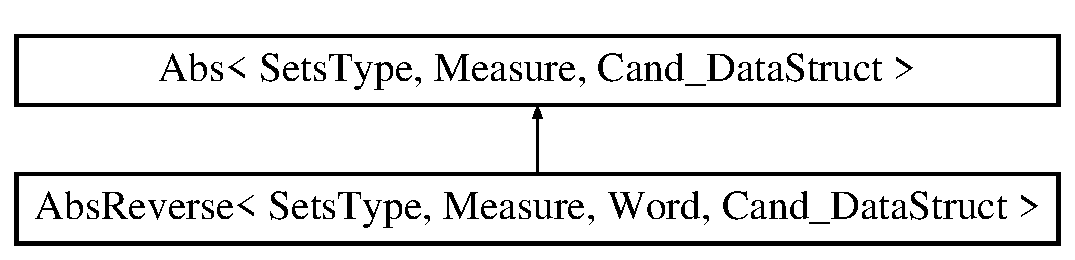
\includegraphics[height=2cm]{class_abs}
\end{center}
\end{figure}
\subsection*{Public Member Functions}
\begin{CompactItemize}
\item 
{\bf Abs} ()\label{class_abs_b9e1bb01229ec95da6b1a5f533dd7151}

\begin{CompactList}\small\item\em Constructor. \item\end{CompactList}\item 
{\bf $\sim$Abs} ()\label{class_abs_72d51b48cb02d0fbb3815d6f8dbf67e6}

\begin{CompactList}\small\item\em Destructor. \item\end{CompactList}\item 
template$<$class Init\-Functor, class Predicate, class Stop\-Iteration, class Output\-Bd\-P, class Output\-Bd\-N, class f$>$ void {\bf operator()} (Init\-Functor \&init, {\bf Predicate} \&pred, Stop\-Iteration $\ast$stop\-Dualization, Output\-Bd\-P $\ast$out\-Bd\-P, Output\-Bd\-N $\ast$out\-Bd\-N, f \&word\-To\-Set)
\begin{CompactList}\small\item\em Functor operator that executes the algorithm. \item\end{CompactList}\item 
template$<$class Init\-Functor, class Predicate, class Stop\-Iteration, class Output\-Bd\-P, class Output\-Bd\-N$>$ void {\bf operator()} (Init\-Functor \&init, {\bf Predicate} \&pred, Stop\-Iteration $\ast$stop\-Dualization, Output\-Bd\-P $\ast$out\-Bd\-P, Output\-Bd\-N $\ast$out\-Bd\-N)
\begin{CompactList}\small\item\em Functor operator that executes the algorithm. \item\end{CompactList}\end{CompactItemize}
\subsection*{Public Attributes}
\begin{CompactItemize}
\item 
bool {\bf verbose}\label{class_abs_346a3f491c7896baa2669113764d9fa7}

\begin{CompactList}\small\item\em {\bf Boolean}{\rm (p.\,\pageref{class_boolean})} to print to screen some informations during the execution (default false). \item\end{CompactList}\end{CompactItemize}
\subsection*{Protected Member Functions}
\begin{CompactItemize}
\item 
template$<$class Init\-Functor, class Predicate, class Stop\-Iteration, class Output\-Bd\-P, class Output\-Bd\-N, class Error, class f$>$ void {\bf execute\-Algorithm} (Init\-Functor \&init, {\bf Predicate} $\ast$pred, Stop\-Iteration $\ast$stop\-Dualization, Output\-Bd\-P $\ast$out\-Bd\-P, Output\-Bd\-N $\ast$out\-Bd\-N, Error $\ast$error, f \&word\-To\-Set)
\begin{CompactList}\small\item\em Execute the algorithm. \item\end{CompactList}\item 
template$<$class Predicate, class Error, class f$>$ int {\bf process\-Opt\-Gen\-Sub} ({\bf Predicate} $\ast$pred, {\bf PTree}$<$ Sets\-Type, Measure $>$ $\ast$compl\-Set, {\bf PTree}$<$ Sets\-Type, Measure $>$ $\ast$opt, {\bf PTree}$<$ Sets\-Type, Measure $>$ $\ast$tr, {\bf PTree}$<$ Sets\-Type, Measure $>$ $\ast$freq\-Tr, {\bf PTree}$<$ Sets\-Type, Measure $>$ $\ast$sub\-Set, int size, f \&word\-To\-Set, Error $\ast$error)
\begin{CompactList}\small\item\em Process the optimist positive border. \item\end{CompactList}\item 
void {\bf move\-Trans\-Freq} (vect\-UI $\ast$itemset, {\bf PTree}$<$ Sets\-Type, Measure $>$ $\ast$tr, {\bf PTree}$<$ Sets\-Type, Measure $>$ $\ast$freq\-Tr)
\begin{CompactList}\small\item\em Method that move a minimal transversal which have \char`\"{}generated\char`\"{} an interesting set from the set of minimal transversals to another set. \item\end{CompactList}\item 
template$<$class Predicate, class f$>$ int {\bf prune\-Candidates} ({\bf Predicate} $\ast$pred, {\bf PTree}$<$ Sets\-Type, Measure $>$ $\ast$tr, int level, deq\-It\-Cand \&last\-Bd\-NElem, f \&word\-To\-Set)
\begin{CompactList}\small\item\em Prune the not interesting elements generated by the levelwise exploration. \item\end{CompactList}\item 
void {\bf gen\-Cand} ({\bf PTree}$<$ Sets\-Type, Measure $>$ $\ast$sub\-Set, {\bf PTree}$<$ Sets\-Type, Measure $>$ $\ast$inbdp)
\begin{CompactList}\small\item\em Method generating the candidates of the levelwise exploration. \item\end{CompactList}\item 
template$<$class Predicate, class f$>$ void {\bf opt\-Approach} ({\bf Predicate} $\ast$pred, set$<$ {\bf PTree}$<$ Sets\-Type, Measure $>$ $>$ $\ast$opt\-It, int lvl, f \&word\-To\-Set)
\begin{CompactList}\small\item\em Method used to do the optimist approach based on \char`\"{}almost interesting\char`\"{} elements. \item\end{CompactList}\item 
template$<$class Predicate, class f$>$ int {\bf prune\-Candidates\-Opt} ({\bf Predicate} $\ast$pred, {\bf PTree}$<$ Sets\-Type, Measure $>$ $\ast$tr, f \&word\-To\-Set)
\begin{CompactList}\small\item\em \char`\"{}Prune\char`\"{} the interesting elements when exploring almost interesting elements. \item\end{CompactList}\end{CompactItemize}
\subsection*{Protected Attributes}
\begin{CompactItemize}
\item 
{\bf Apriori}$<$ Sets\-Type, Measure, Cand\_\-Data\-Struct $>$ {\bf apriori}\label{class_abs_e5143798f9be145d0712d57d553915c2}

\begin{CompactList}\small\item\em Algorithm apriori used for the bottom up initialization. \item\end{CompactList}\item 
Cand\_\-Data\-Struct $\ast$ {\bf bd\-N}\label{class_abs_84861429e931d82ff76926e5709ecd3f}

\begin{CompactList}\small\item\em Negative border. \item\end{CompactList}\item 
Cand\_\-Data\-Struct $\ast$ {\bf bd\-P}\label{class_abs_891257e049d0299337be5a48983a5297}

\begin{CompactList}\small\item\em Positive border. \item\end{CompactList}\end{CompactItemize}


\subsection{Detailed Description}
\subsubsection*{template$<$class Sets\-Type = int, class Measure = Boolean, class Cand\_\-Data\-Struct = PTree$<$Sets\-Type,Measure $>$$>$ class Abs$<$ Sets\-Type, Measure, Cand\_\-Data\-Struct $>$}

Functor finding the negative border Bd- and/or the positive border Bd+ using the algorithm ABS. 

The algorithme (\char`\"{}()\char`\"{} method)take in parameter: the initialisation functor, the predicate, the functor determining at which iteration the levelwise step is stop, the positive and/or negative borders (optional), the transformation function (optional).

The method execute\-Algorithm could be use to execute the algorithm. This method have another parameter to deal with \char`\"{}almost interesting elements\char`\"{} based on an error function passed i n parameter. These elements are considered as interesting during the iterations, and at the end they are used to do a top-down traversal of the search space to find the latests elements of Bd+.

The template parameter Sets\-Type represents the type of the elements of the set representation. The template parameter Measure is the type of the value eventually associated with the word of the language. The template parameter Cand\_\-Data\-Struct is the data structure type used by the algorithms to manipulate the candidates generated. 



\subsection{Member Function Documentation}
\index{Abs@{Abs}!executeAlgorithm@{executeAlgorithm}}
\index{executeAlgorithm@{executeAlgorithm}!Abs@{Abs}}
\subsubsection{\setlength{\rightskip}{0pt plus 5cm}template$<$class Sets\-Type, class Measure, class Cand\_\-Data\-Struct$>$ template$<$class Init\-Functor, class Predicate, class Stop\-Iteration, class Output\-Bd\-P, class Output\-Bd\-N, class Error, class f$>$ void {\bf Abs}$<$ Sets\-Type, Measure, Cand\_\-Data\-Struct $>$::execute\-Algorithm (Init\-Functor \& {\em init}, {\bf Predicate} $\ast$ {\em pred}, Stop\-Iteration $\ast$ {\em stop\-Dualization}, Output\-Bd\-P $\ast$ {\em out\-Bd\-P}, Output\-Bd\-N $\ast$ {\em out\-Bd\-N}, Error $\ast$ {\em error}, f \& {\em word\-To\-Set})\hspace{0.3cm}{\tt  [protected]}}\label{class_abs_33917103181d75de02278cb345c96c1a}


Execute the algorithm. 

\begin{Desc}
\item[Parameters:]
\begin{description}
\item[{\em init}]functor initializing the interesting items wrt predicate. \item[{\em pred}]the predicate \item[{\em stop\-Dualization}]functor determining when the apiori execution must stop \item[{\em bd\-P}]output the positive border in the given objet (must have a push\_\-back( container, measure ) method). \item[{\em bd\-N}]output the negative border in the given objet (must have a push\_\-back( container, measure ) method). \item[{\em error}]function processing if a not interesting element of the optimistic positive border is \char`\"{}almost interesting\char`\"{} \end{description}
\end{Desc}
\index{Abs@{Abs}!genCand@{genCand}}
\index{genCand@{genCand}!Abs@{Abs}}
\subsubsection{\setlength{\rightskip}{0pt plus 5cm}template$<$class Sets\-Type, class Measure, class Cand\_\-Data\-Struct$>$ void {\bf Abs}$<$ Sets\-Type, Measure, Cand\_\-Data\-Struct $>$::gen\-Cand ({\bf PTree}$<$ Sets\-Type, Measure $>$ $\ast$ {\em sub\-Set}, {\bf PTree}$<$ Sets\-Type, Measure $>$ $\ast$ {\em inbdp})\hspace{0.3cm}{\tt  [protected]}}\label{class_abs_41ebb2a6cc990dee19092f6ca21effa8}


Method generating the candidates of the levelwise exploration. 

Actually, this method delete all the subsets generated when processing the optimistic positive border which are included into one element of Bd+.

\begin{Desc}
\item[Parameters:]
\begin{description}
\item[{\em sub\-Set}]subsets of size k+1 of the not interesting elements find in the optimistic positive border. \item[{\em inbdp}]the positive border (all the elements of Bd+ found until the current iteration) \end{description}
\end{Desc}
\index{Abs@{Abs}!moveTransFreq@{moveTransFreq}}
\index{moveTransFreq@{moveTransFreq}!Abs@{Abs}}
\subsubsection{\setlength{\rightskip}{0pt plus 5cm}template$<$class Sets\-Type, class Measure, class Cand\_\-Data\-Struct$>$ void {\bf Abs}$<$ Sets\-Type, Measure, Cand\_\-Data\-Struct $>$::move\-Trans\-Freq (vect\-UI $\ast$ {\em itemset}, {\bf PTree}$<$ Sets\-Type, Measure $>$ $\ast$ {\em tr}, {\bf PTree}$<$ Sets\-Type, Measure $>$ $\ast$ {\em freq\-Tr})\hspace{0.3cm}{\tt  [protected]}}\label{class_abs_4069503604644bb7ddb2404a47098663}


Method that move a minimal transversal which have \char`\"{}generated\char`\"{} an interesting set from the set of minimal transversals to another set. 

\begin{Desc}
\item[Parameters:]
\begin{description}
\item[{\em itemset}]set wich have generated an interesting element \item[{\em tr}]set of the minimal transversals (those which have generated not interesting elements) \item[{\em freq\-Tr}]set of the minmal tranversals which have generated an interesting elements \end{description}
\end{Desc}
\index{Abs@{Abs}!operator()@{operator()}}
\index{operator()@{operator()}!Abs@{Abs}}
\subsubsection{\setlength{\rightskip}{0pt plus 5cm}template$<$class Sets\-Type = int, class Measure = Boolean, class Cand\_\-Data\-Struct = PTree$<$Sets\-Type,Measure $>$$>$ template$<$class Init\-Functor, class Predicate, class Stop\-Iteration, class Output\-Bd\-P, class Output\-Bd\-N$>$ void {\bf Abs}$<$ Sets\-Type, Measure, Cand\_\-Data\-Struct $>$::operator() (Init\-Functor \& {\em init}, {\bf Predicate} \& {\em pred}, Stop\-Iteration $\ast$ {\em stop\-Dualization}, Output\-Bd\-P $\ast$ {\em out\-Bd\-P}, Output\-Bd\-N $\ast$ {\em out\-Bd\-N})\hspace{0.3cm}{\tt  [inline]}}\label{class_abs_1cb8186e971cbb42b54d29bab5ba1e01}


Functor operator that executes the algorithm. 

\begin{Desc}
\item[Parameters:]
\begin{description}
\item[{\em init}]functor initializing the interesting items wrt predicate. \item[{\em pred}]the predicate \item[{\em stop\-Dualization}]functor determining when the apiori execution must stop \item[{\em bd\-P}]output the positive border in the given objet (must have a push\_\-back( container, measure ) method). \item[{\em bd\-N}]output the negative border in the given objet (must have a push\_\-back( container, measure ) method). \end{description}
\end{Desc}


Reimplemented in {\bf Abs\-Reverse$<$ Sets\-Type, Measure, Word, Cand\_\-Data\-Struct $>$} {\rm (p.\,\pageref{class_abs_reverse_783d932854ce93bd14518406996d8090})}.\index{Abs@{Abs}!operator()@{operator()}}
\index{operator()@{operator()}!Abs@{Abs}}
\subsubsection{\setlength{\rightskip}{0pt plus 5cm}template$<$class Sets\-Type = int, class Measure = Boolean, class Cand\_\-Data\-Struct = PTree$<$Sets\-Type,Measure $>$$>$ template$<$class Init\-Functor, class Predicate, class Stop\-Iteration, class Output\-Bd\-P, class Output\-Bd\-N, class f$>$ void {\bf Abs}$<$ Sets\-Type, Measure, Cand\_\-Data\-Struct $>$::operator() (Init\-Functor \& {\em init}, {\bf Predicate} \& {\em pred}, Stop\-Iteration $\ast$ {\em stop\-Dualization}, Output\-Bd\-P $\ast$ {\em out\-Bd\-P}, Output\-Bd\-N $\ast$ {\em out\-Bd\-N}, f \& {\em word\-To\-Set})\hspace{0.3cm}{\tt  [inline]}}\label{class_abs_991fe73b7db6f50b75e434631187ec9a}


Functor operator that executes the algorithm. 

\begin{Desc}
\item[Parameters:]
\begin{description}
\item[{\em init}]functor initializing the interesting items wrt predicate \item[{\em pred}]the predicate \item[{\em stop\-Dualization}]functor determining when the apiori execution must stop \item[{\em bd\-P}]output the positive border in the given objet (must have a push\_\-back( container, measure ) method). \item[{\em bd\-N}]output the negative border in the given objet (must have a push\_\-back( container, measure ) method). \item[{\em word\-Toset}]transformation function \end{description}
\end{Desc}


Reimplemented in {\bf Abs\-Reverse$<$ Sets\-Type, Measure, Word, Cand\_\-Data\-Struct $>$} {\rm (p.\,\pageref{class_abs_reverse_d4e6aa7d0f2e50db5d5e75ab5801fd51})}.\index{Abs@{Abs}!optApproach@{optApproach}}
\index{optApproach@{optApproach}!Abs@{Abs}}
\subsubsection{\setlength{\rightskip}{0pt plus 5cm}template$<$class Sets\-Type, class Measure, class Cand\_\-Data\-Struct$>$ template$<$class Predicate, class f$>$ void {\bf Abs}$<$ Sets\-Type, Measure, Cand\_\-Data\-Struct $>$::opt\-Approach ({\bf Predicate} $\ast$ {\em pred}, set$<$ {\bf PTree}$<$ Sets\-Type, Measure $>$ $>$ $\ast$ {\em opt\-It}, int {\em lvl}, f \& {\em word\-To\-Set})\hspace{0.3cm}{\tt  [protected]}}\label{class_abs_61298c6d5b7e4ff5192b2a68c52b701a}


Method used to do the optimist approach based on \char`\"{}almost interesting\char`\"{} elements. 

From a set of sets in parameter, it founds all the maximals interesting sets of the sub lattice until a given level. the exploration of the search space id done level by level.

\begin{Desc}
\item[Parameters:]
\begin{description}
\item[{\em pred}]the predicate \item[{\em opt\-It}]set containing the almost interesting elements (strored by size) \item[{\em lvl}]the \char`\"{}smallest\char`\"{} level to explore \item[{\em word\-Toset}]transformation function \end{description}
\end{Desc}
\index{Abs@{Abs}!processOptGenSub@{processOptGenSub}}
\index{processOptGenSub@{processOptGenSub}!Abs@{Abs}}
\subsubsection{\setlength{\rightskip}{0pt plus 5cm}template$<$class Sets\-Type, class Measure, class Cand\_\-Data\-Struct$>$ template$<$class Predicate, class Error, class f$>$ int {\bf Abs}$<$ Sets\-Type, Measure, Cand\_\-Data\-Struct $>$::process\-Opt\-Gen\-Sub ({\bf Predicate} $\ast$ {\em pred}, {\bf PTree}$<$ Sets\-Type, Measure $>$ $\ast$ {\em compl\-Set}, {\bf PTree}$<$ Sets\-Type, Measure $>$ $\ast$ {\em opt}, {\bf PTree}$<$ Sets\-Type, Measure $>$ $\ast$ {\em tr}, {\bf PTree}$<$ Sets\-Type, Measure $>$ $\ast$ {\em freq\-Tr}, {\bf PTree}$<$ Sets\-Type, Measure $>$ $\ast$ {\em sub\-Set}, int {\em size}, f \& {\em word\-To\-Set}, Error $\ast$ {\em error})\hspace{0.3cm}{\tt  [protected]}}\label{class_abs_18e3c9003dca0c22177631287ce60aa5}


Process the optimist positive border. 

All the interesting sets update Bd+ and the subests of the not interesting sets are generated. If the \char`\"{}almost interesting\char`\"{} elements are studied, this method save these elements in a particular data structure. To optimize the minimal transversal computation, minimal transversals which have generated an interesting element are stored separately.

\begin{Desc}
\item[Parameters:]
\begin{description}
\item[{\em pred}]the predicate \item[{\em compl\-Set}]set of complements of the minimal transversals in the current iteration \item[{\em opt}]set used to store the almost interesting elments (not necessarly used) \item[{\em tr}]set of the minimal transversals find until the current iteration \item[{\em freqtr}]set of the minimal transversals find until the current iteration and which have generated an interesting element \item[{\em sub\-Set}]strore the subsets of size k (current level of the levelwise approach) of the not interesting elements fond in the optimistic positive border \item[{\em size}]current level of the levelwise approach \item[{\em word\-Toset}]transformation function \item[{\em error}]function processing if a not interesting element of the optimistic positive border is \char`\"{}almost interesting\char`\"{} \end{description}
\end{Desc}
\index{Abs@{Abs}!pruneCandidates@{pruneCandidates}}
\index{pruneCandidates@{pruneCandidates}!Abs@{Abs}}
\subsubsection{\setlength{\rightskip}{0pt plus 5cm}template$<$class Sets\-Type, class Measure, class Cand\_\-Data\-Struct$>$ template$<$class Predicate, class f$>$ int {\bf Abs}$<$ Sets\-Type, Measure, Cand\_\-Data\-Struct $>$::prune\-Candidates ({\bf Predicate} $\ast$ {\em pred}, {\bf PTree}$<$ Sets\-Type, Measure $>$ $\ast$ {\em tr}, int {\em level}, deq\-It\-Cand \& {\em last\-Bd\-NElem}, f \& {\em word\-To\-Set})\hspace{0.3cm}{\tt  [protected]}}\label{class_abs_46ecf54530c316a639b3533386af9d4b}


Prune the not interesting elements generated by the levelwise exploration. 

\begin{Desc}
\item[Parameters:]
\begin{description}
\item[{\em pred}]the predicate \item[{\em tr}]set of the candidates generated by the levelwise exploration \item[{\em level}]current level of the levelwise exploration \item[{\em last\-Bd\-NElem}]elements (iterators on) of the negative border found in the current iteration \item[{\em word\-Toset}]transformation function \end{description}
\end{Desc}
\index{Abs@{Abs}!pruneCandidatesOpt@{pruneCandidatesOpt}}
\index{pruneCandidatesOpt@{pruneCandidatesOpt}!Abs@{Abs}}
\subsubsection{\setlength{\rightskip}{0pt plus 5cm}template$<$class Sets\-Type, class Measure, class Cand\_\-Data\-Struct$>$ template$<$class Predicate, class f$>$ int {\bf Abs}$<$ Sets\-Type, Measure, Cand\_\-Data\-Struct $>$::prune\-Candidates\-Opt ({\bf Predicate} $\ast$ {\em pred}, {\bf PTree}$<$ Sets\-Type, Measure $>$ $\ast$ {\em tr}, f \& {\em word\-To\-Set})\hspace{0.3cm}{\tt  [protected]}}\label{class_abs_9756459bbd5a86de592167e310c576fa}


\char`\"{}Prune\char`\"{} the interesting elements when exploring almost interesting elements. 

The interesting elements are pruned for further exploration but stored in the positive border.

\begin{Desc}
\item[Parameters:]
\begin{description}
\item[{\em pred}]the predicate \item[{\em tr}]the set of candidates generated by the exploration \item[{\em word\-Toset}]transformation function \end{description}
\end{Desc}


The documentation for this class was generated from the following file:\begin{CompactItemize}
\item 
F:/i\-Zi/algorithms/Abs.hxx\end{CompactItemize}

\section{Abs\-Reverse$<$ Sets\-Type, Measure, Word, Cand\_\-Data\-Struct $>$ Class Template Reference}
\label{class_abs_reverse}\index{AbsReverse@{AbsReverse}}
Functor finding the negative border Bd- and/or the positive border Bd+ using the algorithm ABS doing a top dow exploration of the search space.  


{\tt \#include $<$Abs\-Reverse.hxx$>$}

Inheritance diagram for Abs\-Reverse$<$ Sets\-Type, Measure, Word, Cand\_\-Data\-Struct $>$::\begin{figure}[H]
\begin{center}
\leavevmode
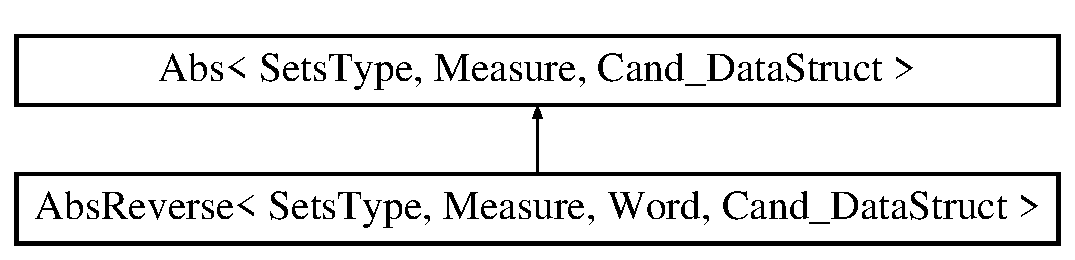
\includegraphics[height=2cm]{class_abs_reverse}
\end{center}
\end{figure}
\subsection*{Public Member Functions}
\begin{CompactItemize}
\item 
{\bf Abs\-Reverse} ()\label{class_abs_reverse_800fd75345935e7c59ee5058be8c4b1c}

\begin{CompactList}\small\item\em Constructor. \item\end{CompactList}\item 
{\bf $\sim$Abs\-Reverse} ()\label{class_abs_reverse_5a78f7a72b09b62b6e5326931890deef}

\begin{CompactList}\small\item\em Destructor. \item\end{CompactList}\item 
template$<$class Init\-Functor, class Predicate, class Stop\-Iteration, class Output\-Bd\-P, class Output\-Bd\-N, class f$>$ void {\bf operator()} (Init\-Functor \&init, {\bf Predicate} \&pred, Stop\-Iteration $\ast$stop\-Dualization, Output\-Bd\-P $\ast$out\-Bd\-P, Output\-Bd\-N $\ast$out\-Bd\-N, f \&word\-To\-Set)
\begin{CompactList}\small\item\em Functor operator that executes the algorithm. \item\end{CompactList}\item 
template$<$class Init\-Functor, class Predicate, class Stop\-Iteration, class Output\-Bd\-P, class Output\-Bd\-N$>$ void {\bf operator()} (Init\-Functor \&init, {\bf Predicate} \&pred, Stop\-Iteration $\ast$stop\-Dualization, Output\-Bd\-P $\ast$out\-Bd\-P, Output\-Bd\-N $\ast$out\-Bd\-N)
\begin{CompactList}\small\item\em Functor operator that executes the algorithm. \item\end{CompactList}\end{CompactItemize}


\subsection{Detailed Description}
\subsubsection*{template$<$class Sets\-Type = int, class Measure = Boolean, class Word = vector$<$ Sets\-Type $>$, class Cand\_\-Data\-Struct = PTree$<$Sets\-Type,Measure $>$$>$ class Abs\-Reverse$<$ Sets\-Type, Measure, Word, Cand\_\-Data\-Struct $>$}

Functor finding the negative border Bd- and/or the positive border Bd+ using the algorithm ABS doing a top dow exploration of the search space. 

The algorithme (\char`\"{}()\char`\"{} method)take in parameter: the initialisation functor, the predicate, the functor determining at which iteration the levelwise step is stop, the positive and/or negative borders (optional), the transformation function (optional).

The method execute\-Algorithm could be use to execute the algorithm. This method have another parameter to deal with \char`\"{}almost interesting elements\char`\"{} based on an error function passed i n parameter. These elements are considered as interesting during the iterations, and at the end they are used to do a top-down traversal of the search space to find the latests elements of Bd+.

The template parameter Sets\-Type represents the type of the elements of the set representation. The template parameter Measure is the type of the value eventually associated with the word of the language. The template parameter Word represents the type of the elements of the language. The template parameter Cand\_\-Data\-Struct is the data structure type used by the algorithms to manipulate the candidates generated. 



\subsection{Member Function Documentation}
\index{AbsReverse@{Abs\-Reverse}!operator()@{operator()}}
\index{operator()@{operator()}!AbsReverse@{Abs\-Reverse}}
\subsubsection{\setlength{\rightskip}{0pt plus 5cm}template$<$class Sets\-Type = int, class Measure = Boolean, class Word = vector$<$ Sets\-Type $>$, class Cand\_\-Data\-Struct = PTree$<$Sets\-Type,Measure $>$$>$ template$<$class Init\-Functor, class Predicate, class Stop\-Iteration, class Output\-Bd\-P, class Output\-Bd\-N$>$ void {\bf Abs\-Reverse}$<$ Sets\-Type, Measure, Word, Cand\_\-Data\-Struct $>$::operator() (Init\-Functor \& {\em init}, {\bf Predicate} \& {\em pred}, Stop\-Iteration $\ast$ {\em stop\-Dualization}, Output\-Bd\-P $\ast$ {\em out\-Bd\-P}, Output\-Bd\-N $\ast$ {\em out\-Bd\-N})\hspace{0.3cm}{\tt  [inline]}}\label{class_abs_reverse_783d932854ce93bd14518406996d8090}


Functor operator that executes the algorithm. 

\begin{Desc}
\item[Parameters:]
\begin{description}
\item[{\em init}]functor initializing the interesting items wrt predicate. \item[{\em pred}]the predicate \item[{\em stop\-Dualization}]functor determining when the apiori execution must stop \item[{\em bd\-P}]output the positive border in the given objet (must have a push\_\-back( container, measure ) method). \item[{\em bd\-N}]output the negative border in the given objet (must have a push\_\-back( container, measure ) method). \end{description}
\end{Desc}


Reimplemented from {\bf Abs$<$ Sets\-Type, Measure, Cand\_\-Data\-Struct $>$} {\rm (p.\,\pageref{class_abs_1cb8186e971cbb42b54d29bab5ba1e01})}.\index{AbsReverse@{Abs\-Reverse}!operator()@{operator()}}
\index{operator()@{operator()}!AbsReverse@{Abs\-Reverse}}
\subsubsection{\setlength{\rightskip}{0pt plus 5cm}template$<$class Sets\-Type = int, class Measure = Boolean, class Word = vector$<$ Sets\-Type $>$, class Cand\_\-Data\-Struct = PTree$<$Sets\-Type,Measure $>$$>$ template$<$class Init\-Functor, class Predicate, class Stop\-Iteration, class Output\-Bd\-P, class Output\-Bd\-N, class f$>$ void {\bf Abs\-Reverse}$<$ Sets\-Type, Measure, Word, Cand\_\-Data\-Struct $>$::operator() (Init\-Functor \& {\em init}, {\bf Predicate} \& {\em pred}, Stop\-Iteration $\ast$ {\em stop\-Dualization}, Output\-Bd\-P $\ast$ {\em out\-Bd\-P}, Output\-Bd\-N $\ast$ {\em out\-Bd\-N}, f \& {\em word\-To\-Set})\hspace{0.3cm}{\tt  [inline]}}\label{class_abs_reverse_d4e6aa7d0f2e50db5d5e75ab5801fd51}


Functor operator that executes the algorithm. 

\begin{Desc}
\item[Parameters:]
\begin{description}
\item[{\em init}]functor initializing the interesting items wrt predicate \item[{\em pred}]the predicate \item[{\em stop\-Dualization}]functor determining when the apiori execution must stop \item[{\em bd\-P}]output the positive border in the given objet (must have a push\_\-back( container, measure ) method). \item[{\em bd\-N}]output the negative border in the given objet (must have a push\_\-back( container, measure ) method). \item[{\em word\-Toset}]transformation function \end{description}
\end{Desc}


Reimplemented from {\bf Abs$<$ Sets\-Type, Measure, Cand\_\-Data\-Struct $>$} {\rm (p.\,\pageref{class_abs_991fe73b7db6f50b75e434631187ec9a})}.

The documentation for this class was generated from the following file:\begin{CompactItemize}
\item 
F:/i\-Zi/algorithms/Abs\-Reverse.hxx\end{CompactItemize}

\section{Apriori$<$ Sets\-Type, Measure, Cand\_\-Data\-Struct $>$ Class Template Reference}
\label{class_apriori}\index{Apriori@{Apriori}}
Functor finding the theory and/or the negative border and/or the positive border using the algorithm {\bf Apriori}{\rm (p.\,\pageref{class_apriori})}.  


{\tt \#include $<$Apriori.hxx$>$}

Inheritance diagram for Apriori$<$ Sets\-Type, Measure, Cand\_\-Data\-Struct $>$::\begin{figure}[H]
\begin{center}
\leavevmode
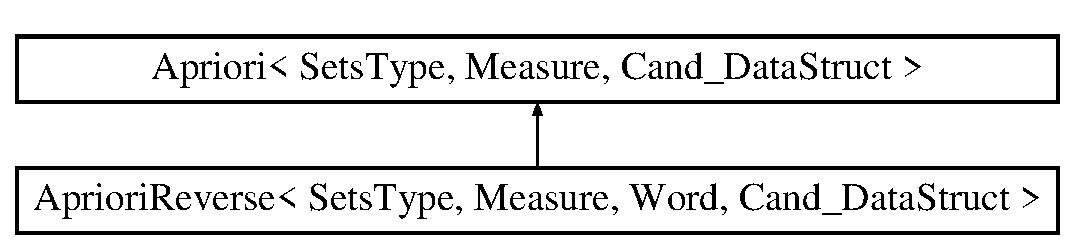
\includegraphics[height=2cm]{class_apriori}
\end{center}
\end{figure}
\subsection*{Public Member Functions}
\begin{CompactItemize}
\item 
template$<$class Init\-Functor, class Predicate, class Output\-Theory, class Output\-Bd\-P, class Output\-Bd\-N, class f, class Stop\-Iteration, class f2$>$ void {\bf execute\-Algo} (Init\-Functor \&init, {\bf Predicate} $\ast$pred, Output\-Theory $\ast$theory, Output\-Bd\-P $\ast$bd\-P, Output\-Bd\-N $\ast$bd\-N, f \&word\-To\-Set, Stop\-Iteration $\ast$stop\-Ite, f2 \&word\-To\-Set\-Save, deque$<$ Sets\-Type $>$ $\ast$list\-Interes\-Items=0)
\begin{CompactList}\small\item\em Function that execute the algorithm operator that executes the algorithm. \item\end{CompactList}\item 
{\bf Apriori} ()\label{class_apriori_8287a89c0b7f56a814f945e75ca29f0d}

\begin{CompactList}\small\item\em Constructor. \item\end{CompactList}\item 
template$<$class Init\-Functor, class Predicate, class Output\-Theory, class Output\-Bd\-P, class Output\-Bd\-N, class f$>$ void {\bf operator()} (Init\-Functor \&init, {\bf Predicate} \&pred, Output\-Theory $\ast$theory, Output\-Bd\-P $\ast$bd\-P, Output\-Bd\-N $\ast$bd\-N, f \&word\-To\-Set)
\begin{CompactList}\small\item\em Functor operator that executes the algorithm. \item\end{CompactList}\item 
template$<$class Init\-Functor, class Predicate, class Output\-Theory, class Output\-Bd\-P, class Output\-Bd\-N$>$ void {\bf operator()} (Init\-Functor \&init, {\bf Predicate} \&pred, Output\-Theory $\ast$theory, Output\-Bd\-P $\ast$bd\-P, Output\-Bd\-N $\ast$bd\-N)
\begin{CompactList}\small\item\em Functor operator that executes the algorithm. \item\end{CompactList}\item 
template$<$class Init\-Functor, class Predicate, class Output\-Theory, class Output\-Bd\-P, class Output\-Bd\-N, class f, class Stop\-Iteration$>$ void {\bf operator()} (Init\-Functor \&init, {\bf Predicate} \&pred, Output\-Theory $\ast$theory, Output\-Bd\-P $\ast$bd\-P, Output\-Bd\-N $\ast$bd\-N, Stop\-Iteration $\ast$stop\-Ite, f \&word\-To\-Set)
\begin{CompactList}\small\item\em Functor operator that executes the algorithm and stop his execution when the functor passed in parameter return false. \item\end{CompactList}\item 
template$<$class Init\-Functor, class Predicate, class Output\-Theory, class Output\-Bd\-P, class Output\-Bd\-N, class Stop\-Iteration$>$ void {\bf operator()} (Init\-Functor \&init, {\bf Predicate} \&pred, Output\-Theory $\ast$theory, Output\-Bd\-P $\ast$bd\-P, Output\-Bd\-N $\ast$bd\-N, Stop\-Iteration $\ast$stop\-Ite)
\begin{CompactList}\small\item\em Functor operator that executes the algorithm and stop his execution when the functor passed in parameter return false. \item\end{CompactList}\end{CompactItemize}
\subsection*{Public Attributes}
\begin{CompactItemize}
\item 
bool {\bf verbose}\label{class_apriori_de33c80face437efdf4b032849811d07}

\begin{CompactList}\small\item\em {\bf Boolean}{\rm (p.\,\pageref{class_boolean})} to print to screen some informations during the execution (default false). \item\end{CompactList}\item 
bool {\bf save\-Set}\label{class_apriori_7fd142ed119cef31fdcb325709425ab6}

\begin{CompactList}\small\item\em {\bf Boolean}{\rm (p.\,\pageref{class_boolean})} to save the set representation of the solution. \item\end{CompactList}\end{CompactItemize}
\subsection*{Protected Member Functions}
\begin{CompactItemize}
\item 
template$<$class Iterator$>$ bool {\bf test\-Subset} (Iterator \&it\-Pref, Iterator \&it\-Last, vector$<$ Sets\-Type $>$ \&buffer)
\begin{CompactList}\small\item\em Test if a set generated using the elements pointed by it\-Pref and it\-Last is a candidate. \item\end{CompactList}\item 
template$<$class Iterator$>$ void {\bf erase\-Subset} (Cand\_\-Data\-Struct \&cand, Iterator \&position, vector$<$ Sets\-Type $>$ \&buffer)
\begin{CompactList}\small\item\em Erase all the k-1 subsets of the set of size k coresponding to the iterator in parameter. \item\end{CompactList}\item 
void {\bf filter} (Cand\_\-Data\-Struct \&cand)
\begin{CompactList}\small\item\em Filter the elements of the positive border from the theory. \item\end{CompactList}\item 
int {\bf candidates\-Generation} (Cand\_\-Data\-Struct \&cand, int \&level)
\begin{CompactList}\small\item\em Candidate generation phase of {\bf Apriori}{\rm (p.\,\pageref{class_apriori})}. \item\end{CompactList}\item 
template$<$class Predicate, class Output\-Theory, class Output\-Bd\-N, class f, class f2$>$ int {\bf prune} (Cand\_\-Data\-Struct \&cand, {\bf Predicate} $\ast$pred, Output\-Theory $\ast$theory, Output\-Bd\-N $\ast$bd\-N, f \&word\-To\-Set, f2 \&word\-To\-Set\-Save, deque$<$ Sets\-Type $>$ $\ast$list\-Interes\-Items=0)
\begin{CompactList}\small\item\em Pruning generation phase of {\bf Apriori}{\rm (p.\,\pageref{class_apriori})}. \item\end{CompactList}\end{CompactItemize}
\subsection*{Protected Attributes}
\begin{CompactItemize}
\item 
Cand\_\-Data\-Struct {\bf candidates}\label{class_apriori_7a7457c2cb4aacb56a88c1f70bfa5b88}

\begin{CompactList}\small\item\em The candidates generated. \item\end{CompactList}\end{CompactItemize}
\subsection*{Classes}
\begin{CompactItemize}
\item 
class {\bf init\-Candidates}
\begin{CompactList}\small\item\em Initialize the set of candidates with the basic words of the language. \item\end{CompactList}\end{CompactItemize}


\subsection{Detailed Description}
\subsubsection*{template$<$class Sets\-Type = int, class Measure = Boolean, class Cand\_\-Data\-Struct = PTree$<$Sets\-Type,Measure$>$$>$ class Apriori$<$ Sets\-Type, Measure, Cand\_\-Data\-Struct $>$}

Functor finding the theory and/or the negative border and/or the positive border using the algorithm {\bf Apriori}{\rm (p.\,\pageref{class_apriori})}. 

This class enables the execution of the classic {\bf Apriori}{\rm (p.\,\pageref{class_apriori})} algorithm. Moreover this class enables to stop the execution of {\bf Apriori}{\rm (p.\,\pageref{class_apriori})} at an iteration wrt to a user defined functor. The template parameter Sets\-Type represents the type of the sets representing the elements of the language. The template parameter Measure is the type of the value eventually associated with the word of the language. The template parameter Cand\_\-Data\-Struct is the data structure type used to store the candidates generated by the algorithms. 



\subsection{Member Function Documentation}
\index{Apriori@{Apriori}!candidatesGeneration@{candidatesGeneration}}
\index{candidatesGeneration@{candidatesGeneration}!Apriori@{Apriori}}
\subsubsection{\setlength{\rightskip}{0pt plus 5cm}template$<$class Sets\-Type, class Measure, class Cand\_\-Data\-Struct$>$ int {\bf Apriori}$<$ Sets\-Type, Measure, Cand\_\-Data\-Struct $>$::candidates\-Generation (Cand\_\-Data\-Struct \& {\em cand}, int \& {\em level})\hspace{0.3cm}{\tt  [protected]}}\label{class_apriori_f7d6a2dbd1c203246f36081ca1f0e325}


Candidate generation phase of {\bf Apriori}{\rm (p.\,\pageref{class_apriori})}. 

\begin{Desc}
\item[Parameters:]
\begin{description}
\item[{\em cand}]set of candidates. \item[{\em level}]current size of the candidates \end{description}
\end{Desc}
\begin{Desc}
\item[Returns:]the number of sets generated. \end{Desc}
\index{Apriori@{Apriori}!eraseSubset@{eraseSubset}}
\index{eraseSubset@{eraseSubset}!Apriori@{Apriori}}
\subsubsection{\setlength{\rightskip}{0pt plus 5cm}template$<$class Sets\-Type, class Measure, class Cand\_\-Data\-Struct$>$ template$<$class Iterator$>$ void {\bf Apriori}$<$ Sets\-Type, Measure, Cand\_\-Data\-Struct $>$::erase\-Subset (Cand\_\-Data\-Struct \& {\em cand}, Iterator \& {\em position}, vector$<$ Sets\-Type $>$ \& {\em buffer})\hspace{0.3cm}{\tt  [protected]}}\label{class_apriori_ea2d007414bb3735d61a1b27a2b14667}


Erase all the k-1 subsets of the set of size k coresponding to the iterator in parameter. 

\begin{Desc}
\item[Parameters:]
\begin{description}
\item[{\em cand}]contains the theory. \item[{\em position}]iterator on the set. \item[{\em buffer}]container of size k used to test subset. \end{description}
\end{Desc}
\index{Apriori@{Apriori}!executeAlgo@{executeAlgo}}
\index{executeAlgo@{executeAlgo}!Apriori@{Apriori}}
\subsubsection{\setlength{\rightskip}{0pt plus 5cm}template$<$class Sets\-Type, class Measure, class Cand\_\-Data\-Struct$>$ template$<$class Init\-Functor, class Predicate, class Output\-Theory, class Output\-Bd\-P, class Output\-Bd\-N, class f, class Stop\-Iteration, class f2$>$ void {\bf Apriori}$<$ Sets\-Type, Measure, Cand\_\-Data\-Struct $>$::execute\-Algo (Init\-Functor \& {\em init}, {\bf Predicate} $\ast$ {\em pred}, Output\-Theory $\ast$ {\em theory}, Output\-Bd\-P $\ast$ {\em bd\-P}, Output\-Bd\-N $\ast$ {\em bd\-N}, f \& {\em word\-To\-Set}, Stop\-Iteration $\ast$ {\em stop\-Ite}, f2 \& {\em word\-To\-Set\-Save}, deque$<$ Sets\-Type $>$ $\ast$ {\em list\-Interes\-Items} = {\tt 0})}\label{class_apriori_cef957e8ca48064546d3aed66c1927c7}


Function that execute the algorithm operator that executes the algorithm. 

\begin{Desc}
\item[Parameters:]
\begin{description}
\item[{\em init}]functor initializing the interesting items wrt predicate. \item[{\em pred}]the predicate \item[{\em theory}]output the theory in the given objet (must have a push\_\-back( container, measure ) method). \item[{\em bd\-P}]output the positive border in the given objet (must have a push\_\-back( container, measure ) method). \item[{\em bd\-N}]output the negative border in the given objet (must have a push\_\-back( container, measure ) method). \item[{\em set\-To\-Word}]transform words of the language studied in sets. \item[{\em stop\-Ite}]functor stop that stop the execution of apriori before the end. \item[{\em set\-To\-Word\-Save}]transform for output the sets find by the algorithm in words of the language. \item[{\em list\-Interest\-Items}]list of all the interesting items (set representation). \end{description}
\end{Desc}
\index{Apriori@{Apriori}!filter@{filter}}
\index{filter@{filter}!Apriori@{Apriori}}
\subsubsection{\setlength{\rightskip}{0pt plus 5cm}template$<$class Sets\-Type, class Measure, class Cand\_\-Data\-Struct$>$ void {\bf Apriori}$<$ Sets\-Type, Measure, Cand\_\-Data\-Struct $>$::filter (Cand\_\-Data\-Struct \& {\em cand})\hspace{0.3cm}{\tt  [protected]}}\label{class_apriori_44e415598f2de8a80b341c53dce01b12}


Filter the elements of the positive border from the theory. 

\begin{Desc}
\item[Parameters:]
\begin{description}
\item[{\em cand}]contains the theory. \end{description}
\end{Desc}
\index{Apriori@{Apriori}!operator()@{operator()}}
\index{operator()@{operator()}!Apriori@{Apriori}}
\subsubsection{\setlength{\rightskip}{0pt plus 5cm}template$<$class Sets\-Type = int, class Measure = Boolean, class Cand\_\-Data\-Struct = PTree$<$Sets\-Type,Measure$>$$>$ template$<$class Init\-Functor, class Predicate, class Output\-Theory, class Output\-Bd\-P, class Output\-Bd\-N, class Stop\-Iteration$>$ void {\bf Apriori}$<$ Sets\-Type, Measure, Cand\_\-Data\-Struct $>$::operator() (Init\-Functor \& {\em init}, {\bf Predicate} \& {\em pred}, Output\-Theory $\ast$ {\em theory}, Output\-Bd\-P $\ast$ {\em bd\-P}, Output\-Bd\-N $\ast$ {\em bd\-N}, Stop\-Iteration $\ast$ {\em stop\-Ite})\hspace{0.3cm}{\tt  [inline]}}\label{class_apriori_117edc08779546395973171927fb8a77}


Functor operator that executes the algorithm and stop his execution when the functor passed in parameter return false. 

\begin{Desc}
\item[Parameters:]
\begin{description}
\item[{\em init}]functor initializing the interesting items wrt predicate. \item[{\em pred}]the predicate \item[{\em theory}]output the theory in the given objet (must have a push\_\-back( container, measure ) method). \item[{\em bd\-P}]output the positive border in the given objet (must have a push\_\-back( container, measure ) method). \item[{\em bd\-N}]output the negative border in the given objet (must have a push\_\-back( container, measure ) method). \item[{\em stop\-Ite}]functor stop that stop the execution of apriori before the end. \item[{\em word\-To\-Set}]transform words of the language studied in sets. \end{description}
\end{Desc}


Reimplemented in {\bf Apriori\-Reverse$<$ Sets\-Type, Measure, Word, Cand\_\-Data\-Struct $>$} {\rm (p.\,\pageref{class_apriori_reverse_a8018f226acaaa0047cf1386ed189e08})}.\index{Apriori@{Apriori}!operator()@{operator()}}
\index{operator()@{operator()}!Apriori@{Apriori}}
\subsubsection{\setlength{\rightskip}{0pt plus 5cm}template$<$class Sets\-Type = int, class Measure = Boolean, class Cand\_\-Data\-Struct = PTree$<$Sets\-Type,Measure$>$$>$ template$<$class Init\-Functor, class Predicate, class Output\-Theory, class Output\-Bd\-P, class Output\-Bd\-N, class f, class Stop\-Iteration$>$ void {\bf Apriori}$<$ Sets\-Type, Measure, Cand\_\-Data\-Struct $>$::operator() (Init\-Functor \& {\em init}, {\bf Predicate} \& {\em pred}, Output\-Theory $\ast$ {\em theory}, Output\-Bd\-P $\ast$ {\em bd\-P}, Output\-Bd\-N $\ast$ {\em bd\-N}, Stop\-Iteration $\ast$ {\em stop\-Ite}, f \& {\em word\-To\-Set})\hspace{0.3cm}{\tt  [inline]}}\label{class_apriori_4ccc3fe5ae7ecaa9efffcdc41d1888ed}


Functor operator that executes the algorithm and stop his execution when the functor passed in parameter return false. 

\begin{Desc}
\item[Parameters:]
\begin{description}
\item[{\em init}]functor initializing the interesting items wrt predicate. \item[{\em pred}]the predicate \item[{\em theory}]output the theory in the given objet (must have a push\_\-back( container, measure ) method). \item[{\em bd\-P}]output the positive border in the given objet (must have a push\_\-back( container, measure ) method). \item[{\em bd\-N}]output the negative border in the given objet (must have a push\_\-back( container, measure ) method). \item[{\em stop\-Ite}]functor stop that stop the execution of apriori before the end. \item[{\em word\-To\-Set}]transform words of the language studied in sets. \end{description}
\end{Desc}


Reimplemented in {\bf Apriori\-Reverse$<$ Sets\-Type, Measure, Word, Cand\_\-Data\-Struct $>$} {\rm (p.\,\pageref{class_apriori_reverse_d898f211e89442230c64651031388e3d})}.\index{Apriori@{Apriori}!operator()@{operator()}}
\index{operator()@{operator()}!Apriori@{Apriori}}
\subsubsection{\setlength{\rightskip}{0pt plus 5cm}template$<$class Sets\-Type = int, class Measure = Boolean, class Cand\_\-Data\-Struct = PTree$<$Sets\-Type,Measure$>$$>$ template$<$class Init\-Functor, class Predicate, class Output\-Theory, class Output\-Bd\-P, class Output\-Bd\-N$>$ void {\bf Apriori}$<$ Sets\-Type, Measure, Cand\_\-Data\-Struct $>$::operator() (Init\-Functor \& {\em init}, {\bf Predicate} \& {\em pred}, Output\-Theory $\ast$ {\em theory}, Output\-Bd\-P $\ast$ {\em bd\-P}, Output\-Bd\-N $\ast$ {\em bd\-N})\hspace{0.3cm}{\tt  [inline]}}\label{class_apriori_f0a2087314d1753cc3dd397c4a3f3dda}


Functor operator that executes the algorithm. 

\begin{Desc}
\item[Parameters:]
\begin{description}
\item[{\em init}]functor initializing the interesting items wrt predicate. \item[{\em pred}]the predicate \item[{\em theory}]output the theory in the given objet (must have a push\_\-back( container, measure ) method). \item[{\em bd\-P}]output the positive border in the given objet (must have a push\_\-back( container, measure ) method). \item[{\em bd\-N}]output the negative border in the given objet (must have a push\_\-back( container, measure ) method). \end{description}
\end{Desc}


Reimplemented in {\bf Apriori\-Reverse$<$ Sets\-Type, Measure, Word, Cand\_\-Data\-Struct $>$} {\rm (p.\,\pageref{class_apriori_reverse_5266cde8d5a9455c9f9281e435754ca9})}.\index{Apriori@{Apriori}!operator()@{operator()}}
\index{operator()@{operator()}!Apriori@{Apriori}}
\subsubsection{\setlength{\rightskip}{0pt plus 5cm}template$<$class Sets\-Type = int, class Measure = Boolean, class Cand\_\-Data\-Struct = PTree$<$Sets\-Type,Measure$>$$>$ template$<$class Init\-Functor, class Predicate, class Output\-Theory, class Output\-Bd\-P, class Output\-Bd\-N, class f$>$ void {\bf Apriori}$<$ Sets\-Type, Measure, Cand\_\-Data\-Struct $>$::operator() (Init\-Functor \& {\em init}, {\bf Predicate} \& {\em pred}, Output\-Theory $\ast$ {\em theory}, Output\-Bd\-P $\ast$ {\em bd\-P}, Output\-Bd\-N $\ast$ {\em bd\-N}, f \& {\em word\-To\-Set})\hspace{0.3cm}{\tt  [inline]}}\label{class_apriori_36d7a2cdad2a8c459f2b44e3ab460591}


Functor operator that executes the algorithm. 

\begin{Desc}
\item[Parameters:]
\begin{description}
\item[{\em init}]functor initializing the interesting items wrt predicate. \item[{\em pred}]the predicate \item[{\em theory}]output the theory in the given objet (must have a push\_\-back( container, measure ) method). \item[{\em bd\-P}]output the positive border in the given objet (must have a push\_\-back( container, measure ) method). \item[{\em bd\-N}]output the negative border in the given objet (must have a push\_\-back( container, measure ) method). \item[{\em word\-To\-Set}]transform words of the language studied in sets. \end{description}
\end{Desc}


Reimplemented in {\bf Apriori\-Reverse$<$ Sets\-Type, Measure, Word, Cand\_\-Data\-Struct $>$} {\rm (p.\,\pageref{class_apriori_reverse_f82618122967f0c6da9c4de5ea60a367})}.\index{Apriori@{Apriori}!prune@{prune}}
\index{prune@{prune}!Apriori@{Apriori}}
\subsubsection{\setlength{\rightskip}{0pt plus 5cm}template$<$class Sets\-Type, class Measure, class Cand\_\-Data\-Struct$>$ template$<$class Predicate, class Output\-Theory, class Output\-Bd\-N, class f, class f2$>$ int {\bf Apriori}$<$ Sets\-Type, Measure, Cand\_\-Data\-Struct $>$::prune (Cand\_\-Data\-Struct \& {\em cand}, {\bf Predicate} $\ast$ {\em pred}, Output\-Theory $\ast$ {\em theory}, Output\-Bd\-N $\ast$ {\em bd\-N}, f \& {\em word\-To\-Set}, f2 \& {\em word\-To\-Set\-Save}, deque$<$ Sets\-Type $>$ $\ast$ {\em list\-Interes\-Items} = {\tt 0})\hspace{0.3cm}{\tt  [protected]}}\label{class_apriori_a9bea497daba465a98b5ff9e933c2b27}


Pruning generation phase of {\bf Apriori}{\rm (p.\,\pageref{class_apriori})}. 

\begin{Desc}
\item[Parameters:]
\begin{description}
\item[{\em cand}]set of candidates. \item[{\em pred}]the predicate. \item[{\em bd\-N}]output the negative border in the given objet (must have a push\_\-back( container, measure ) method). \item[{\em theory}]output the theory in the given objet (must have a push\_\-back( container, measure ) method). \item[{\em set\-To\-Word\-Save}]transform for output the sets find by the algorithm in words of the language. \item[{\em list\-Interest\-Items}]list of all the interesting items (set representation). \end{description}
\end{Desc}
\begin{Desc}
\item[Returns:]the number of candidates pruned. \end{Desc}
\index{Apriori@{Apriori}!testSubset@{testSubset}}
\index{testSubset@{testSubset}!Apriori@{Apriori}}
\subsubsection{\setlength{\rightskip}{0pt plus 5cm}template$<$class Sets\-Type, class Measure, class Cand\_\-Data\-Struct$>$ template$<$class Iterator$>$ bool {\bf Apriori}$<$ Sets\-Type, Measure, Cand\_\-Data\-Struct $>$::test\-Subset (Iterator \& {\em it\-Pref}, Iterator \& {\em it\-Last}, vector$<$ Sets\-Type $>$ \& {\em buffer})\hspace{0.3cm}{\tt  [protected]}}\label{class_apriori_c86b934cfaf6e553ff92e8930eadf4b7}


Test if a set generated using the elements pointed by it\-Pref and it\-Last is a candidate. 

\begin{Desc}
\item[Parameters:]
\begin{description}
\item[{\em it\-Pref}]iterator on the prefix of the set to test. \item[{\em it\-Last}]iterator on the elemnt to add to form the candidate set. \item[{\em buffer}]container of size k used to test subset. \end{description}
\end{Desc}
\begin{Desc}
\item[Returns:]true if all the subsets of size k are already in the candidate. \end{Desc}


The documentation for this class was generated from the following file:\begin{CompactItemize}
\item 
F:/i\-Zi/algorithms/Apriori.hxx\end{CompactItemize}

\section{Apriori$<$ Sets\-Type, Measure, Cand\_\-Data\-Struct $>$::init\-Candidates$<$ f $>$ Class Template Reference}
\label{class_apriori_1_1init_candidates}\index{Apriori::initCandidates@{Apriori::initCandidates}}
Initialize the set of candidates with the basic words of the language.  


{\tt \#include $<$Apriori.hxx$>$}



\subsection{Detailed Description}
\subsubsection*{template$<$class Sets\-Type = int, class Measure = Boolean, class Cand\_\-Data\-Struct = PTree$<$Sets\-Type,Measure$>$$>$template$<$class f$>$ class Apriori$<$ Sets\-Type, Measure, Cand\_\-Data\-Struct $>$::init\-Candidates$<$ f $>$}

Initialize the set of candidates with the basic words of the language. 



The documentation for this class was generated from the following file:\begin{CompactItemize}
\item 
F:/i\-Zi/algorithms/Apriori.hxx\end{CompactItemize}

\section{Apriori\-Reverse$<$ Sets\-Type, Measure, Word, Cand\_\-Data\-Struct $>$ Class Template Reference}
\label{class_apriori_reverse}\index{AprioriReverse@{AprioriReverse}}
Functor finding the theory and/or the negative border and/or the positive border using the {\bf Apriori}{\rm (p.\,\pageref{class_apriori})} strategy but with a top down exploration of the search space.  


{\tt \#include $<$Apriori\-Reverse.hxx$>$}

Inheritance diagram for Apriori\-Reverse$<$ Sets\-Type, Measure, Word, Cand\_\-Data\-Struct $>$::\begin{figure}[H]
\begin{center}
\leavevmode
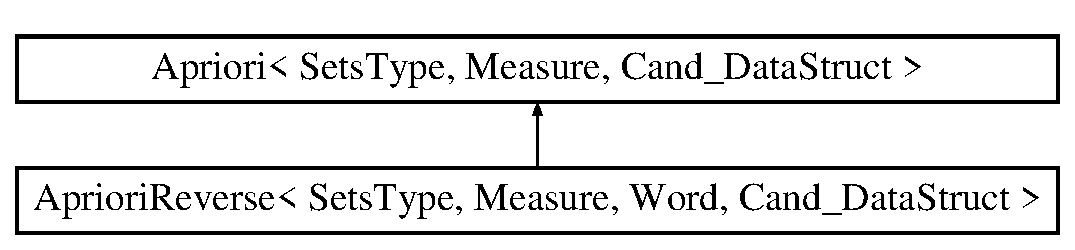
\includegraphics[height=2cm]{class_apriori_reverse}
\end{center}
\end{figure}
\subsection*{Public Member Functions}
\begin{CompactItemize}
\item 
{\bf Apriori\-Reverse} ()\label{class_apriori_reverse_18dd0f31ac2d8bc6d9036be8104bb6b8}

\begin{CompactList}\small\item\em Constructor. \item\end{CompactList}\item 
template$<$class Init\-Functor, class Predicate, class Output\-Theory, class Output\-Bd\-P, class Output\-Bd\-N, class f$>$ void {\bf operator()} (Init\-Functor \&init, {\bf Predicate} \&pred, Output\-Theory $\ast$theory, Output\-Bd\-P $\ast$bd\-P, Output\-Bd\-N $\ast$bd\-N, f \&word\-To\-Set)
\begin{CompactList}\small\item\em Functor operator that executes the algorithm. \item\end{CompactList}\item 
template$<$class Init\-Functor, class Predicate, class Output\-Theory, class Output\-Bd\-P, class Output\-Bd\-N$>$ void {\bf operator()} (Init\-Functor \&init, {\bf Predicate} \&pred, Output\-Theory $\ast$theory, Output\-Bd\-P $\ast$bd\-P, Output\-Bd\-N $\ast$bd\-N)
\begin{CompactList}\small\item\em Functor operator that executes the algorithm. \item\end{CompactList}\item 
template$<$class Init\-Functor, class Predicate, class Output\-Theory, class Output\-Bd\-P, class Output\-Bd\-N, class f, class Stop\-Iteration$>$ void {\bf operator()} (Init\-Functor \&init, {\bf Predicate} \&pred, Output\-Theory $\ast$theory, Output\-Bd\-P $\ast$bd\-P, Output\-Bd\-N $\ast$bd\-N, Stop\-Iteration $\ast$stop\-Ite, f \&word\-To\-Set)
\begin{CompactList}\small\item\em Functor operator that executes the algorithm and stop his execution when the functor passed in parameter return false. \item\end{CompactList}\item 
template$<$class Init\-Functor, class Predicate, class Output\-Theory, class Output\-Bd\-P, class Output\-Bd\-N, class Stop\-Iteration$>$ void {\bf operator()} (Init\-Functor \&init, {\bf Predicate} \&pred, Output\-Theory $\ast$theory, Output\-Bd\-P $\ast$bd\-P, Output\-Bd\-N $\ast$bd\-N, Stop\-Iteration $\ast$stop\-Ite)
\begin{CompactList}\small\item\em Functor operator that executes the algorithm and stop his execution when the functor passed in parameter return false. \item\end{CompactList}\end{CompactItemize}


\subsection{Detailed Description}
\subsubsection*{template$<$class Sets\-Type = int, class Measure = Boolean, class Word = vector$<$ Sets\-Type $>$, class Cand\_\-Data\-Struct = PTree$<$Sets\-Type,Measure$>$$>$ class Apriori\-Reverse$<$ Sets\-Type, Measure, Word, Cand\_\-Data\-Struct $>$}

Functor finding the theory and/or the negative border and/or the positive border using the {\bf Apriori}{\rm (p.\,\pageref{class_apriori})} strategy but with a top down exploration of the search space. 

Moreover this class enables to stop the execution of the algorithm at an iteration wrt to a user defined functor. The template parameter Sets\-Type represents the type of the sets representing the elements of the language. The template parameter Measure is the type of the value eventually associated with the word of the language. The template parameter Cand\_\-Data\-Struct is the data structure type used to store the candidates generated by the algorithms. The template parameter Word represents the type of the elements of the language. 



\subsection{Member Function Documentation}
\index{AprioriReverse@{Apriori\-Reverse}!operator()@{operator()}}
\index{operator()@{operator()}!AprioriReverse@{Apriori\-Reverse}}
\subsubsection{\setlength{\rightskip}{0pt plus 5cm}template$<$class Sets\-Type = int, class Measure = Boolean, class Word = vector$<$ Sets\-Type $>$, class Cand\_\-Data\-Struct = PTree$<$Sets\-Type,Measure$>$$>$ template$<$class Init\-Functor, class Predicate, class Output\-Theory, class Output\-Bd\-P, class Output\-Bd\-N, class Stop\-Iteration$>$ void {\bf Apriori\-Reverse}$<$ Sets\-Type, Measure, Word, Cand\_\-Data\-Struct $>$::operator() (Init\-Functor \& {\em init}, {\bf Predicate} \& {\em pred}, Output\-Theory $\ast$ {\em theory}, Output\-Bd\-P $\ast$ {\em bd\-P}, Output\-Bd\-N $\ast$ {\em bd\-N}, Stop\-Iteration $\ast$ {\em stop\-Ite})\hspace{0.3cm}{\tt  [inline]}}\label{class_apriori_reverse_a8018f226acaaa0047cf1386ed189e08}


Functor operator that executes the algorithm and stop his execution when the functor passed in parameter return false. 

\begin{Desc}
\item[Parameters:]
\begin{description}
\item[{\em init}]functor initializing the interesting items wrt predicate. \item[{\em pred}]the predicate \item[{\em theory}]output the theory in the given objet (must have a push\_\-back( container, measure ) method). \item[{\em bd\-P}]output the positive border in the given objet (must have a push\_\-back( container, measure ) method). \item[{\em bd\-N}]output the negative border in the given objet (must have a push\_\-back( container, measure ) method). \item[{\em stop\-Ite}]functor stop that stop the execution of the algorithm before the end. \item[{\em word\-To\-Set}]transform words of the language studied in sets. \end{description}
\end{Desc}


Reimplemented from {\bf Apriori$<$ Sets\-Type, Measure, Cand\_\-Data\-Struct $>$} {\rm (p.\,\pageref{class_apriori_117edc08779546395973171927fb8a77})}.\index{AprioriReverse@{Apriori\-Reverse}!operator()@{operator()}}
\index{operator()@{operator()}!AprioriReverse@{Apriori\-Reverse}}
\subsubsection{\setlength{\rightskip}{0pt plus 5cm}template$<$class Sets\-Type = int, class Measure = Boolean, class Word = vector$<$ Sets\-Type $>$, class Cand\_\-Data\-Struct = PTree$<$Sets\-Type,Measure$>$$>$ template$<$class Init\-Functor, class Predicate, class Output\-Theory, class Output\-Bd\-P, class Output\-Bd\-N, class f, class Stop\-Iteration$>$ void {\bf Apriori\-Reverse}$<$ Sets\-Type, Measure, Word, Cand\_\-Data\-Struct $>$::operator() (Init\-Functor \& {\em init}, {\bf Predicate} \& {\em pred}, Output\-Theory $\ast$ {\em theory}, Output\-Bd\-P $\ast$ {\em bd\-P}, Output\-Bd\-N $\ast$ {\em bd\-N}, Stop\-Iteration $\ast$ {\em stop\-Ite}, f \& {\em word\-To\-Set})\hspace{0.3cm}{\tt  [inline]}}\label{class_apriori_reverse_d898f211e89442230c64651031388e3d}


Functor operator that executes the algorithm and stop his execution when the functor passed in parameter return false. 

\begin{Desc}
\item[Parameters:]
\begin{description}
\item[{\em init}]functor initializing the interesting items wrt predicate. \item[{\em pred}]the predicate \item[{\em theory}]output the theory in the given objet (must have a push\_\-back( container, measure ) method). \item[{\em bd\-P}]output the positive border in the given objet (must have a push\_\-back( container, measure ) method). \item[{\em bd\-N}]output the negative border in the given objet (must have a push\_\-back( container, measure ) method). \item[{\em stop\-Ite}]functor stop that stop the execution of the algorithm before the end. \item[{\em word\-To\-Set}]transform words of the language studied in sets. \end{description}
\end{Desc}


Reimplemented from {\bf Apriori$<$ Sets\-Type, Measure, Cand\_\-Data\-Struct $>$} {\rm (p.\,\pageref{class_apriori_4ccc3fe5ae7ecaa9efffcdc41d1888ed})}.\index{AprioriReverse@{Apriori\-Reverse}!operator()@{operator()}}
\index{operator()@{operator()}!AprioriReverse@{Apriori\-Reverse}}
\subsubsection{\setlength{\rightskip}{0pt plus 5cm}template$<$class Sets\-Type = int, class Measure = Boolean, class Word = vector$<$ Sets\-Type $>$, class Cand\_\-Data\-Struct = PTree$<$Sets\-Type,Measure$>$$>$ template$<$class Init\-Functor, class Predicate, class Output\-Theory, class Output\-Bd\-P, class Output\-Bd\-N$>$ void {\bf Apriori\-Reverse}$<$ Sets\-Type, Measure, Word, Cand\_\-Data\-Struct $>$::operator() (Init\-Functor \& {\em init}, {\bf Predicate} \& {\em pred}, Output\-Theory $\ast$ {\em theory}, Output\-Bd\-P $\ast$ {\em bd\-P}, Output\-Bd\-N $\ast$ {\em bd\-N})\hspace{0.3cm}{\tt  [inline]}}\label{class_apriori_reverse_5266cde8d5a9455c9f9281e435754ca9}


Functor operator that executes the algorithm. 

\begin{Desc}
\item[Parameters:]
\begin{description}
\item[{\em init}]functor initializing the interesting items wrt predicate. \item[{\em pred}]the predicate \item[{\em theory}]output the theory in the given objet (must have a push\_\-back( container, measure ) method). \item[{\em bd\-P}]output the positive border in the given objet (must have a push\_\-back( container, measure ) method). \item[{\em bd\-N}]output the negative border in the given objet (must have a push\_\-back( container, measure ) method). \end{description}
\end{Desc}


Reimplemented from {\bf Apriori$<$ Sets\-Type, Measure, Cand\_\-Data\-Struct $>$} {\rm (p.\,\pageref{class_apriori_f0a2087314d1753cc3dd397c4a3f3dda})}.\index{AprioriReverse@{Apriori\-Reverse}!operator()@{operator()}}
\index{operator()@{operator()}!AprioriReverse@{Apriori\-Reverse}}
\subsubsection{\setlength{\rightskip}{0pt plus 5cm}template$<$class Sets\-Type = int, class Measure = Boolean, class Word = vector$<$ Sets\-Type $>$, class Cand\_\-Data\-Struct = PTree$<$Sets\-Type,Measure$>$$>$ template$<$class Init\-Functor, class Predicate, class Output\-Theory, class Output\-Bd\-P, class Output\-Bd\-N, class f$>$ void {\bf Apriori\-Reverse}$<$ Sets\-Type, Measure, Word, Cand\_\-Data\-Struct $>$::operator() (Init\-Functor \& {\em init}, {\bf Predicate} \& {\em pred}, Output\-Theory $\ast$ {\em theory}, Output\-Bd\-P $\ast$ {\em bd\-P}, Output\-Bd\-N $\ast$ {\em bd\-N}, f \& {\em word\-To\-Set})\hspace{0.3cm}{\tt  [inline]}}\label{class_apriori_reverse_f82618122967f0c6da9c4de5ea60a367}


Functor operator that executes the algorithm. 

\begin{Desc}
\item[Parameters:]
\begin{description}
\item[{\em init}]functor initializing the interesting items wrt predicate. \item[{\em pred}]the predicate \item[{\em theory}]output the theory in the given objet (must have a push\_\-back( container, measure ) method). \item[{\em bd\-P}]output the positive border in the given objet (must have a push\_\-back( container, measure ) method). \item[{\em bd\-N}]output the negative border in the given objet (must have a push\_\-back( container, measure ) method). \item[{\em word\-To\-Set}]transform words of the language studied in sets. \end{description}
\end{Desc}


Reimplemented from {\bf Apriori$<$ Sets\-Type, Measure, Cand\_\-Data\-Struct $>$} {\rm (p.\,\pageref{class_apriori_36d7a2cdad2a8c459f2b44e3ab460591})}.

The documentation for this class was generated from the following file:\begin{CompactItemize}
\item 
F:/i\-Zi/algorithms/Apriori\-Reverse.hxx\end{CompactItemize}

\section{Binary\-DB$<$ Sets\-Type, Data\-Struct\-DB $>$ Class Template Reference}
\label{class_binary_d_b}\index{BinaryDB@{BinaryDB}}
Binary\-DB\_\-base represents a binary relation, a transactionnal data bases.  


{\tt \#include $<$Binary\-DB.hxx$>$}

\subsection*{Public Types}
\begin{CompactItemize}
\item 
typedef {\bf It\-Binary\-DB}$<$ Sets\-Type, Data\-Struct\-DB $>$ {\bf iterator}\label{class_binary_d_b_48c97a6dac76e31fdc0ed035c2bfb29a}

\begin{CompactList}\small\item\em Used to have the same syntax that the STL. \item\end{CompactList}\end{CompactItemize}
\subsection*{Public Member Functions}
\begin{CompactItemize}
\item 
template$<$class Input\-Format$>$ {\bf Binary\-DB} (Input\-Format \&format, bool inverbose=false)
\begin{CompactList}\small\item\em Constructor. \item\end{CompactList}\item 
{\bf $\sim$Binary\-DB} ()\label{class_binary_d_b_f78c593365831c59be0862c601426dc9}

\begin{CompactList}\small\item\em Destructor. \item\end{CompactList}\item 
template$<$class Container$>$ void {\bf push\_\-back} (Container \&set\-Element, int nb=1)
\begin{CompactList}\small\item\em Push back a set of element. \item\end{CompactList}\item 
template$<$class Input\-Iterator$>$ void {\bf push\_\-back} (Input\-Iterator \&first, Input\-Iterator \&last, int nb=1)
\begin{CompactList}\small\item\em Push back a set of element. \item\end{CompactList}\item 
void {\bf set\-Recode} ({\bf Recode\-To\-Int}$<$ Sets\-Type $>$ $\ast$inrecode)\label{class_binary_d_b_374b531dec89c19bb50a2c3524c99da3}

\begin{CompactList}\small\item\em Set the recode function in the reconstructed data. \item\end{CompactList}\item 
{\bf It\-Binary\-DB}$<$ Sets\-Type, Data\-Struct\-DB $>$ {\bf begin} ()\label{class_binary_d_b_5add3a5a8f77c97c19be8a335c62783d}

\begin{CompactList}\small\item\em Return an iterator on the first element stored. \item\end{CompactList}\item 
{\bf It\-Binary\-DB}$<$ Sets\-Type, Data\-Struct\-DB $>$ {\bf end} ()\label{class_binary_d_b_33e5304e62ebff3fbf72f6088b800a97}

\begin{CompactList}\small\item\em Return an iterator on the element after the last element stored. \item\end{CompactList}\item 
Data\-Struct\-DB \& {\bf data} ()\label{class_binary_d_b_5fe8c3783aaae5426cddb38e15de7f69}

\begin{CompactList}\small\item\em Return the data. \item\end{CompactList}\end{CompactItemize}
\subsection*{Protected Attributes}
\begin{CompactItemize}
\item 
vector$<$ vector$<$ Sets\-Type $>$ $>$ $\ast$ {\bf tmp\-DB}\label{class_binary_d_b_9790b745395cb61d823ff9d9f7a2fede}

\begin{CompactList}\small\item\em Container used to store temporarly the transactions. \item\end{CompactList}\item 
Data\-Struct\-DB {\bf db}\label{class_binary_d_b_537da5448f8c18fd4eb840db2a11c05e}

\begin{CompactList}\small\item\em This container store the transactionnal database with ordered transactions of frequent items. \item\end{CompactList}\end{CompactItemize}
\subsection*{Friends}
\begin{CompactItemize}
\item 
class {\bf It\-Binary\-DB$<$ Sets\-Type, Data\-Struct\-DB $>$}\label{class_binary_d_b_2e8afe47ac8168f1f40b08eca702ffbf}

\end{CompactItemize}


\subsection{Detailed Description}
\subsubsection*{template$<$class Sets\-Type, class Data\-Struct\-DB = Tatree\_\-base$<$Sets\-Type$>$$>$ class Binary\-DB$<$ Sets\-Type, Data\-Struct\-DB $>$}

Binary\-DB\_\-base represents a binary relation, a transactionnal data bases. 

This class is used to store in memory the transactional database for frequent itemsets mining. By default, the transactions are stored in a trie data structure ({\bf Tatree}{\rm (p.\,\pageref{class_tatree})}). First, the transactions are stored in a temporary data structure (matrix). From this structure, the frequent items are extracted and reordered. After this, the transactions are recontructed (without not frequent items and in increasing oreder of support) and inserted in the final data structure.

The template parameter Sets\-Type is the type of the elements stored in the db. The template parameter Data\-Struct\-DB is a container of sets to store the transactions in memory. 



\subsection{Constructor \& Destructor Documentation}
\index{BinaryDB@{Binary\-DB}!BinaryDB@{BinaryDB}}
\index{BinaryDB@{BinaryDB}!BinaryDB@{Binary\-DB}}
\subsubsection{\setlength{\rightskip}{0pt plus 5cm}template$<$class Sets\-Type, class Data\-Struct\-DB = Tatree\_\-base$<$Sets\-Type$>$$>$ template$<$class Input\-Format$>$ {\bf Binary\-DB}$<$ Sets\-Type, Data\-Struct\-DB $>$::{\bf Binary\-DB} (Input\-Format \& {\em format}, bool {\em inverbose} = {\tt false})\hspace{0.3cm}{\tt  [inline]}}\label{class_binary_d_b_c5adea668e389622e005e7b5d0d50236}


Constructor. 

The constructor transfer the data from the input stream to a temporay data structure. The template parameter is a stream manipulator that input the data from the db. 

\subsection{Member Function Documentation}
\index{BinaryDB@{Binary\-DB}!push_back@{push\_\-back}}
\index{push_back@{push\_\-back}!BinaryDB@{Binary\-DB}}
\subsubsection{\setlength{\rightskip}{0pt plus 5cm}template$<$class Sets\-Type, class Data\-Struct\-DB = Tatree\_\-base$<$Sets\-Type$>$$>$ template$<$class Input\-Iterator$>$ void {\bf Binary\-DB}$<$ Sets\-Type, Data\-Struct\-DB $>$::push\_\-back (Input\-Iterator \& {\em first}, Input\-Iterator \& {\em last}, int {\em nb} = {\tt 1})\hspace{0.3cm}{\tt  [inline]}}\label{class_binary_d_b_d91fcffa6875b442c3994a2ea51d471a}


Push back a set of element. 

This function insert a transaction in the final data structure. With default parameter, the template parameter represents the input iterators on the elements to insert in the data base. \begin{Desc}
\item[Parameters:]
\begin{description}
\item[{\em first}]iterator on the first element \item[{\em last}]iterator on the element after the last \item[{\em nb}]the number of times the set is inserted \end{description}
\end{Desc}
\index{BinaryDB@{Binary\-DB}!push_back@{push\_\-back}}
\index{push_back@{push\_\-back}!BinaryDB@{Binary\-DB}}
\subsubsection{\setlength{\rightskip}{0pt plus 5cm}template$<$class Sets\-Type, class Data\-Struct\-DB = Tatree\_\-base$<$Sets\-Type$>$$>$ template$<$class Container$>$ void {\bf Binary\-DB}$<$ Sets\-Type, Data\-Struct\-DB $>$::push\_\-back (Container \& {\em set\-Element}, int {\em nb} = {\tt 1})\hspace{0.3cm}{\tt  [inline]}}\label{class_binary_d_b_14ff7dc20fded0c3fddc065318fc2b58}


Push back a set of element. 

This function insert a transaction in the final data structure. With default parameter, this function corresponds to the classic {\bf push\_\-back( )}{\rm (p.\,\pageref{class_binary_d_b_14ff7dc20fded0c3fddc065318fc2b58})} function od STL container. The template parameter represents a container of element of type Sets\-Type. \begin{Desc}
\item[Parameters:]
\begin{description}
\item[{\em set\-Element}]the set of element to insert in the trie \item[{\em nb}]the number of times the set is inserted \end{description}
\end{Desc}


The documentation for this class was generated from the following file:\begin{CompactItemize}
\item 
F:/i\-Zi/data/memory/Binary\-DB.hxx\end{CompactItemize}

\section{Boolean Class Reference}
\label{class_boolean}\index{Boolean@{Boolean}}
{\bf Boolean}{\rm (p.\,\pageref{class_boolean})} type.  


{\tt \#include $<$Boolean.hpp$>$}



\subsection{Detailed Description}
{\bf Boolean}{\rm (p.\,\pageref{class_boolean})} type. 

This class is created since their is a problem with vector$<$bool$>$::iterator in the STL. It returns a temporary \_\-Bit\_\-Reference rather than a \char`\"{}proper\char`\"{} reference. Vector$<$bool$>$ isn't a proper container and it's iterators don't satisfy the conditions for forward iterators. For more details see: {\tt http://gcc.gnu.org/ml/libstdc++/2005-03/msg00148.html} 



The documentation for this class was generated from the following file:\begin{CompactItemize}
\item 
F:/i\-Zi/util/Boolean.hpp\end{CompactItemize}

\section{Complement$<$ Sets\-Type $>$ Class Template Reference}
\label{class_complement}\index{Complement@{Complement}}
Functor that complements a set.  


{\tt \#include $<$Complement.hxx$>$}

\subsection*{Public Member Functions}
\begin{CompactItemize}
\item 
{\bf Complement} ()\label{class_complement_355fbb3afb3439453e2f5cbec085fd6f}

\begin{CompactList}\small\item\em constructor \item\end{CompactList}\item 
template$<$class Iterator\-Set$>$ vector$<$ Sets\-Type $>$ $\ast$ {\bf operator()} (Iterator\-Set s)
\begin{CompactList}\small\item\em Operator returning the complement of a set. \item\end{CompactList}\item 
template$<$class Iterator\-Set$>$ vector$<$ Sets\-Type $>$ $\ast$ {\bf inverse} (Iterator\-Set s)
\begin{CompactList}\small\item\em Method returning the complement of a set. \item\end{CompactList}\end{CompactItemize}
\subsection*{Public Attributes}
\begin{CompactItemize}
\item 
vector$<$ Sets\-Type $>$ $\ast$ {\bf list\-Elements}
\begin{CompactList}\small\item\em list of elements of size 1 \item\end{CompactList}\end{CompactItemize}


\subsection{Detailed Description}
\subsubsection*{template$<$class Sets\-Type$>$ class Complement$<$ Sets\-Type $>$}

Functor that complements a set. 

The template parameter Sets\-Type is the type of the elements. 



\subsection{Member Function Documentation}
\index{Complement@{Complement}!inverse@{inverse}}
\index{inverse@{inverse}!Complement@{Complement}}
\subsubsection{\setlength{\rightskip}{0pt plus 5cm}template$<$class Sets\-Type$>$ template$<$class Iterator\-Set$>$ vector$<$Sets\-Type$>$$\ast$ {\bf Complement}$<$ Sets\-Type $>$::inverse (Iterator\-Set {\em s})\hspace{0.3cm}{\tt  [inline]}}\label{class_complement_9ff19c9282b649fa59746307d5cbdac7}


Method returning the complement of a set. 

\begin{Desc}
\item[Parameters:]
\begin{description}
\item[{\em s}]set to complement \end{description}
\end{Desc}
\index{Complement@{Complement}!operator()@{operator()}}
\index{operator()@{operator()}!Complement@{Complement}}
\subsubsection{\setlength{\rightskip}{0pt plus 5cm}template$<$class Sets\-Type$>$ template$<$class Iterator\-Set$>$ vector$<$Sets\-Type$>$$\ast$ {\bf Complement}$<$ Sets\-Type $>$::operator() (Iterator\-Set {\em s})\hspace{0.3cm}{\tt  [inline]}}\label{class_complement_8d910fa02f315d52a24b0ec094fc54f7}


Operator returning the complement of a set. 

\begin{Desc}
\item[Parameters:]
\begin{description}
\item[{\em s}]set to complement \end{description}
\end{Desc}


\subsection{Member Data Documentation}
\index{Complement@{Complement}!listElements@{listElements}}
\index{listElements@{listElements}!Complement@{Complement}}
\subsubsection{\setlength{\rightskip}{0pt plus 5cm}template$<$class Sets\-Type$>$ vector$<$Sets\-Type$>$$\ast$ {\bf Complement}$<$ Sets\-Type $>$::{\bf list\-Elements}}\label{class_complement_85fe06434f6f05ec14db39233f35e26f}


list of elements of size 1 

It musts be initialized before using the functor. 

The documentation for this class was generated from the following file:\begin{CompactItemize}
\item 
F:/i\-Zi/algorithms/Complement.hxx\end{CompactItemize}

\section{Essential$<$ Data, Sets\-Type $>$ Class Template Reference}
\label{class_essential}\index{Essential@{Essential}}
Functor representing the predicate being frequent essential.  


{\tt \#include $<$Essential.hxx$>$}

Inheritance diagram for Essential$<$ Data, Sets\-Type $>$::\begin{figure}[H]
\begin{center}
\leavevmode
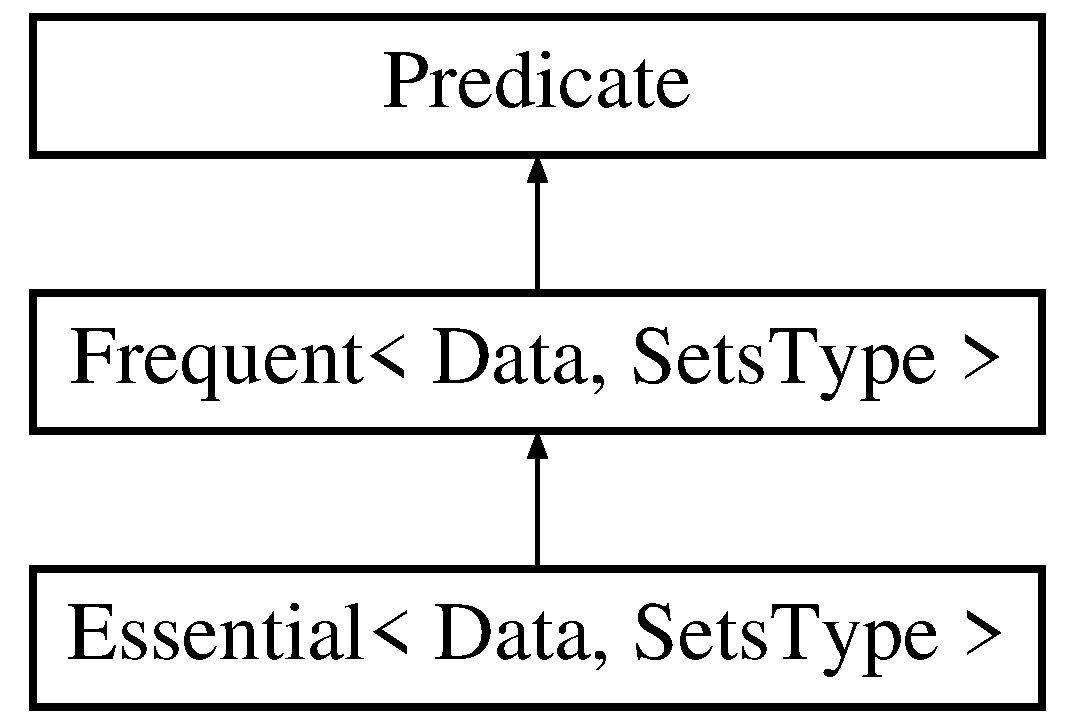
\includegraphics[height=3cm]{class_essential}
\end{center}
\end{figure}
\subsection*{Public Member Functions}
\begin{CompactItemize}
\item 
{\bf Essential} (Data \&indb, int in\-Minsup)
\begin{CompactList}\small\item\em Constructor. \item\end{CompactList}\item 
{\bf $\sim$Essential} ()\label{class_essential_a4f54ab8615df753dffc0a4d64af6c63}

\begin{CompactList}\small\item\em Destructor. \item\end{CompactList}\item 
template$<$class Iterator, class Measure$>$ bool {\bf operator()} (Iterator itemset\-It, Measure \&mes\-Cand)
\begin{CompactList}\small\item\em Operator that test if an itemet is frequent or not. \item\end{CompactList}\end{CompactItemize}


\subsection{Detailed Description}
\subsubsection*{template$<$class Data, class Sets\-Type$>$ class Essential$<$ Data, Sets\-Type $>$}

Functor representing the predicate being frequent essential. 

This functor test if an itemset is frequent and essential. This functor process the support and the disjunction before pruning. We suppose that the data has the same internal encoding than the candidates (ie, the first item met is recoded in \char`\"{}0\char`\"{}, the second in \char`\"{}1\char`\"{}, ...).

The methods of this predicate are specific to tries data structure ({\bf PTree}{\rm (p.\,\pageref{class_p_tree})} for the candiates and {\bf Tatree}{\rm (p.\,\pageref{class_tatree})} for the transactions). For the moment, this functor can only be used when using a levelwise exploration of the search space ({\bf Apriori}{\rm (p.\,\pageref{class_apriori})}) since it checks for subsets already generated.

The template parameter Data is the type of the transactional database. The template parameter Sets\-Type is the type of the items. 



\subsection{Constructor \& Destructor Documentation}
\index{Essential@{Essential}!Essential@{Essential}}
\index{Essential@{Essential}!Essential@{Essential}}
\subsubsection{\setlength{\rightskip}{0pt plus 5cm}template$<$class Data, class Sets\-Type$>$ {\bf Essential}$<$ Data, Sets\-Type $>$::{\bf Essential} (Data \& {\em indb}, int {\em in\-Minsup})\hspace{0.3cm}{\tt  [inline]}}\label{class_essential_c47b2c4a5a736b4f0d6d6da070d3f3ed}


Constructor. 

\begin{Desc}
\item[Parameters:]
\begin{description}
\item[{\em indb}]the transactional database \item[{\em in\-Minsup}]the absolute minimum support threshold \end{description}
\end{Desc}


\subsection{Member Function Documentation}
\index{Essential@{Essential}!operator()@{operator()}}
\index{operator()@{operator()}!Essential@{Essential}}
\subsubsection{\setlength{\rightskip}{0pt plus 5cm}template$<$class Data, class Sets\-Type$>$ template$<$class Iterator, class Measure$>$ bool {\bf Essential}$<$ Data, Sets\-Type $>$::operator() (Iterator {\em itemset\-It}, Measure \& {\em mes\-Cand})\hspace{0.3cm}{\tt  [inline]}}\label{class_essential_e6a89fa2543fe441619066b0f4f6323b}


Operator that test if an itemet is frequent or not. 

\begin{Desc}
\item[Parameters:]
\begin{description}
\item[{\em itemset\-It}]iterator (or pointer) on the itemset to test wrt the predicate \item[{\em mes\-Cand}]value of the support of the itemset \end{description}
\end{Desc}


Reimplemented from {\bf Frequent$<$ Data, Sets\-Type $>$} {\rm (p.\,\pageref{class_frequent_82e02ab1cf1749ea52e9603dc06a5d15})}.

The documentation for this class was generated from the following file:\begin{CompactItemize}
\item 
F:/i\-Zi/problems/essential/Essential.hxx\end{CompactItemize}

\section{Fdep\-File Class Reference}
\label{class_fdep_file}\index{FdepFile@{FdepFile}}
Read a relation saved in the Fdep format.  


{\tt \#include $<$Fdep\-File.hxx$>$}

\subsection*{Public Member Functions}
\begin{CompactItemize}
\item 
{\bf Fdep\-File} (char $\ast$in\-File\-Name)\label{class_fdep_file_56ef78c6ca2658e52a2e07d985d41b23}

\begin{CompactList}\small\item\em Constructor. \item\end{CompactList}\item 
virtual {\bf $\sim$Fdep\-File} ()
\begin{CompactList}\small\item\em Destructor. \item\end{CompactList}\item 
template$<$class Container\-DB$>$ {\bf Fdep\-File} \& {\bf operator$>$$>$} (Container\-DB \&container)
\begin{CompactList}\small\item\em Extract data of the file and insert it in a container. \item\end{CompactList}\end{CompactItemize}
\subsection*{Public Attributes}
\begin{CompactItemize}
\item 
vector$<$ string $>$ {\bf attributes}\label{class_fdep_file_2a716ed1ecb7dfc8897266aa00a8ce69}

\begin{CompactList}\small\item\em List of all the attributes. \item\end{CompactList}\end{CompactItemize}
\subsection*{Protected Attributes}
\begin{CompactItemize}
\item 
char $\ast$ {\bf file\-Name}\label{class_fdep_file_782e7766a7e9d68e8e84fafb61091817}

\begin{CompactList}\small\item\em name of the file to used \item\end{CompactList}\item 
ifstream {\bf readfile}\label{class_fdep_file_304ecc5605a362550142890ad870e75d}

\begin{CompactList}\small\item\em Stream used to read in the file. \item\end{CompactList}\item 
ofstream {\bf writefile}\label{class_fdep_file_47977170ade83f313f6755a0ead51056}

\begin{CompactList}\small\item\em Stream used to write in the file. \item\end{CompactList}\end{CompactItemize}


\subsection{Detailed Description}
Read a relation saved in the Fdep format. 

The file format is: first line: the relation schema relation( rel-head, [ attr-1, attr-2, ..., attr-n ]), with rel-head the name of the relation, attr-i th name of the ith attribute. each other line: one tuple rel-head( value-of-attr-1, ..., value-of-attr-n ).

see for more details: {\tt http://www.cs.bris.ac.uk/$\sim$flach/fdep/} 



\subsection{Constructor \& Destructor Documentation}
\index{FdepFile@{Fdep\-File}!~FdepFile@{$\sim$FdepFile}}
\index{~FdepFile@{$\sim$FdepFile}!FdepFile@{Fdep\-File}}
\subsubsection{\setlength{\rightskip}{0pt plus 5cm}virtual Fdep\-File::$\sim$Fdep\-File ()\hspace{0.3cm}{\tt  [inline, virtual]}}\label{class_fdep_file_7f24ec32454849c0756eab48780f02db}


Destructor. 

The destructor close the file. 

\subsection{Member Function Documentation}
\index{FdepFile@{Fdep\-File}!operator>>@{operator$>$$>$}}
\index{operator>>@{operator$>$$>$}!FdepFile@{Fdep\-File}}
\subsubsection{\setlength{\rightskip}{0pt plus 5cm}template$<$class Container\-DB$>$ {\bf Fdep\-File}\& Fdep\-File::operator$>$$>$ (Container\-DB \& {\em container})\hspace{0.3cm}{\tt  [inline]}}\label{class_fdep_file_bc7b742550cb389f78468e52cf4d9b59}


Extract data of the file and insert it in a container. 

\begin{Desc}
\item[Parameters:]
\begin{description}
\item[{\em container}]where the data read is inserted (must have a push\_\-back function). \end{description}
\end{Desc}
\begin{Desc}
\item[Returns:]$\ast$this. \end{Desc}


The documentation for this class was generated from the following file:\begin{CompactItemize}
\item 
F:/i\-Zi/data/file/Fdep\-File.hxx\end{CompactItemize}

\section{Fimi\-File$<$ Sets\-Type $>$ Class Template Reference}
\label{class_fimi_file}\index{FimiFile@{FimiFile}}
Class used to read a transactionnal db in the FIMI format and save data in the FIMI format.  


{\tt \#include $<$Fimi\-File.hxx$>$}

\subsection*{Public Types}
\begin{CompactItemize}
\item 
typedef {\bf It\-Fimi\-File}$<$ Sets\-Type $>$ {\bf iterator}\label{class_fimi_file_31e6c824ac439296b7aa5701d07d81f5}

\begin{CompactList}\small\item\em Used to have the same syntax tha the STL. \item\end{CompactList}\end{CompactItemize}
\subsection*{Public Member Functions}
\begin{CompactItemize}
\item 
{\bf Fimi\-File} (const char $\ast$in\-File\-Name)\label{class_fimi_file_0698069b454374417db777ad6f4cfcfb}

\begin{CompactList}\small\item\em Constructor. \item\end{CompactList}\item 
virtual {\bf $\sim$Fimi\-File} ()
\begin{CompactList}\small\item\em Destructor. \item\end{CompactList}\item 
template$<$class Container\-DB$>$ {\bf Fimi\-File} \& {\bf operator$>$$>$} (Container\-DB \&container)
\begin{CompactList}\small\item\em Extract data of the file and insert it in a container. \item\end{CompactList}\item 
template$<$class Container\-Bd\-T$>$ {\bf Fimi\-File} \& {\bf operator$<$$<$} (Container\-Bd\-T \&container)
\begin{CompactList}\small\item\em Extract all the data of the container and insert it in a file . \item\end{CompactList}\item 
template$<$class Container, class Val$>$ void {\bf push\_\-back} (Container \&set\-Element, Val supp)
\begin{CompactList}\small\item\em Insert an itemset in the file. \item\end{CompactList}\item 
template$<$class Container$>$ void {\bf push\_\-back} (Container \&set\-Element)
\begin{CompactList}\small\item\em Insert an itemset in the file. \item\end{CompactList}\item 
template$<$class Input\-Iterator, class Val$>$ void {\bf push\_\-back} (Input\-Iterator first, Input\-Iterator last, Val supp)
\begin{CompactList}\small\item\em Insert a set of element in the file. \item\end{CompactList}\item 
{\bf It\-Fimi\-File}$<$ Sets\-Type $>$ {\bf begin} ()\label{class_fimi_file_805ab6183fa800eddda7f8f1a72094e0}

\begin{CompactList}\small\item\em Return an iterator on the first element stored. \item\end{CompactList}\item 
{\bf It\-Fimi\-File}$<$ Sets\-Type $>$ {\bf end} ()\label{class_fimi_file_40d4c8c8d693bdb4b93ba601928e15d7}

\begin{CompactList}\small\item\em Return an iterator on the element after the last element stored. \item\end{CompactList}\item 
void {\bf close} ()\label{class_fimi_file_d4bb3dfd03745838c7a232e001a1eb7a}

\begin{CompactList}\small\item\em Close the file. \item\end{CompactList}\end{CompactItemize}
\subsection*{Protected Member Functions}
\begin{CompactItemize}
\item 
bool {\bf read\-Line} (vector$<$ int $>$ \&line)
\begin{CompactList}\small\item\em Function reading a line of integer in the file. \item\end{CompactList}\item 
template$<$class Container$>$ bool {\bf read\-Line} (Container \&line)
\begin{CompactList}\small\item\em Function reading a line in the file. \item\end{CompactList}\item 
template$<$class Container\-DB$>$ bool {\bf read} (Container\-DB \&container)
\begin{CompactList}\small\item\em Function reading all the data in the file and store it in a container. \item\end{CompactList}\item 
template$<$class Iterator, class Val$>$ void {\bf write} (Iterator begin, Iterator end, Val measure)
\begin{CompactList}\small\item\em Function write data in a file. \item\end{CompactList}\end{CompactItemize}
\subsection*{Protected Attributes}
\begin{CompactItemize}
\item 
const char $\ast$ {\bf file\-Name}\label{class_fimi_file_798e7dd3a0fb30f74d14d371b380329d}

\begin{CompactList}\small\item\em name of the file to used \item\end{CompactList}\item 
ifstream {\bf readfile}\label{class_fimi_file_6e6ce86565764314471aaf478639fd2c}

\begin{CompactList}\small\item\em Stream used to read in the file. \item\end{CompactList}\item 
ofstream {\bf writefile}\label{class_fimi_file_c3caf86aea00e29476a21d1285fd7c77}

\begin{CompactList}\small\item\em Stream used to write in the file. \item\end{CompactList}\end{CompactItemize}
\subsection*{Friends}
\begin{CompactItemize}
\item 
class {\bf It\-Fimi\-File$<$ Sets\-Type $>$}\label{class_fimi_file_8a239185a8893ca8f127ab8909bb9ee7}

\end{CompactItemize}
\subsection*{Classes}
\begin{CompactItemize}
\item 
class {\bf save\-Container\-In\-File}
\begin{CompactList}\small\item\em Functor used to save in the file each set. \item\end{CompactList}\item 
class {\bf save\-Elem\-In\-File}
\begin{CompactList}\small\item\em Functor used to save in the file each element of a set. \item\end{CompactList}\end{CompactItemize}


\subsection{Detailed Description}
\subsubsection*{template$<$class Sets\-Type = int$>$ class Fimi\-File$<$ Sets\-Type $>$}

Class used to read a transactionnal db in the FIMI format and save data in the FIMI format. 

This class is implemented uidung the stream classes of the iostream library. Consequently, it is less efficient thant the correspondig C class. The template parameter Sets\-Type is the type of items in the transactions. 



\subsection{Constructor \& Destructor Documentation}
\index{FimiFile@{Fimi\-File}!~FimiFile@{$\sim$FimiFile}}
\index{~FimiFile@{$\sim$FimiFile}!FimiFile@{Fimi\-File}}
\subsubsection{\setlength{\rightskip}{0pt plus 5cm}template$<$class Sets\-Type = int$>$ virtual {\bf Fimi\-File}$<$ Sets\-Type $>$::$\sim${\bf Fimi\-File} ()\hspace{0.3cm}{\tt  [inline, virtual]}}\label{class_fimi_file_755603ee01f5dbb89246a62211bdd63f}


Destructor. 

The destructor close the file. 

\subsection{Member Function Documentation}
\index{FimiFile@{Fimi\-File}!operator<<@{operator$<$$<$}}
\index{operator<<@{operator$<$$<$}!FimiFile@{Fimi\-File}}
\subsubsection{\setlength{\rightskip}{0pt plus 5cm}template$<$class Sets\-Type = int$>$ template$<$class Container\-Bd\-T$>$ {\bf Fimi\-File}\& {\bf Fimi\-File}$<$ Sets\-Type $>$::operator$<$$<$ (Container\-Bd\-T \& {\em container})\hspace{0.3cm}{\tt  [inline]}}\label{class_fimi_file_79e4b235b956e9a1965176be3672a6ce}


Extract all the data of the container and insert it in a file . 

\begin{Desc}
\item[Parameters:]
\begin{description}
\item[{\em container}]where the data is read. \end{description}
\end{Desc}
\begin{Desc}
\item[Returns:]$\ast$this. \end{Desc}
\index{FimiFile@{Fimi\-File}!operator>>@{operator$>$$>$}}
\index{operator>>@{operator$>$$>$}!FimiFile@{Fimi\-File}}
\subsubsection{\setlength{\rightskip}{0pt plus 5cm}template$<$class Sets\-Type = int$>$ template$<$class Container\-DB$>$ {\bf Fimi\-File}\& {\bf Fimi\-File}$<$ Sets\-Type $>$::operator$>$$>$ (Container\-DB \& {\em container})\hspace{0.3cm}{\tt  [inline]}}\label{class_fimi_file_3d7feafbe9c9e71df3fda3e9514ebdef}


Extract data of the file and insert it in a container. 

\begin{Desc}
\item[Parameters:]
\begin{description}
\item[{\em container}]where the data read is inserted (must have a push\_\-back function). \end{description}
\end{Desc}
\begin{Desc}
\item[Returns:]$\ast$this. \end{Desc}
\index{FimiFile@{Fimi\-File}!push_back@{push\_\-back}}
\index{push_back@{push\_\-back}!FimiFile@{Fimi\-File}}
\subsubsection{\setlength{\rightskip}{0pt plus 5cm}template$<$class Sets\-Type = int$>$ template$<$class Input\-Iterator, class Val$>$ void {\bf Fimi\-File}$<$ Sets\-Type $>$::push\_\-back (Input\-Iterator {\em first}, Input\-Iterator {\em last}, Val {\em supp})\hspace{0.3cm}{\tt  [inline]}}\label{class_fimi_file_c01fb0d5fcf07c991fe85ca12ecd7a02}


Insert a set of element in the file. 

The template parameter represents the input iterators on the integers to insert in the file. \begin{Desc}
\item[Parameters:]
\begin{description}
\item[{\em first}]iterator on the first element. \item[{\em last}]iterator on the element after the last. \item[{\em supp}]the support of the itemset. \end{description}
\end{Desc}
\index{FimiFile@{Fimi\-File}!push_back@{push\_\-back}}
\index{push_back@{push\_\-back}!FimiFile@{Fimi\-File}}
\subsubsection{\setlength{\rightskip}{0pt plus 5cm}template$<$class Sets\-Type = int$>$ template$<$class Container$>$ void {\bf Fimi\-File}$<$ Sets\-Type $>$::push\_\-back (Container \& {\em set\-Element})\hspace{0.3cm}{\tt  [inline]}}\label{class_fimi_file_dae7226e9737797a445300151a5dd907}


Insert an itemset in the file. 

This function corresponds to the classic {\bf push\_\-back( )}{\rm (p.\,\pageref{class_fimi_file_72dce2f4bf0815c28fe52c951e51a1e0})} function od STL container. The template parameter represents a container of integers. \begin{Desc}
\item[Parameters:]
\begin{description}
\item[{\em set\-Element}]the set of element to insert in the file. \item[{\em supp}]the support of the itemset. \end{description}
\end{Desc}
\index{FimiFile@{Fimi\-File}!push_back@{push\_\-back}}
\index{push_back@{push\_\-back}!FimiFile@{Fimi\-File}}
\subsubsection{\setlength{\rightskip}{0pt plus 5cm}template$<$class Sets\-Type = int$>$ template$<$class Container, class Val$>$ void {\bf Fimi\-File}$<$ Sets\-Type $>$::push\_\-back (Container \& {\em set\-Element}, Val {\em supp})\hspace{0.3cm}{\tt  [inline]}}\label{class_fimi_file_72dce2f4bf0815c28fe52c951e51a1e0}


Insert an itemset in the file. 

This function corresponds to the classic {\bf push\_\-back( )}{\rm (p.\,\pageref{class_fimi_file_72dce2f4bf0815c28fe52c951e51a1e0})} function od STL container. The template parameter represents a container of integers. \begin{Desc}
\item[Parameters:]
\begin{description}
\item[{\em set\-Element}]the set of element to insert in the file. \item[{\em supp}]the support of the itemset. \end{description}
\end{Desc}
\index{FimiFile@{Fimi\-File}!read@{read}}
\index{read@{read}!FimiFile@{Fimi\-File}}
\subsubsection{\setlength{\rightskip}{0pt plus 5cm}template$<$class Sets\-Type$>$ template$<$class Container\-DB$>$ bool {\bf Fimi\-File}$<$ Sets\-Type $>$::read (Container\-DB \& {\em container})\hspace{0.3cm}{\tt  [protected]}}\label{class_fimi_file_841b304183b3c6d45b7cd1eae3c3497e}


Function reading all the data in the file and store it in a container. 

\begin{Desc}
\item[Parameters:]
\begin{description}
\item[{\em container}]class representing the relation (must have a push\_\-back function). \end{description}
\end{Desc}
\begin{Desc}
\item[Returns:]true if data has been read. \end{Desc}
\index{FimiFile@{Fimi\-File}!readLine@{readLine}}
\index{readLine@{readLine}!FimiFile@{Fimi\-File}}
\subsubsection{\setlength{\rightskip}{0pt plus 5cm}template$<$class Sets\-Type$>$ template$<$class Container$>$ bool {\bf Fimi\-File}$<$ Sets\-Type $>$::read\-Line (Container \& {\em line})\hspace{0.3cm}{\tt  [protected]}}\label{class_fimi_file_64466eb74b18b382f35c2ca4a939b0f9}


Function reading a line in the file. 

\begin{Desc}
\item[Parameters:]
\begin{description}
\item[{\em line}]stores the line (must have a push\_\-back function). \end{description}
\end{Desc}
\begin{Desc}
\item[Returns:]false if end of file \end{Desc}
\index{FimiFile@{Fimi\-File}!readLine@{readLine}}
\index{readLine@{readLine}!FimiFile@{Fimi\-File}}
\subsubsection{\setlength{\rightskip}{0pt plus 5cm}template$<$class Sets\-Type$>$ bool {\bf Fimi\-File}$<$ Sets\-Type $>$::read\-Line (vector$<$ int $>$ \& {\em line})\hspace{0.3cm}{\tt  [protected]}}\label{class_fimi_file_63c9a00918ab05006ef1dae5380f3e1d}


Function reading a line of integer in the file. 

\begin{Desc}
\item[Parameters:]
\begin{description}
\item[{\em line}]stores the line of integers in a vector. \end{description}
\end{Desc}
\begin{Desc}
\item[Returns:]false if end of file \end{Desc}
\index{FimiFile@{Fimi\-File}!write@{write}}
\index{write@{write}!FimiFile@{Fimi\-File}}
\subsubsection{\setlength{\rightskip}{0pt plus 5cm}template$<$class Sets\-Type = int$>$ template$<$class Iterator, class Val$>$ void {\bf Fimi\-File}$<$ Sets\-Type $>$::write (Iterator {\em begin}, Iterator {\em end}, Val {\em measure})\hspace{0.3cm}{\tt  [protected]}}\label{class_fimi_file_359f265cd495d244b21d7c3bbe271620}


Function write data in a file. 

\begin{Desc}
\item[Parameters:]
\begin{description}
\item[{\em begin}]iterator on the first element of the container to save \item[{\em supp}]the support of the itemset. \end{description}
\end{Desc}


The documentation for this class was generated from the following file:\begin{CompactItemize}
\item 
F:/i\-Zi/data/file/Fimi\-File.hxx\end{CompactItemize}

\section{Fimi\-File$<$ Sets\-Type $>$::save\-Container\-In\-File Class Reference}
\label{class_fimi_file_1_1save_container_in_file}\index{FimiFile::saveContainerInFile@{FimiFile::saveContainerInFile}}
Functor used to save in the file each set.  


{\tt \#include $<$Fimi\-File.hxx$>$}



\subsection{Detailed Description}
\subsubsection*{template$<$class Sets\-Type = int$>$ class Fimi\-File$<$ Sets\-Type $>$::save\-Container\-In\-File}

Functor used to save in the file each set. 



The documentation for this class was generated from the following file:\begin{CompactItemize}
\item 
F:/i\-Zi/data/file/Fimi\-File.hxx\end{CompactItemize}

\section{Fimi\-File$<$ Sets\-Type $>$::save\-Elem\-In\-File Class Reference}
\label{class_fimi_file_1_1save_elem_in_file}\index{FimiFile::saveElemInFile@{FimiFile::saveElemInFile}}
Functor used to save in the file each element of a set.  


{\tt \#include $<$Fimi\-File.hxx$>$}



\subsection{Detailed Description}
\subsubsection*{template$<$class Sets\-Type = int$>$ class Fimi\-File$<$ Sets\-Type $>$::save\-Elem\-In\-File}

Functor used to save in the file each element of a set. 



The documentation for this class was generated from the following file:\begin{CompactItemize}
\item 
F:/i\-Zi/data/file/Fimi\-File.hxx\end{CompactItemize}

\section{Fimi\-File\-C$<$ Container\-Trans $>$ Class Template Reference}
\label{class_fimi_file_c}\index{FimiFileC@{FimiFileC}}
Class used to read a transactionnal db in the FIMI format and save data in the FIMI format.  


{\tt \#include $<$Fimi\-File\-C.hxx$>$}

\subsection*{Public Types}
\begin{CompactItemize}
\item 
typedef {\bf It\-Fimi\-File}$<$ Container\-Trans $>$ {\bf iterator}\label{class_fimi_file_c_af735df6c6fcef8a0bd52f8c3fc46f28}

\begin{CompactList}\small\item\em Used to have the same syntax tha the STL. \item\end{CompactList}\end{CompactItemize}
\subsection*{Public Member Functions}
\begin{CompactItemize}
\item 
{\bf Fimi\-File\-C} (char $\ast$in\-File\-Name=0)
\begin{CompactList}\small\item\em Constructor. \item\end{CompactList}\item 
virtual {\bf $\sim$Fimi\-File\-C} ()
\begin{CompactList}\small\item\em Destructor. \item\end{CompactList}\item 
template$<$class Container\-Bd\-T$>$ {\bf Fimi\-File\-C} \& {\bf operator$>$$>$} (Container\-Bd\-T \&container)
\begin{CompactList}\small\item\em Extract all the data of the file and insert it in a container. \item\end{CompactList}\item 
template$<$class Container\-Bd\-T$>$ {\bf Fimi\-File\-C} \& {\bf operator$<$$<$} (Container\-Bd\-T \&container)
\begin{CompactList}\small\item\em Extract all the data of the container (set of itemsets) and insert it in the file. \item\end{CompactList}\item 
{\bf It\-Fimi\-File}$<$ Container\-Trans $>$ {\bf begin} ()\label{class_fimi_file_c_e89aafdad5202e8653be2892b2ea7dc5}

\begin{CompactList}\small\item\em Return an iterator on the first element stored. \item\end{CompactList}\item 
{\bf It\-Fimi\-File}$<$ Container\-Trans $>$ {\bf end} ()\label{class_fimi_file_c_c943eb9bd7e1a038ae002b4942d3fca8}

\begin{CompactList}\small\item\em Return an iterator on the element after the last element stored. \item\end{CompactList}\item 
template$<$class Container, class Val$>$ void {\bf push\_\-back} (Container \&set\-Element, Val supp)
\begin{CompactList}\small\item\em Insert an itemset in the file. \item\end{CompactList}\item 
template$<$class Input\-Iterator, class Val$>$ void {\bf push\_\-back} (Input\-Iterator first, Input\-Iterator last, Val supp)
\begin{CompactList}\small\item\em Insert a set of element in the file. \item\end{CompactList}\end{CompactItemize}
\subsection*{Protected Member Functions}
\begin{CompactItemize}
\item 
bool {\bf read\-Trans} (Container\-Trans \&trans)
\begin{CompactList}\small\item\em Function reading a transaction in the file. \item\end{CompactList}\item 
template$<$class Container\-Bd\-T$>$ bool {\bf read} (Container\-Bd\-T \&container)
\begin{CompactList}\small\item\em Function reading data in a file and store it in a container. \item\end{CompactList}\item 
template$<$class Iterator, class Val$>$ void {\bf write} (Iterator begin, Iterator end, Val supp)
\begin{CompactList}\small\item\em Function write data in a file. \item\end{CompactList}\item 
template$<$class Iterator$>$ void {\bf write} (Iterator begin, Iterator end, int supp)
\begin{CompactList}\small\item\em Function write data in a file when the value associated with the elements are integers. \item\end{CompactList}\end{CompactItemize}
\subsection*{Protected Attributes}
\begin{CompactItemize}
\item 
char $\ast$ {\bf file\-Name}\label{class_fimi_file_c_b2aa38060e5b0dc4d418f1a4092ed2f7}

\begin{CompactList}\small\item\em Name of the file. \item\end{CompactList}\item 
FILE $\ast$ {\bf file}\label{class_fimi_file_c_b8e85ad5531c46c9cda6b77d1b8c4595}

\begin{CompactList}\small\item\em Pointer on the file opened in the constructor. \item\end{CompactList}\end{CompactItemize}
\subsection*{Friends}
\begin{CompactItemize}
\item 
class {\bf It\-Fimi\-File$<$ Container\-Trans $>$}\label{class_fimi_file_c_57b935cc582c76558494a565e3a284f0}

\end{CompactItemize}
\subsection*{Classes}
\begin{CompactItemize}
\item 
class {\bf save\-Container\-In\-File}
\begin{CompactList}\small\item\em Functor used to save in the file each set. \item\end{CompactList}\item 
class {\bf save\-Elem\-In\-File}
\begin{CompactList}\small\item\em Functor used to save in the file each element of a set. \item\end{CompactList}\end{CompactItemize}


\subsection{Detailed Description}
\subsubsection*{template$<$class Container\-Trans = vector$<$int$>$$>$ class Fimi\-File\-C$<$ Container\-Trans $>$}

Class used to read a transactionnal db in the FIMI format and save data in the FIMI format. 

This class used C function to read and write the data in the file. The template parameter Container\-Trans is the type of container used to store the transactions. 



\subsection{Constructor \& Destructor Documentation}
\index{FimiFileC@{Fimi\-File\-C}!FimiFileC@{FimiFileC}}
\index{FimiFileC@{FimiFileC}!FimiFileC@{Fimi\-File\-C}}
\subsubsection{\setlength{\rightskip}{0pt plus 5cm}template$<$class Container\-Trans = vector$<$int$>$$>$ {\bf Fimi\-File\-C}$<$ Container\-Trans $>$::{\bf Fimi\-File\-C} (char $\ast$ {\em in\-File\-Name} = {\tt 0})\hspace{0.3cm}{\tt  [inline]}}\label{class_fimi_file_c_cf090313520a7f63261dc52dfbdac38e}


Constructor. 

The constructor open the file and keep it open until the destruction of the object. \index{FimiFileC@{Fimi\-File\-C}!~FimiFileC@{$\sim$FimiFileC}}
\index{~FimiFileC@{$\sim$FimiFileC}!FimiFileC@{Fimi\-File\-C}}
\subsubsection{\setlength{\rightskip}{0pt plus 5cm}template$<$class Container\-Trans = vector$<$int$>$$>$ virtual {\bf Fimi\-File\-C}$<$ Container\-Trans $>$::$\sim${\bf Fimi\-File\-C} ()\hspace{0.3cm}{\tt  [inline, virtual]}}\label{class_fimi_file_c_a9ba02b80a86e9c08c48e1b40b999d52}


Destructor. 

The destructor close the file. 

\subsection{Member Function Documentation}
\index{FimiFileC@{Fimi\-File\-C}!operator<<@{operator$<$$<$}}
\index{operator<<@{operator$<$$<$}!FimiFileC@{Fimi\-File\-C}}
\subsubsection{\setlength{\rightskip}{0pt plus 5cm}template$<$class Container\-Trans = vector$<$int$>$$>$ template$<$class Container\-Bd\-T$>$ {\bf Fimi\-File\-C}\& {\bf Fimi\-File\-C}$<$ Container\-Trans $>$::operator$<$$<$ (Container\-Bd\-T \& {\em container})\hspace{0.3cm}{\tt  [inline]}}\label{class_fimi_file_c_952a5287a5e0bd89f2315e256f5779ea}


Extract all the data of the container (set of itemsets) and insert it in the file. 

\begin{Desc}
\item[Parameters:]
\begin{description}
\item[{\em container}]where the data is read and inserted in the file. \end{description}
\end{Desc}
\begin{Desc}
\item[Returns:]$\ast$this. \end{Desc}
\index{FimiFileC@{Fimi\-File\-C}!operator>>@{operator$>$$>$}}
\index{operator>>@{operator$>$$>$}!FimiFileC@{Fimi\-File\-C}}
\subsubsection{\setlength{\rightskip}{0pt plus 5cm}template$<$class Container\-Trans = vector$<$int$>$$>$ template$<$class Container\-Bd\-T$>$ {\bf Fimi\-File\-C}\& {\bf Fimi\-File\-C}$<$ Container\-Trans $>$::operator$>$$>$ (Container\-Bd\-T \& {\em container})\hspace{0.3cm}{\tt  [inline]}}\label{class_fimi_file_c_9fce5b0d9029c5129d8faa49db675ab7}


Extract all the data of the file and insert it in a container. 

\begin{Desc}
\item[Parameters:]
\begin{description}
\item[{\em container}]where the data read is inserted (must have a push\_\-back function). \end{description}
\end{Desc}
\begin{Desc}
\item[Returns:]$\ast$this. \end{Desc}
\index{FimiFileC@{Fimi\-File\-C}!push_back@{push\_\-back}}
\index{push_back@{push\_\-back}!FimiFileC@{Fimi\-File\-C}}
\subsubsection{\setlength{\rightskip}{0pt plus 5cm}template$<$class Container\-Trans = vector$<$int$>$$>$ template$<$class Input\-Iterator, class Val$>$ void {\bf Fimi\-File\-C}$<$ Container\-Trans $>$::push\_\-back (Input\-Iterator {\em first}, Input\-Iterator {\em last}, Val {\em supp})\hspace{0.3cm}{\tt  [inline]}}\label{class_fimi_file_c_cb730037deb90726936928570f29302d}


Insert a set of element in the file. 

The template parameter represents the input iterators on the integers to insert in the file. \begin{Desc}
\item[Parameters:]
\begin{description}
\item[{\em first}]iterator on the first element. \item[{\em last}]iterator on the element after the last. \item[{\em supp}]the support of the itemset. \end{description}
\end{Desc}
\index{FimiFileC@{Fimi\-File\-C}!push_back@{push\_\-back}}
\index{push_back@{push\_\-back}!FimiFileC@{Fimi\-File\-C}}
\subsubsection{\setlength{\rightskip}{0pt plus 5cm}template$<$class Container\-Trans = vector$<$int$>$$>$ template$<$class Container, class Val$>$ void {\bf Fimi\-File\-C}$<$ Container\-Trans $>$::push\_\-back (Container \& {\em set\-Element}, Val {\em supp})\hspace{0.3cm}{\tt  [inline]}}\label{class_fimi_file_c_9b2600d6e097c99865de506faebb061e}


Insert an itemset in the file. 

This function corresponds to the classic {\bf push\_\-back( )}{\rm (p.\,\pageref{class_fimi_file_c_9b2600d6e097c99865de506faebb061e})} function od STL container. The template parameter represents a container of integers. \begin{Desc}
\item[Parameters:]
\begin{description}
\item[{\em set\-Element}]the set of element to insert in the file. \item[{\em supp}]the support of the itemset. \end{description}
\end{Desc}
\index{FimiFileC@{Fimi\-File\-C}!read@{read}}
\index{read@{read}!FimiFileC@{Fimi\-File\-C}}
\subsubsection{\setlength{\rightskip}{0pt plus 5cm}template$<$class Container\-Trans$>$ template$<$class Container\-Bd\-T$>$ bool {\bf Fimi\-File\-C}$<$ Container\-Trans $>$::read (Container\-Bd\-T \& {\em container})\hspace{0.3cm}{\tt  [protected]}}\label{class_fimi_file_c_ad3bef9b9b14a17a2847d2ea841f979b}


Function reading data in a file and store it in a container. 

\begin{Desc}
\item[Parameters:]
\begin{description}
\item[{\em container}]where the data read is inserted (must have a push\_\-back function). \end{description}
\end{Desc}
\begin{Desc}
\item[Returns:]true if data has been read. \end{Desc}
\index{FimiFileC@{Fimi\-File\-C}!readTrans@{readTrans}}
\index{readTrans@{readTrans}!FimiFileC@{Fimi\-File\-C}}
\subsubsection{\setlength{\rightskip}{0pt plus 5cm}template$<$class Container\-Trans$>$ bool {\bf Fimi\-File\-C}$<$ Container\-Trans $>$::read\-Trans (Container\-Trans \& {\em trans})\hspace{0.3cm}{\tt  [protected]}}\label{class_fimi_file_c_ebf628a14075ccb4defbe63fa8f1b9cf}


Function reading a transaction in the file. 

\begin{Desc}
\item[Parameters:]
\begin{description}
\item[{\em trans}]store the transaction (must have a push\_\-back function). \end{description}
\end{Desc}
\begin{Desc}
\item[Returns:]false if end of file \end{Desc}
\index{FimiFileC@{Fimi\-File\-C}!write@{write}}
\index{write@{write}!FimiFileC@{Fimi\-File\-C}}
\subsubsection{\setlength{\rightskip}{0pt plus 5cm}template$<$class Container\-Trans$>$ template$<$class Iterator$>$ void {\bf Fimi\-File\-C}$<$ Container\-Trans $>$::write (Iterator {\em begin}, Iterator {\em end}, int {\em supp})\hspace{0.3cm}{\tt  [protected]}}\label{class_fimi_file_c_467871a465fab1c1e30e2eaaa4264987}


Function write data in a file when the value associated with the elements are integers. 

\begin{Desc}
\item[Parameters:]
\begin{description}
\item[{\em begin}]iterator on the first element of the container to save \item[{\em supp}]the support of the itemset. \end{description}
\end{Desc}
\index{FimiFileC@{Fimi\-File\-C}!write@{write}}
\index{write@{write}!FimiFileC@{Fimi\-File\-C}}
\subsubsection{\setlength{\rightskip}{0pt plus 5cm}template$<$class Container\-Trans$>$ template$<$class Iterator, class Val$>$ void {\bf Fimi\-File\-C}$<$ Container\-Trans $>$::write (Iterator {\em begin}, Iterator {\em end}, Val {\em supp})\hspace{0.3cm}{\tt  [protected]}}\label{class_fimi_file_c_5c07f3dcb79c7e3c574d292483f5ed53}


Function write data in a file. 

\begin{Desc}
\item[Parameters:]
\begin{description}
\item[{\em begin}]iterator on the first element of the container to save \item[{\em supp}]the support of the itemset. \end{description}
\end{Desc}


The documentation for this class was generated from the following file:\begin{CompactItemize}
\item 
F:/i\-Zi/data/file/Fimi\-File\-C.hxx\end{CompactItemize}

\section{Fimi\-File\-C$<$ Container\-Trans $>$::save\-Container\-In\-File Class Reference}
\label{class_fimi_file_c_1_1save_container_in_file}\index{FimiFileC::saveContainerInFile@{FimiFileC::saveContainerInFile}}
Functor used to save in the file each set.  


{\tt \#include $<$Fimi\-File\-C.hxx$>$}



\subsection{Detailed Description}
\subsubsection*{template$<$class Container\-Trans = vector$<$int$>$$>$ class Fimi\-File\-C$<$ Container\-Trans $>$::save\-Container\-In\-File}

Functor used to save in the file each set. 



The documentation for this class was generated from the following file:\begin{CompactItemize}
\item 
F:/i\-Zi/data/file/Fimi\-File\-C.hxx\end{CompactItemize}

\section{Fimi\-File\-C$<$ Container\-Trans $>$::save\-Elem\-In\-File Class Reference}
\label{class_fimi_file_c_1_1save_elem_in_file}\index{FimiFileC::saveElemInFile@{FimiFileC::saveElemInFile}}
Functor used to save in the file each element of a set.  


{\tt \#include $<$Fimi\-File\-C.hxx$>$}



\subsection{Detailed Description}
\subsubsection*{template$<$class Container\-Trans = vector$<$int$>$$>$ class Fimi\-File\-C$<$ Container\-Trans $>$::save\-Elem\-In\-File}

Functor used to save in the file each element of a set. 



The documentation for this class was generated from the following file:\begin{CompactItemize}
\item 
F:/i\-Zi/data/file/Fimi\-File\-C.hxx\end{CompactItemize}

\section{Frequent$<$ Data, Sets\-Type $>$ Class Template Reference}
\label{class_frequent}\index{Frequent@{Frequent}}
Functor representing the predicate being frequent.  


{\tt \#include $<$Frequent.hxx$>$}

Inheritance diagram for Frequent$<$ Data, Sets\-Type $>$::\begin{figure}[H]
\begin{center}
\leavevmode
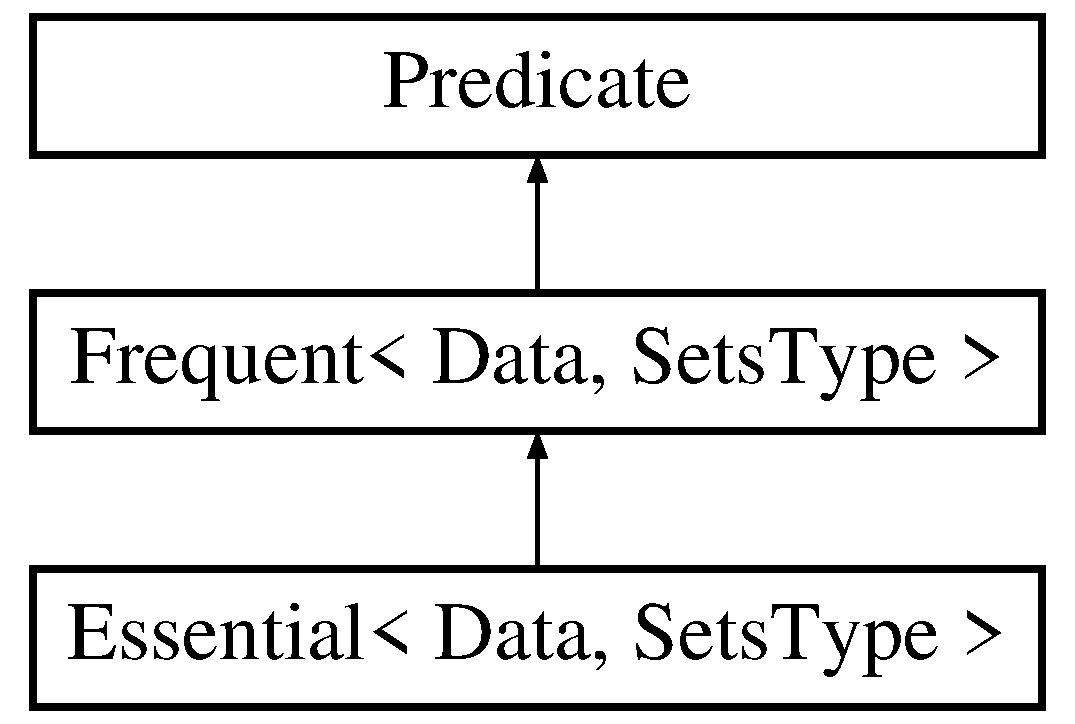
\includegraphics[height=3cm]{class_frequent}
\end{center}
\end{figure}
\subsection*{Public Member Functions}
\begin{CompactItemize}
\item 
{\bf Frequent} (Data \&indb, int in\-Minsup)
\begin{CompactList}\small\item\em Constructor. \item\end{CompactList}\item 
{\bf $\sim$Frequent} ()\label{class_frequent_c3612977fa17e8dfda09132b36a42d7f}

\begin{CompactList}\small\item\em Destructor. \item\end{CompactList}\item 
template$<$class Iterator, class Measure$>$ bool {\bf operator()} (Iterator itemset\-It, Measure \&mes\-Cand)
\begin{CompactList}\small\item\em Operator that test if an itemet is frequent or not. \item\end{CompactList}\item 
template$<$class Cand\_\-Data\-Struct, class f$>$ void {\bf pre\-Processing} (Cand\_\-Data\-Struct \&cand, f word\-To\-Set)
\begin{CompactList}\small\item\em Function used to count the support of the itemsets. \item\end{CompactList}\item 
template$<$class Cand\_\-Data\-Struct, class f$>$ void {\bf post\-Processing} (Cand\_\-Data\-Struct \&cand, f word\-To\-Set)
\begin{CompactList}\small\item\em Function used to do some post processing operations after testing the candidates generated. \item\end{CompactList}\end{CompactItemize}
\subsection*{Public Attributes}
\begin{CompactItemize}
\item 
list\-Item\-Supp {\bf list\-Item\-Support}
\begin{CompactList}\small\item\em List of all the items with their support. \item\end{CompactList}\end{CompactItemize}
\subsection*{Protected Member Functions}
\begin{CompactItemize}
\item 
template$<$class Measure, class Iterator\-Data$>$ int {\bf count} ({\bf Node}$<$ int, Measure $>$ $\ast$curr\-Node, Iterator\-Data it\-Data)
\begin{CompactList}\small\item\em Method used to count and save the support of a set of itemsets. \item\end{CompactList}\end{CompactItemize}
\subsection*{Protected Attributes}
\begin{CompactItemize}
\item 
{\bf Recode\-To\-Int}$<$ Sets\-Type $>$ {\bf recode}\label{class_frequent_3f48fefd58b3b8f45fcd4e5cc4d48931}

\begin{CompactList}\small\item\em Internal encoding of the items. \item\end{CompactList}\item 
Data $\ast$ {\bf db}\label{class_frequent_ff67dcf2a726388189b0ff9a27ef6618}

\begin{CompactList}\small\item\em The transactionnal database. \item\end{CompactList}\item 
int {\bf minsup}\label{class_frequent_23ababafb524d4f848d5e299ca2ff372}

\begin{CompactList}\small\item\em The minimum support threshold (absolute). \item\end{CompactList}\end{CompactItemize}
\subsection*{Classes}
\begin{CompactItemize}
\item 
class {\bf eq\-Item\-Supp}
\begin{CompactList}\small\item\em Functor used to find an item in the list of items/support. \item\end{CompactList}\item 
class {\bf order}
\begin{CompactList}\small\item\em Functor used to reorder a transaction. \item\end{CompactList}\item 
class {\bf reorder\-Trans}
\begin{CompactList}\small\item\em Functor that reorders a transaction and insert it in the db. \item\end{CompactList}\end{CompactItemize}


\subsection{Detailed Description}
\subsubsection*{template$<$class Data, class Sets\-Type$>$ class Frequent$<$ Data, Sets\-Type $>$}

Functor representing the predicate being frequent. 

This functor test if an itemset is frequent. This functor process the support before pruning. We suppose that the data has the same internal encoding than the candidates (ie, the first item met is recoded in \char`\"{}0\char`\"{}, the second in \char`\"{}1\char`\"{}, ...).

The methods of this predicate are specific to tries data structure ({\bf PTree}{\rm (p.\,\pageref{class_p_tree})} for the candiates and {\bf Tatree}{\rm (p.\,\pageref{class_tatree})} for the transactions). This functor cannot be used when using a transformation function (for exmaple to change the exploration of the search space).

The template parameter Data is the type of the transactional database. The template parameter Sets\-Type is the type of the items. 



\subsection{Constructor \& Destructor Documentation}
\index{Frequent@{Frequent}!Frequent@{Frequent}}
\index{Frequent@{Frequent}!Frequent@{Frequent}}
\subsubsection{\setlength{\rightskip}{0pt plus 5cm}template$<$class Data, class Sets\-Type$>$ {\bf Frequent}$<$ Data, Sets\-Type $>$::{\bf Frequent} (Data \& {\em indb}, int {\em in\-Minsup})\hspace{0.3cm}{\tt  [inline]}}\label{class_frequent_d4786ab80688426419495d0d8ff3ea47}


Constructor. 

\begin{Desc}
\item[Parameters:]
\begin{description}
\item[{\em indb}]the transactional database \item[{\em in\-Minsup}]the absolute minimum support threshold \end{description}
\end{Desc}


\subsection{Member Function Documentation}
\index{Frequent@{Frequent}!count@{count}}
\index{count@{count}!Frequent@{Frequent}}
\subsubsection{\setlength{\rightskip}{0pt plus 5cm}template$<$class Data, class Sets\-Type$>$ template$<$class Measure, class Iterator\-Data$>$ int {\bf Frequent}$<$ Data, Sets\-Type $>$::count ({\bf Node}$<$ int, Measure $>$ $\ast$ {\em curr\-Node}, Iterator\-Data {\em it\-Data})\hspace{0.3cm}{\tt  [protected]}}\label{class_frequent_50001a78dd15b91872285556ba7dfbe4}


Method used to count and save the support of a set of itemsets. 

\begin{Desc}
\item[Parameters:]
\begin{description}
\item[{\em curr\-Node}]curent node of the trie storing the itemsets \item[{\em it\-Data}]iterator on the data \end{description}
\end{Desc}
\index{Frequent@{Frequent}!operator()@{operator()}}
\index{operator()@{operator()}!Frequent@{Frequent}}
\subsubsection{\setlength{\rightskip}{0pt plus 5cm}template$<$class Data, class Sets\-Type$>$ template$<$class Iterator, class Measure$>$ bool {\bf Frequent}$<$ Data, Sets\-Type $>$::operator() (Iterator {\em itemset\-It}, Measure \& {\em mes\-Cand})\hspace{0.3cm}{\tt  [inline]}}\label{class_frequent_82e02ab1cf1749ea52e9603dc06a5d15}


Operator that test if an itemet is frequent or not. 

\begin{Desc}
\item[Parameters:]
\begin{description}
\item[{\em itemset\-It}]iterator (or pointer) on the itemset to test wrt the predicate \item[{\em mes\-Cand}]value of the support of the itemset \end{description}
\end{Desc}


Reimplemented from {\bf Predicate} {\rm (p.\,\pageref{class_predicate_6fb1a75dba2268f75738f335f403e46c})}.

Reimplemented in {\bf Essential$<$ Data, Sets\-Type $>$} {\rm (p.\,\pageref{class_essential_e6a89fa2543fe441619066b0f4f6323b})}.\index{Frequent@{Frequent}!postProcessing@{postProcessing}}
\index{postProcessing@{postProcessing}!Frequent@{Frequent}}
\subsubsection{\setlength{\rightskip}{0pt plus 5cm}template$<$class Data, class Sets\-Type$>$ template$<$class Cand\_\-Data\-Struct, class f$>$ void {\bf Frequent}$<$ Data, Sets\-Type $>$::post\-Processing (Cand\_\-Data\-Struct \& {\em cand}, f {\em word\-To\-Set})}\label{class_frequent_ff29167beb828195c34e10881abb2f74}


Function used to do some post processing operations after testing the candidates generated. 

Method used to reconstruct the db after discovery of frequent items. Prune from the transactions all the not frequent items. \begin{Desc}
\item[Parameters:]
\begin{description}
\item[{\em cand}]container of words of the language. \item[{\em word\-Toset}]functor that eventually transforms itemsets \end{description}
\end{Desc}


Reimplemented from {\bf Predicate} {\rm (p.\,\pageref{class_predicate_49f7acb334fac851a26a4d1aecc64571})}.\index{Frequent@{Frequent}!preProcessing@{preProcessing}}
\index{preProcessing@{preProcessing}!Frequent@{Frequent}}
\subsubsection{\setlength{\rightskip}{0pt plus 5cm}template$<$class Data, class Sets\-Type$>$ template$<$class Cand\_\-Data\-Struct, class f$>$ void {\bf Frequent}$<$ Data, Sets\-Type $>$::pre\-Processing (Cand\_\-Data\-Struct \& {\em cand}, f {\em word\-To\-Set})}\label{class_frequent_236bb06ebfac503436c8a25a8507b467}


Function used to count the support of the itemsets. 

Method used to count the support of itemsets. For each transaction of the db update the supports of all the itemsets in cand. \begin{Desc}
\item[Parameters:]
\begin{description}
\item[{\em cand}]container of words of the language. \item[{\em word\-Toset}]functor that eventually transforms itemsets \end{description}
\end{Desc}


Reimplemented from {\bf Predicate} {\rm (p.\,\pageref{class_predicate_8ee59d790e9b46e5e0555dbeb5b91f95})}.

\subsection{Member Data Documentation}
\index{Frequent@{Frequent}!listItemSupport@{listItemSupport}}
\index{listItemSupport@{listItemSupport}!Frequent@{Frequent}}
\subsubsection{\setlength{\rightskip}{0pt plus 5cm}template$<$class Data, class Sets\-Type$>$ list\-Item\-Supp {\bf Frequent}$<$ Data, Sets\-Type $>$::{\bf list\-Item\-Support}}\label{class_frequent_5eee2b41720ffc388e3863f54c62624f}


List of all the items with their support. 

Used to avoid support counting for items since in the initialization functor the items support is processed. Set in the initialization functor. 

The documentation for this class was generated from the following file:\begin{CompactItemize}
\item 
F:/i\-Zi/problems/frequent/Frequent.hxx\end{CompactItemize}

\section{Frequent$<$ Data, Sets\-Type $>$::eq\-Item\-Supp Class Reference}
\label{class_frequent_1_1eq_item_supp}\index{Frequent::eqItemSupp@{Frequent::eqItemSupp}}
Functor used to find an item in the list of items/support.  


{\tt \#include $<$Frequent.hxx$>$}



\subsection{Detailed Description}
\subsubsection*{template$<$class Data, class Sets\-Type$>$ class Frequent$<$ Data, Sets\-Type $>$::eq\-Item\-Supp}

Functor used to find an item in the list of items/support. 



The documentation for this class was generated from the following file:\begin{CompactItemize}
\item 
F:/i\-Zi/problems/frequent/Frequent.hxx\end{CompactItemize}

\section{Frequent$<$ Data, Sets\-Type $>$::order Class Reference}
\label{class_frequent_1_1order}\index{Frequent::order@{Frequent::order}}
Functor used to reorder a transaction.  


{\tt \#include $<$Frequent.hxx$>$}



\subsection{Detailed Description}
\subsubsection*{template$<$class Data, class Sets\-Type$>$ class Frequent$<$ Data, Sets\-Type $>$::order}

Functor used to reorder a transaction. 



The documentation for this class was generated from the following file:\begin{CompactItemize}
\item 
F:/i\-Zi/problems/frequent/Frequent.hxx\end{CompactItemize}

\section{Frequent$<$ Data, Sets\-Type $>$::reorder\-Trans Class Reference}
\label{class_frequent_1_1reorder_trans}\index{Frequent::reorderTrans@{Frequent::reorderTrans}}
Functor that reorders a transaction and insert it in the db.  


{\tt \#include $<$Frequent.hxx$>$}

\subsection*{Public Member Functions}
\begin{CompactItemize}
\item 
{\bf reorder\-Trans} (Data $\ast$indb, int nbfreq, {\bf Recode\-To\-Int}$<$ Sets\-Type $>$ $\ast$inrecode)\label{class_frequent_1_1reorder_trans_4c3ec352fdc134b0f8abbe059fbd6fef}

\begin{CompactList}\small\item\em Contructor. \item\end{CompactList}\item 
{\bf $\sim$reorder\-Trans} ()\label{class_frequent_1_1reorder_trans_26d0f52720ada6108cc16ddfdb5c3899}

\begin{CompactList}\small\item\em Destructor. \item\end{CompactList}\end{CompactItemize}


\subsection{Detailed Description}
\subsubsection*{template$<$class Data, class Sets\-Type$>$ class Frequent$<$ Data, Sets\-Type $>$::reorder\-Trans}

Functor that reorders a transaction and insert it in the db. 

The template parameter {\bf Binary\-DB}{\rm (p.\,\pageref{class_binary_d_b})} is the class representing the bianry database 



The documentation for this class was generated from the following file:\begin{CompactItemize}
\item 
F:/i\-Zi/problems/frequent/Frequent.hxx\end{CompactItemize}

\section{Id Class Reference}
\label{class_id}\index{Id@{Id}}
Functor that represents identity function.  


{\tt \#include $<$Id.hpp$>$}

\subsection*{Public Member Functions}
\begin{CompactItemize}
\item 
template$<$class Iterator\-Set$>$ Iterator\-Set {\bf operator()} (Iterator\-Set s)\label{class_id_7aea166dc5d92a9f25a2f27bde72898d}

\begin{CompactList}\small\item\em Operator returning the identity. \item\end{CompactList}\item 
template$<$class Iterator\-Set$>$ Iterator\-Set {\bf inverse} (Iterator\-Set s)\label{class_id_a1bfcb19aff95428c2f8ec4ea8043eea}

\begin{CompactList}\small\item\em Method returning the identity. \item\end{CompactList}\end{CompactItemize}


\subsection{Detailed Description}
Functor that represents identity function. 



The documentation for this class was generated from the following file:\begin{CompactItemize}
\item 
F:/i\-Zi/algorithms/Id.hpp\end{CompactItemize}

\section{IND Class Reference}
\label{class_i_n_d}\index{IND@{IND}}
Class representing a {\bf IND}{\rm (p.\,\pageref{class_i_n_d})}.  


{\tt \#include $<$IND.hpp$>$}

\subsection*{Public Member Functions}
\begin{CompactItemize}
\item 
int {\bf size} ()\label{class_i_n_d_b18ab142c3d20be97b0782b568c8a2a6}

\begin{CompactList}\small\item\em Return the size of the {\bf IND}{\rm (p.\,\pageref{class_i_n_d})}. \item\end{CompactList}\end{CompactItemize}
\subsection*{Public Attributes}
\begin{CompactItemize}
\item 
vector$<$ string $>$ {\bf left}\label{class_i_n_d_0fd6f015101c07bf3e59108d5d62a7c8}

\begin{CompactList}\small\item\em left side of the {\bf IND}{\rm (p.\,\pageref{class_i_n_d})} \item\end{CompactList}\item 
vector$<$ string $>$ {\bf right}\label{class_i_n_d_e9bcd3588ce512c15c5cf0a618402154}

\begin{CompactList}\small\item\em right side of the {\bf IND}{\rm (p.\,\pageref{class_i_n_d})} \item\end{CompactList}\end{CompactItemize}


\subsection{Detailed Description}
Class representing a {\bf IND}{\rm (p.\,\pageref{class_i_n_d})}. 



The documentation for this class was generated from the following file:\begin{CompactItemize}
\item 
F:/i\-Zi/problems/DI/IND.hpp\end{CompactItemize}

\section{Init\-Frequent$<$ Sets\-Type, Binary\-DB, Predicate $>$ Class Template Reference}
\label{class_init_frequent}\index{InitFrequent@{InitFrequent}}
Functor used to initialize the frequent items.  


{\tt \#include $<$Init\-Frequent.hxx$>$}

\subsection*{Public Member Functions}
\begin{CompactItemize}
\item 
{\bf Init\-Frequent} ({\bf Binary\-DB} \&indb, {\bf Predicate} \&inpred)\label{class_init_frequent_686b379a23f75c8e1df5c8702d462683}

\begin{CompactList}\small\item\em Constructor. \item\end{CompactList}\item 
void {\bf operator()} ()\label{class_init_frequent_8f248a5ae7603efb1b9bc52ff7323bbd}

\begin{CompactList}\small\item\em Operator excuting this initialization function in the algorithm. \item\end{CompactList}\end{CompactItemize}
\subsection*{Public Attributes}
\begin{CompactItemize}
\item 
deque$<$ Sets\-Type $>$ {\bf list\-Elements}\label{class_init_frequent_7bbf538d239ba565980cd201b7b5f08a}

\begin{CompactList}\small\item\em List of the items. \item\end{CompactList}\end{CompactItemize}
\subsection*{Protected Attributes}
\begin{CompactItemize}
\item 
{\bf Binary\-DB} $\ast$ {\bf db}\label{class_init_frequent_86b635685b8d2a731805f276541a0985}

\begin{CompactList}\small\item\em The database. \item\end{CompactList}\item 
{\bf Predicate} $\ast$ {\bf pred}\label{class_init_frequent_5e3ffe3b474496e68eea25682e1f7f0b}

\begin{CompactList}\small\item\em The predicate. \item\end{CompactList}\end{CompactItemize}


\subsection{Detailed Description}
\subsubsection*{template$<$class Sets\-Type, class Binary\-DB, class Predicate$>$ class Init\-Frequent$<$ Sets\-Type, Binary\-DB, Predicate $>$}

Functor used to initialize the frequent items. 

This functor is used to search the items in the database with their support. It is passed in parameter of the algorithms and execute int the algorithm.

The predicate is used in this class to store the items with their support.

The template parameter Sets\-Type is the type of the items. The template parameter {\bf Binary\-DB}{\rm (p.\,\pageref{class_binary_d_b})} is the type of the transactional database. The template parameter {\bf Predicate}{\rm (p.\,\pageref{class_predicate})} is the type of the predicate used to select interesting items. 



The documentation for this class was generated from the following file:\begin{CompactItemize}
\item 
F:/i\-Zi/problems/frequent/Init\-Frequent.hxx\end{CompactItemize}

\section{Init\-IND$<$ Input\-DBFormat $>$ Class Template Reference}
\label{class_init_i_n_d}\index{InitIND@{InitIND}}
Functor used to intialize the {\bf IND}{\rm (p.\,\pageref{class_i_n_d})} mining.  


{\tt \#include $<$Init\-IND.hxx$>$}

\subsection*{Public Member Functions}
\begin{CompactItemize}
\item 
{\bf Init\-IND} (Input\-DBFormat \&ininput1, Input\-DBFormat \&ininput2)\label{class_init_i_n_d_5fa698ef8b2c267a5d2c4883a7065604}

\begin{CompactList}\small\item\em Constructor. \item\end{CompactList}\item 
void {\bf operator()} ()\label{class_init_i_n_d_f9c79264f50185ebfecaf071b1021411}

\begin{CompactList}\small\item\em Execute the initialization of the basic word of the language (the di of size 1) in the algorithm. \item\end{CompactList}\end{CompactItemize}
\subsection*{Public Attributes}
\begin{CompactItemize}
\item 
deque$<$ {\bf IND} $>$ {\bf list\-Elements}\label{class_init_i_n_d_3eca6bee3e17f420c62bd89edd5c06c5}

\begin{CompactList}\small\item\em list of the unary {\bf IND}{\rm (p.\,\pageref{class_i_n_d})} \item\end{CompactList}\end{CompactItemize}
\subsection*{Protected Attributes}
\begin{CompactItemize}
\item 
Input\-DBFormat $\ast$ {\bf input1}\label{class_init_i_n_d_88db2dbdbc7fe5e373e386583e1ed0cb}

\begin{CompactList}\small\item\em The first input relational data. \item\end{CompactList}\item 
Input\-DBFormat $\ast$ {\bf input2}\label{class_init_i_n_d_29f5e69e0cb428a4bcccf69b63331294}

\begin{CompactList}\small\item\em The second input relational data. \item\end{CompactList}\end{CompactItemize}


\subsection{Detailed Description}
\subsubsection*{template$<$class Input\-DBFormat$>$ class Init\-IND$<$ Input\-DBFormat $>$}

Functor used to intialize the {\bf IND}{\rm (p.\,\pageref{class_i_n_d})} mining. 

This functor is used to search the attributes of the relations and to construct the initial set unary INDs.

The template parameter Input\-DBFormat is the type of the database. 



The documentation for this class was generated from the following file:\begin{CompactItemize}
\item 
F:/i\-Zi/problems/DI/Init\-IND.hxx\end{CompactItemize}

\section{Init\-IND\_\-DBMS$<$ DBMS $>$ Class Template Reference}
\label{class_init_i_n_d___d_b_m_s}\index{InitIND_DBMS@{InitIND\_\-DBMS}}
Functor used to intialize the {\bf IND}{\rm (p.\,\pageref{class_i_n_d})} mining.  


{\tt \#include $<$Init\-IND\_\-DBMS.hxx$>$}

\subsection*{Public Member Functions}
\begin{CompactItemize}
\item 
{\bf Init\-IND\_\-DBMS} (DBMS $\ast$in\-Dbms)
\begin{CompactList}\small\item\em Constructor. \item\end{CompactList}\item 
void {\bf operator()} ()\label{class_init_i_n_d___d_b_m_s_745efc71662e13dd81b11c1af3b39a28}

\begin{CompactList}\small\item\em Execute the initialization of the basic word of the language (the di of size 1) in the algorithm. \item\end{CompactList}\end{CompactItemize}
\subsection*{Public Attributes}
\begin{CompactItemize}
\item 
deque$<$ {\bf IND} $>$ {\bf list\-Elements}\label{class_init_i_n_d___d_b_m_s_58b846134793297ec3c99fa773c1d6d8}

\begin{CompactList}\small\item\em list of the unary {\bf IND}{\rm (p.\,\pageref{class_i_n_d})} \item\end{CompactList}\end{CompactItemize}
\subsection*{Protected Attributes}
\begin{CompactItemize}
\item 
DBMS $\ast$ {\bf mydbms}\label{class_init_i_n_d___d_b_m_s_a63c8d8ea2a044779d5cc55750e2fab3}

\begin{CompactList}\small\item\em Pointer on the dbms. \item\end{CompactList}\end{CompactItemize}


\subsection{Detailed Description}
\subsubsection*{template$<$class DBMS$>$ class Init\-IND\_\-DBMS$<$ DBMS $>$}

Functor used to intialize the {\bf IND}{\rm (p.\,\pageref{class_i_n_d})} mining. 

This functor is used to search the attributes of the relations and to construct the initial set unary INDs.

The template parameter DBMS is the class representing the connection to the DBMS. This class is used to do operations on the DBMS such as connect, execute a query ... 



\subsection{Constructor \& Destructor Documentation}
\index{InitIND_DBMS@{Init\-IND\_\-DBMS}!InitIND_DBMS@{InitIND\_\-DBMS}}
\index{InitIND_DBMS@{InitIND\_\-DBMS}!InitIND_DBMS@{Init\-IND\_\-DBMS}}
\subsubsection{\setlength{\rightskip}{0pt plus 5cm}template$<$class DBMS$>$ {\bf Init\-IND\_\-DBMS}$<$ DBMS $>$::{\bf Init\-IND\_\-DBMS} (DBMS $\ast$ {\em in\-Dbms})\hspace{0.3cm}{\tt  [inline]}}\label{class_init_i_n_d___d_b_m_s_fabad477760e0e4d049afba904f5388c}


Constructor. 

\begin{Desc}
\item[Parameters:]
\begin{description}
\item[{\em in\-Dbms}]pointer on the DBMS object to consider \end{description}
\end{Desc}


The documentation for this class was generated from the following file:\begin{CompactItemize}
\item 
F:/i\-Zi/problems/DI/Init\-IND\_\-DBMS.hxx\end{CompactItemize}

\section{Init\-Key$<$ Attribute\-Type, Input\-DBFormat $>$ Class Template Reference}
\label{class_init_key}\index{InitKey@{InitKey}}
Functor used to intialize the not redundant mining.  


{\tt \#include $<$Init\-Key.hxx$>$}

\subsection*{Public Member Functions}
\begin{CompactItemize}
\item 
{\bf Init\-Key} (Input\-DBFormat \&ininput)\label{class_init_key_98e5ce76e2211fa750dfdff4e61605d8}

\begin{CompactList}\small\item\em Constructor. \item\end{CompactList}\item 
void {\bf operator()} ()\label{class_init_key_0d4c102edccfdf37f747b02ed159e0c6}

\begin{CompactList}\small\item\em Execute the initialization of the basic word of the language in tha algorithm. \item\end{CompactList}\end{CompactItemize}
\subsection*{Public Attributes}
\begin{CompactItemize}
\item 
deque$<$ Attribute\-Type $>$ {\bf list\-Elements}\label{class_init_key_53242d2f0e4257b05f91e1b1f8849b4c}

\begin{CompactList}\small\item\em list of the attributes \item\end{CompactList}\end{CompactItemize}
\subsection*{Protected Attributes}
\begin{CompactItemize}
\item 
Input\-DBFormat $\ast$ {\bf input}\label{class_init_key_0c035f6bf918ef2654e40bf7a70f5a0a}

\begin{CompactList}\small\item\em The input relational data. \item\end{CompactList}\end{CompactItemize}


\subsection{Detailed Description}
\subsubsection*{template$<$class Attribute\-Type, class Input\-DBFormat$>$ class Init\-Key$<$ Attribute\-Type, Input\-DBFormat $>$}

Functor used to intialize the not redundant mining. 

This functor is used to search the attributes of the database.

The template parameter Attribute\-Type is the type of the attributes. The template parameter Input\-DBFormat is the type of the database. 



The documentation for this class was generated from the following file:\begin{CompactItemize}
\item 
F:/i\-Zi/problems/key/Init\-Key.hxx\end{CompactItemize}

\section{Is\-Almost\-Freq Class Reference}
\label{class_is_almost_freq}\index{IsAlmostFreq@{IsAlmostFreq}}
Determine if a not frequent itemset is near the positive border in the ABS algorithm.  


{\tt \#include $<$Is\-Almost\-Freq.hxx$>$}

\subsection*{Public Member Functions}
\begin{CompactItemize}
\item 
{\bf Is\-Almost\-Freq} (int inminsup, double inepsilon)\label{class_is_almost_freq_7103fd70890d938354573f4daec7e0ec}

\begin{CompactList}\small\item\em Constructor. \item\end{CompactList}\item 
template$<$class Iterator$>$ bool {\bf operator()} (Iterator it\-Elem)
\begin{CompactList}\small\item\em Determine if a not frequent itemset is \char`\"{}near\char`\"{} the positive border. \item\end{CompactList}\end{CompactItemize}
\subsection*{Protected Attributes}
\begin{CompactItemize}
\item 
double {\bf epsilon}\label{class_is_almost_freq_b6f988eaf3645c85e54dfc34e7461e64}

\begin{CompactList}\small\item\em threshold used to determine when an element is \char`\"{}near\char`\"{} the positive border \item\end{CompactList}\item 
int {\bf minsup}\label{class_is_almost_freq_94fe99251edd3b41cb4d1c6a231bd452}

\begin{CompactList}\small\item\em Minimum support thresold. \item\end{CompactList}\end{CompactItemize}


\subsection{Detailed Description}
Determine if a not frequent itemset is near the positive border in the ABS algorithm. 

In ABS, elements near the positive border are considered as frequent until the end of algorithm. The these \char`\"{}almost frequent\char`\"{} elements are used to find the underling elements of the positive border. 



\subsection{Member Function Documentation}
\index{IsAlmostFreq@{Is\-Almost\-Freq}!operator()@{operator()}}
\index{operator()@{operator()}!IsAlmostFreq@{Is\-Almost\-Freq}}
\subsubsection{\setlength{\rightskip}{0pt plus 5cm}template$<$class Iterator$>$ bool Is\-Almost\-Freq::operator() (Iterator {\em it\-Elem})\hspace{0.3cm}{\tt  [inline]}}\label{class_is_almost_freq_aed551b7b0b631e981fbecb0090aa170}


Determine if a not frequent itemset is \char`\"{}near\char`\"{} the positive border. 

A not frequent element X is \char`\"{}near\char`\"{}, if (1 - supp( X ) /minsup $<$ thresold \begin{Desc}
\item[Parameters:]
\begin{description}
\item[{\em it\-Element}]iterator on the element to study \end{description}
\end{Desc}


The documentation for this class was generated from the following file:\begin{CompactItemize}
\item 
F:/i\-Zi/problems/frequent/Is\-Almost\-Freq.hxx\end{CompactItemize}

\section{It\-Binary\-DB$<$ Sets\-Type, Data\-Struct\-DB, Container $>$ Class Template Reference}
\label{class_it_binary_d_b}\index{ItBinaryDB@{ItBinaryDB}}
Iterator on a {\bf Binary\-DB}{\rm (p.\,\pageref{class_binary_d_b})}.  


{\tt \#include $<$It\-Binary\-DB.hxx$>$}

\subsection*{Public Member Functions}
\begin{CompactItemize}
\item 
{\bf It\-Binary\-DB} ({\bf Binary\-DB}$<$ Sets\-Type, Data\-Struct\-DB $>$ $\ast$indb=0)
\begin{CompactList}\small\item\em Contructor. \item\end{CompactList}\item 
{\bf It\-Binary\-DB} (const {\bf It\-Binary\-DB} \&it)\label{class_it_binary_d_b_61f089507fe6f0a87faf85b1998f2be7}

\begin{CompactList}\small\item\em Copy contructor. \item\end{CompactList}\item 
{\bf It\-Binary\-DB} \& {\bf operator=} (const {\bf It\-Binary\-DB} \&it)\label{class_it_binary_d_b_1e9d36966f7fb7419e1902664eace7c9}

\begin{CompactList}\small\item\em Affectation operator. \item\end{CompactList}\item 
{\bf $\sim$It\-Binary\-DB} ()\label{class_it_binary_d_b_cad2c6eb1c50686997e3b2946f082243}

\begin{CompactList}\small\item\em Destructor. \item\end{CompactList}\item 
{\bf It\-Binary\-DB} \& {\bf operator++} ()
\begin{CompactList}\small\item\em Increment operator. \item\end{CompactList}\item 
{\bf It\-Binary\-DB} {\bf operator++} (int)
\begin{CompactList}\small\item\em Increment operator. \item\end{CompactList}\item 
Container \& {\bf operator $\ast$} ()\label{class_it_binary_d_b_c117c52f125ee39ef6031829ad79f79b}

\begin{CompactList}\small\item\em Operator returning the transaction pointed by the current iterator. \item\end{CompactList}\item 
Container $\ast$ {\bf operator $\rightarrow$ } ()\label{class_it_binary_d_b_1894f39ef8dff3081bfa42605fc128c1}

\begin{CompactList}\small\item\em Operator returning a pointer on the transaction pointed by the current iterator. \item\end{CompactList}\item 
bool {\bf operator==} (const {\bf It\-Binary\-DB} \&it) const \label{class_it_binary_d_b_91eafdf30203a18baf6d392a38f96b0d}

\begin{CompactList}\small\item\em Equality operator. \item\end{CompactList}\item 
bool {\bf operator!=} (const {\bf It\-Binary\-DB} \&it) const \label{class_it_binary_d_b_941afddd8f5ef0c8e0ef9370c2d85035}

\begin{CompactList}\small\item\em Difference operator. \item\end{CompactList}\end{CompactItemize}
\subsection*{Protected Attributes}
\begin{CompactItemize}
\item 
Iterator\-Data\-Struct {\bf current\-It}\label{class_it_binary_d_b_5885f783eeca530fa2f5d8f4ca772e7c}

\begin{CompactList}\small\item\em Iterator on the current transaction. \item\end{CompactList}\item 
It\-Vect\-Vect $\ast$ {\bf i\-Ttmp\-DB}\label{class_it_binary_d_b_768d3ac84d56e4c06c9d8aa72384dfd8}

\begin{CompactList}\small\item\em Iterator on the temporary db. \item\end{CompactList}\item 
Iterator\-Data\-Struct {\bf end\-It}\label{class_it_binary_d_b_5444ed214330550b28da30032caa76d4}

\begin{CompactList}\small\item\em Iterator on the end of thetransaction. \item\end{CompactList}\item 
It\-Vect\-Vect $\ast$ {\bf end\-It\-Tmp}\label{class_it_binary_d_b_99d05794ac53f0479a1dacd03dd74fc0}

\begin{CompactList}\small\item\em Iterator on the end of the temporary db. \item\end{CompactList}\end{CompactItemize}
\subsection*{Friends}
\begin{CompactItemize}
\item 
class {\bf Binary\-DB$<$ Sets\-Type, Data\-Struct\-DB $>$}\label{class_it_binary_d_b_040243f5590d2e87774acbc72e24382d}

\end{CompactItemize}


\subsection{Detailed Description}
\subsubsection*{template$<$class Sets\-Type, class Data\-Struct\-DB, class Container = vector$<$Sets\-Type$>$$>$ class It\-Binary\-DB$<$ Sets\-Type, Data\-Struct\-DB, Container $>$}

Iterator on a {\bf Binary\-DB}{\rm (p.\,\pageref{class_binary_d_b})}. 

The template parameter Sets\-Type is the type of the element stored in the db. The template parameter Data\-Struct\-DB is the type of the data structure storing the db. The template parameter Container is the container used to store the transactions.

\begin{Desc}
\item[See also:]{\bf Binary\-DB}{\rm (p.\,\pageref{class_binary_d_b})}. \end{Desc}




\subsection{Constructor \& Destructor Documentation}
\index{ItBinaryDB@{It\-Binary\-DB}!ItBinaryDB@{ItBinaryDB}}
\index{ItBinaryDB@{ItBinaryDB}!ItBinaryDB@{It\-Binary\-DB}}
\subsubsection{\setlength{\rightskip}{0pt plus 5cm}template$<$class Sets\-Type, class Data\-Struct\-DB, class Container = vector$<$Sets\-Type$>$$>$ {\bf It\-Binary\-DB}$<$ Sets\-Type, Data\-Struct\-DB, Container $>$::{\bf It\-Binary\-DB} ({\bf Binary\-DB}$<$ Sets\-Type, Data\-Struct\-DB $>$ $\ast$ {\em indb} = {\tt 0})\hspace{0.3cm}{\tt  [inline]}}\label{class_it_binary_d_b_79ec8ddfa713a15b83ed1ee55de9a4cb}


Contructor. 

Initialize the iterators on the db or in the temporary db if the final does not exist. 

\subsection{Member Function Documentation}
\index{ItBinaryDB@{It\-Binary\-DB}!operator++@{operator++}}
\index{operator++@{operator++}!ItBinaryDB@{It\-Binary\-DB}}
\subsubsection{\setlength{\rightskip}{0pt plus 5cm}template$<$class Sets\-Type, class Data\-Struct\-DB, class Container = vector$<$Sets\-Type$>$$>$ {\bf It\-Binary\-DB} {\bf It\-Binary\-DB}$<$ Sets\-Type, Data\-Struct\-DB, Container $>$::operator++ (int)\hspace{0.3cm}{\tt  [inline]}}\label{class_it_binary_d_b_85521883adc83343d2e3b0ce82ef1adc}


Increment operator. 

get the next set stored. \index{ItBinaryDB@{It\-Binary\-DB}!operator++@{operator++}}
\index{operator++@{operator++}!ItBinaryDB@{It\-Binary\-DB}}
\subsubsection{\setlength{\rightskip}{0pt plus 5cm}template$<$class Sets\-Type, class Data\-Struct\-DB, class Container = vector$<$Sets\-Type$>$$>$ {\bf It\-Binary\-DB}\& {\bf It\-Binary\-DB}$<$ Sets\-Type, Data\-Struct\-DB, Container $>$::operator++ ()\hspace{0.3cm}{\tt  [inline]}}\label{class_it_binary_d_b_b3ebf157e20f4fc8a4fca5172e469210}


Increment operator. 

get the next set stored. 

The documentation for this class was generated from the following file:\begin{CompactItemize}
\item 
F:/i\-Zi/data/memory/It\-Binary\-DB.hxx\end{CompactItemize}

\section{It\-Fimi\-File$<$ Sets\-Type $>$ Class Template Reference}
\label{class_it_fimi_file}\index{ItFimiFile@{ItFimiFile}}
Iterator on a {\bf Fimi\-File}{\rm (p.\,\pageref{class_fimi_file})}.  


{\tt \#include $<$It\-Fimi\-File.hxx$>$}

\subsection*{Public Member Functions}
\begin{CompactItemize}
\item 
{\bf It\-Fimi\-File} ({\bf Fimi\-File}$<$ Sets\-Type $>$ $\ast$ffile=0)\label{class_it_fimi_file_e1f80f41516c1e0cc918f97e11b5e80d}

\begin{CompactList}\small\item\em Contructor. \item\end{CompactList}\item 
{\bf It\-Fimi\-File} (const {\bf It\-Fimi\-File} \&it)\label{class_it_fimi_file_c59e024aa9b426be7648fc2282b5a823}

\begin{CompactList}\small\item\em Copy contructor. \item\end{CompactList}\item 
{\bf It\-Fimi\-File} \& {\bf operator=} (const {\bf It\-Fimi\-File} \&it)\label{class_it_fimi_file_16c6213b3f03462beef7ba5d98e29975}

\begin{CompactList}\small\item\em Affectation operator. \item\end{CompactList}\item 
{\bf $\sim$It\-Fimi\-File} ()\label{class_it_fimi_file_c8d5eb337118f5d15a6ba67611641127}

\begin{CompactList}\small\item\em Destructor. \item\end{CompactList}\item 
{\bf It\-Fimi\-File} \& {\bf operator++} ()
\begin{CompactList}\small\item\em Increment operator. \item\end{CompactList}\item 
{\bf It\-Fimi\-File} {\bf operator++} (int)
\begin{CompactList}\small\item\em Increment operator. \item\end{CompactList}\item 
vector$<$ Sets\-Type $>$ \& {\bf operator $\ast$} ()\label{class_it_fimi_file_26e22a0dbc9b37fc0dd36b0a4fa1d0e0}

\begin{CompactList}\small\item\em Operator returing the transaction pointed by the iterator. \item\end{CompactList}\item 
vector$<$ Sets\-Type $>$ $\ast$ {\bf operator $\rightarrow$ } ()\label{class_it_fimi_file_f5dce33c2c37373cfb09595d601b9180}

\begin{CompactList}\small\item\em Operator returing a pointer on the transaction pointed by the iterator. \item\end{CompactList}\item 
bool {\bf operator==} (const {\bf It\-Fimi\-File} \&it) const \label{class_it_fimi_file_ec245aaf60f7889a07fbaba20c77be51}

\begin{CompactList}\small\item\em Equality operator. \item\end{CompactList}\item 
bool {\bf operator!=} (const {\bf It\-Fimi\-File} \&it) const \label{class_it_fimi_file_29c9d50f9de562927c85aeac944d46cf}

\begin{CompactList}\small\item\em Difference operator. \item\end{CompactList}\end{CompactItemize}
\subsection*{Protected Attributes}
\begin{CompactItemize}
\item 
{\bf Fimi\-File}$<$ Sets\-Type $>$ $\ast$ {\bf fimi\-File}\label{class_it_fimi_file_9edb330d528dd195a9170c109e89c425}

\begin{CompactList}\small\item\em current {\bf Fimi\-File}{\rm (p.\,\pageref{class_fimi_file})} \item\end{CompactList}\item 
vector$<$ Sets\-Type $>$ {\bf current\-Data}\label{class_it_fimi_file_57d6d5ca0a559b25e5f53a236eb40942}

\begin{CompactList}\small\item\em container with the current Data. \item\end{CompactList}\end{CompactItemize}
\subsection*{Friends}
\begin{CompactItemize}
\item 
class {\bf Fimi\-File$<$ Sets\-Type $>$}\label{class_it_fimi_file_26481749a1d5964abcc437208e9c1013}

\end{CompactItemize}


\subsection{Detailed Description}
\subsubsection*{template$<$class Sets\-Type = int$>$ class It\-Fimi\-File$<$ Sets\-Type $>$}

Iterator on a {\bf Fimi\-File}{\rm (p.\,\pageref{class_fimi_file})}. 

The template parameter Container is the container use to store the data. \begin{Desc}
\item[See also:]{\bf Fimi\-File}{\rm (p.\,\pageref{class_fimi_file})}. \end{Desc}




\subsection{Member Function Documentation}
\index{ItFimiFile@{It\-Fimi\-File}!operator++@{operator++}}
\index{operator++@{operator++}!ItFimiFile@{It\-Fimi\-File}}
\subsubsection{\setlength{\rightskip}{0pt plus 5cm}template$<$class Sets\-Type = int$>$ {\bf It\-Fimi\-File} {\bf It\-Fimi\-File}$<$ Sets\-Type $>$::operator++ (int)\hspace{0.3cm}{\tt  [inline]}}\label{class_it_fimi_file_44783f44e41095e7b9930a62dfc7ec12}


Increment operator. 

get the next data stored. \index{ItFimiFile@{It\-Fimi\-File}!operator++@{operator++}}
\index{operator++@{operator++}!ItFimiFile@{It\-Fimi\-File}}
\subsubsection{\setlength{\rightskip}{0pt plus 5cm}template$<$class Sets\-Type = int$>$ {\bf It\-Fimi\-File}\& {\bf It\-Fimi\-File}$<$ Sets\-Type $>$::operator++ ()\hspace{0.3cm}{\tt  [inline]}}\label{class_it_fimi_file_614bd34a7dad419043dc2ce43578beca}


Increment operator. 

get the next data stored. 

The documentation for this class was generated from the following file:\begin{CompactItemize}
\item 
F:/i\-Zi/data/file/It\-Fimi\-File.hxx\end{CompactItemize}

\section{It\-PTree$<$ Sets\-Type, Measure $>$ Class Template Reference}
\label{class_it_p_tree}\index{ItPTree@{ItPTree}}
Iterator on a {\bf PTree}{\rm (p.\,\pageref{class_p_tree})} (trie data structure).  


{\tt \#include $<$It\-PTree.hxx$>$}

\subsection*{Public Member Functions}
\begin{CompactItemize}
\item 
void {\bf next\-Itemset} ({\bf It\-PTree} $\ast$)\label{class_it_p_tree_00480e1f67fe1114bd8ea3811dba2c63}

\begin{CompactList}\small\item\em search the last node of the next itemset. \item\end{CompactList}\item 
void {\bf get\-Set} (vector$<$ int $>$ $\ast$inset, {\bf It\-PTree} $\ast$it)
\begin{CompactList}\small\item\em Get the set (internal id ) stored in the node pointed by the iterator passed in parameter. \item\end{CompactList}\item 
{\bf It\-PTree} ({\bf Node}$<$ Sets\-Type, Measure $>$ $\ast$currnode=0, int ininternal\-Id=0, {\bf Recode\-To\-Int}$<$ Sets\-Type $>$ $\ast$inrecode=0, int inheight=0)\label{class_it_p_tree_b45ae5524947493010acbcdc17b5889d}

\begin{CompactList}\small\item\em Default constructor. \item\end{CompactList}\item 
{\bf It\-PTree} ({\bf PTree}$<$ Sets\-Type, Measure $>$ $\ast$)\label{class_it_p_tree_794673b75fe375180e69425c1342aa46}

\begin{CompactList}\small\item\em Contructor setting the iterator on the first set of the trie. \item\end{CompactList}\item 
{\bf It\-PTree} ({\bf Node}$<$ Sets\-Type, Measure $>$ $\ast$, {\bf Recode\-To\-Int}$<$ Sets\-Type $>$ $\ast$)\label{class_it_p_tree_e31d719e378bd26422db9ef26e6e2f34}

\begin{CompactList}\small\item\em Contructor setting the iterator on the first leaf of the trie. \item\end{CompactList}\item 
{\bf It\-PTree} (const {\bf It\-PTree} \&it)\label{class_it_p_tree_117622ebdf8424515868e2de71586c6a}

\begin{CompactList}\small\item\em Copy constructor. \item\end{CompactList}\item 
{\bf It\-PTree} \& {\bf operator=} (const {\bf It\-PTree} \&it)\label{class_it_p_tree_4f4f9bf0510afd02ceae063985f4366c}

\begin{CompactList}\small\item\em Affectation operator. \item\end{CompactList}\item 
{\bf $\sim$It\-PTree} ()\label{class_it_p_tree_52ad99488e1ce902784c99f5a1b74ebb}

\begin{CompactList}\small\item\em Destructor. \item\end{CompactList}\item 
vector$<$ Sets\-Type $>$ \& {\bf operator $\ast$} ()\label{class_it_p_tree_1fd34185f8b28f6029c93142b705373c}

\begin{CompactList}\small\item\em Operator returning the current set. \item\end{CompactList}\item 
vector$<$ Sets\-Type $>$ $\ast$ {\bf operator $\rightarrow$ } ()\label{class_it_p_tree_dfd046def36cc49a70979af63d38a03a}

\begin{CompactList}\small\item\em Operator returning a pointer on the current set. \item\end{CompactList}\item 
bool {\bf operator==} (const {\bf It\-PTree} \&it) const \label{class_it_p_tree_b9077c68640add8a17995fd47157d457}

\begin{CompactList}\small\item\em Equality operator. \item\end{CompactList}\item 
bool {\bf operator!=} (const {\bf It\-PTree} \&it) const \label{class_it_p_tree_6cc6bc3ccd5755ef7a91a8b3ecd73ee5}

\begin{CompactList}\small\item\em Difference operator. \item\end{CompactList}\item 
{\bf It\-PTree} \& {\bf operator++} ()\label{class_it_p_tree_0e42ede29d18334dcedbb0656b8372a7}

\begin{CompactList}\small\item\em Move the iterator on the next set stored (not necessarely on a leaf node for subsets). \item\end{CompactList}\item 
{\bf It\-PTree} {\bf operator++} (int)\label{class_it_p_tree_92399b9aead4b4e16fc1996fa52d2e55}

\begin{CompactList}\small\item\em Move the iterator on the next set stored (not necessarely on a leaf node for subsets). \item\end{CompactList}\item 
bool {\bf isa\-Leaf} ()
\begin{CompactList}\small\item\em Function returning if the iterrator is on a leaf node. \item\end{CompactList}\item 
{\bf It\-PTree} {\bf parent\-Node} ()
\begin{CompactList}\small\item\em Return an iterator on the parent node. \item\end{CompactList}\item 
{\bf It\-PTree} {\bf child\-Node} (Sets\-Type elem)
\begin{CompactList}\small\item\em Return an iterator on a child node (of the current node) containing the element elem . \item\end{CompactList}\item 
{\bf It\-PTree} {\bf next\-Child\-Node} ()
\begin{CompactList}\small\item\em Return an iterator on the next (wrt order of elements) child node of the current parent node. \item\end{CompactList}\item 
{\bf It\-PTree} {\bf next\-Leaf} ()\label{class_it_p_tree_95240af4b79e469ec380c1b54fe817dc}

\begin{CompactList}\small\item\em Return an iterator on the next leaf (exploring the tree from the left to the right). \item\end{CompactList}\item 
{\bf It\-PTree} {\bf rnext\-Leaf} ()\label{class_it_p_tree_61d94e058defaeb91643a535052bee70}

\begin{CompactList}\small\item\em Return an iterator on the next leaf (exploring the tree from the right to the left). \item\end{CompactList}\item 
int {\bf length} ()\label{class_it_p_tree_3aebe53355c21edb34cc2e25454a3fcf}

\begin{CompactList}\small\item\em Return the depth from the root node. \item\end{CompactList}\item 
Measure \& {\bf measure} ()\label{class_it_p_tree_daea7ce1f54bb2a0a396a59760eb395b}

\begin{CompactList}\small\item\em return the measure store in the node adn associated to the set \item\end{CompactList}\item 
void {\bf measure} (Measure inmeasure)\label{class_it_p_tree_e9b79aec7d04e65744343f3048abc372}

\begin{CompactList}\small\item\em return the measure store in the node adn associated to the set \item\end{CompactList}\item 
Sets\-Type {\bf element} ()\label{class_it_p_tree_df77aafe855d6c921977ecc2f5388f77}

\begin{CompactList}\small\item\em Function returning the element in the current node. \item\end{CompactList}\item 
int {\bf element\-Id} ()\label{class_it_p_tree_284b2f920da52b668a18aa6b12f5ec34}

\begin{CompactList}\small\item\em Function returning the internal id of the element in the current node. \item\end{CompactList}\item 
{\bf Node}$<$ Sets\-Type, Measure $>$ $\ast$ {\bf node} ()\label{class_it_p_tree_5633f67ecb2d18f15f8142a569cf407c}

\begin{CompactList}\small\item\em return a pointer on the current node \item\end{CompactList}\item 
vector$<$ int $>$ $\ast$ {\bf get\-Internalset} ()\label{class_it_p_tree_c13f15dd60dbc7f8a82214a49b8fc327}

\begin{CompactList}\small\item\em return the current set (with internal ids) from the curent node \item\end{CompactList}\end{CompactItemize}
\subsection*{Public Attributes}
\begin{CompactItemize}
\item 
vector$<$ int $>$ $\ast$ {\bf internalset}\label{class_it_p_tree_e6950df1aac78bcbe276e58e406fbc08}

\begin{CompactList}\small\item\em used for sets extraction by $\ast$ and -$>$ \item\end{CompactList}\end{CompactItemize}
\subsection*{Protected Attributes}
\begin{CompactItemize}
\item 
{\bf Node}$<$ Sets\-Type, Measure $>$ $\ast$ {\bf ptr}\label{class_it_p_tree_9f4c498657335bce50e4336cb775e729}

\begin{CompactList}\small\item\em Current {\bf Node}{\rm (p.\,\pageref{class_node})}. \item\end{CompactList}\item 
int {\bf internal\-Id}\label{class_it_p_tree_fb87b00832503526833a7d793f582f79}

\begin{CompactList}\small\item\em Internal id (an integer) of the curent element. \item\end{CompactList}\item 
{\bf Recode\-To\-Int}$<$ Sets\-Type $>$ $\ast$ {\bf recode}\label{class_it_p_tree_b6b3b71b329222db27d080d47bf8039a}

\begin{CompactList}\small\item\em {\bf Recode}{\rm (p.\,\pageref{class_recode})} the elements in integers. \item\end{CompactList}\item 
int {\bf height}\label{class_it_p_tree_967c7b9bba31e69d9e5acbc40906e3ab}

\begin{CompactList}\small\item\em Number of nodes from the root node. \item\end{CompactList}\end{CompactItemize}
\subsection*{Friends}
\begin{CompactItemize}
\item 
class {\bf Node$<$ Sets\-Type, Measure $>$}\label{class_it_p_tree_56b777f68cd8d1ed34d04e1cc4e96041}

\item 
class {\bf PTree$<$ Sets\-Type, Measure $>$}\label{class_it_p_tree_75985e4c63d08b10230ccb3b9f097182}

\end{CompactItemize}


\subsection{Detailed Description}
\subsubsection*{template$<$class Sets\-Type, class Measure = Boolean$>$ class It\-PTree$<$ Sets\-Type, Measure $>$}

Iterator on a {\bf PTree}{\rm (p.\,\pageref{class_p_tree})} (trie data structure). 

The template parameter Sets\-Type is the type of the elements stored in the trie. The template parameter Measure is the type used in the \char`\"{}boolean\char`\"{} vector to code the presence of an element. \begin{Desc}
\item[See also:]{\bf PTree}{\rm (p.\,\pageref{class_p_tree})}. \end{Desc}




\subsection{Member Function Documentation}
\index{ItPTree@{It\-PTree}!childNode@{childNode}}
\index{childNode@{childNode}!ItPTree@{It\-PTree}}
\subsubsection{\setlength{\rightskip}{0pt plus 5cm}template$<$class Sets\-Type, class Measure = Boolean$>$ {\bf It\-PTree} {\bf It\-PTree}$<$ Sets\-Type, Measure $>$::child\-Node (Sets\-Type {\em elem})\hspace{0.3cm}{\tt  [inline]}}\label{class_it_p_tree_91d6a798cefed637033d73de2ec00551}


Return an iterator on a child node (of the current node) containing the element elem . 

return the default iterator if there is no child node with the element. \index{ItPTree@{It\-PTree}!getSet@{getSet}}
\index{getSet@{getSet}!ItPTree@{It\-PTree}}
\subsubsection{\setlength{\rightskip}{0pt plus 5cm}template$<$class Sets\-Type, class Measure$>$ void {\bf It\-PTree}$<$ Sets\-Type, Measure $>$::get\-Set (vector$<$ int $>$ $\ast$ {\em inset}, {\bf It\-PTree}$<$ Sets\-Type, Measure $>$ $\ast$ {\em it})}\label{class_it_p_tree_5cb6cca573fcd5dc61612f1e42089fd0}


Get the set (internal id ) stored in the node pointed by the iterator passed in parameter. 

\begin{Desc}
\item[Parameters:]
\begin{description}
\item[{\em inset}]vector of SIZE it-$>$length where the elements are stored. \item[{\em it}]iterator on the last node storing the last element of the set to extract. \end{description}
\end{Desc}
\index{ItPTree@{It\-PTree}!isaLeaf@{isaLeaf}}
\index{isaLeaf@{isaLeaf}!ItPTree@{It\-PTree}}
\subsubsection{\setlength{\rightskip}{0pt plus 5cm}template$<$class Sets\-Type, class Measure = Boolean$>$ bool {\bf It\-PTree}$<$ Sets\-Type, Measure $>$::isa\-Leaf ()\hspace{0.3cm}{\tt  [inline]}}\label{class_it_p_tree_b47274ccede2e15f5248e94fe19b81e0}


Function returning if the iterrator is on a leaf node. 

\begin{Desc}
\item[Returns:]true if the current node is a leaf node. \end{Desc}
\index{ItPTree@{It\-PTree}!nextChildNode@{nextChildNode}}
\index{nextChildNode@{nextChildNode}!ItPTree@{It\-PTree}}
\subsubsection{\setlength{\rightskip}{0pt plus 5cm}template$<$class Sets\-Type, class Measure = Boolean$>$ {\bf It\-PTree} {\bf It\-PTree}$<$ Sets\-Type, Measure $>$::next\-Child\-Node ()\hspace{0.3cm}{\tt  [inline]}}\label{class_it_p_tree_393c897eec99dd8c5aaac7bf76b61733}


Return an iterator on the next (wrt order of elements) child node of the current parent node. 

\begin{Desc}
\item[Returns:]an iterator on the next (wrt order of elements) child node if exists, else return default iterator. \end{Desc}
\index{ItPTree@{It\-PTree}!parentNode@{parentNode}}
\index{parentNode@{parentNode}!ItPTree@{It\-PTree}}
\subsubsection{\setlength{\rightskip}{0pt plus 5cm}template$<$class Sets\-Type, class Measure = Boolean$>$ {\bf It\-PTree} {\bf It\-PTree}$<$ Sets\-Type, Measure $>$::parent\-Node ()\hspace{0.3cm}{\tt  [inline]}}\label{class_it_p_tree_00d3bfff31faa63cdca7075c195b3526}


Return an iterator on the parent node. 

\begin{Desc}
\item[Returns:]an iterator on the parent node if exists, else return default iterator. \end{Desc}


The documentation for this class was generated from the following file:\begin{CompactItemize}
\item 
F:/i\-Zi/data\-Structures/trie/It\-PTree.hxx\end{CompactItemize}

\section{It\-Tatree$<$ Sets\-Type $>$ Class Template Reference}
\label{class_it_tatree}\index{ItTatree@{ItTatree}}
Iterator on a {\bf Tatree}{\rm (p.\,\pageref{class_tatree})} data structure (trie).  


{\tt \#include $<$It\-Tatree.hxx$>$}

\subsection*{Public Member Functions}
\begin{CompactItemize}
\item 
{\bf It\-Tatree} ({\bf Tatree}$<$ Sets\-Type $>$ $\ast$intrie=0)
\begin{CompactList}\small\item\em Contructor. \item\end{CompactList}\item 
{\bf It\-Tatree} (const {\bf It\-Tatree} \&it)\label{class_it_tatree_f625511ae0b6e40ee162900c5114772b}

\begin{CompactList}\small\item\em Copy contructor. \item\end{CompactList}\item 
{\bf It\-Tatree} \& {\bf operator=} (const {\bf It\-Tatree} \&it)\label{class_it_tatree_c1b2d7adfcb64ccaa3023aad3fdaafda}

\begin{CompactList}\small\item\em Affectation operator. \item\end{CompactList}\item 
{\bf $\sim$It\-Tatree} ()\label{class_it_tatree_2c8cdc6723d5dd430893562a21ab0f27}

\begin{CompactList}\small\item\em Destructor. \item\end{CompactList}\item 
{\bf It\-Tatree} \& {\bf operator++} ()
\begin{CompactList}\small\item\em Increment operator. \item\end{CompactList}\item 
vector$<$ Sets\-Type $>$ \& {\bf operator $\ast$} ()\label{class_it_tatree_a8e7646cef7cea81b276c1fc76d9eea3}

\begin{CompactList}\small\item\em Return the current set in the trie. \item\end{CompactList}\item 
vector$<$ Sets\-Type $>$ $\ast$ {\bf operator $\rightarrow$ } ()\label{class_it_tatree_c371c5e2578e4a595324a7b5e2f724fb}

\begin{CompactList}\small\item\em Return the current set in the trie. \item\end{CompactList}\item 
bool {\bf operator==} (const {\bf It\-Tatree} \&it) const \label{class_it_tatree_8621b3c89efe4ec59f8442cd1d623c43}

\begin{CompactList}\small\item\em Equality operator. \item\end{CompactList}\item 
bool {\bf operator!=} (const {\bf It\-Tatree} \&it) const \label{class_it_tatree_58dba2411bbbe6b9ac32111edba53670}

\begin{CompactList}\small\item\em Difference operator. \item\end{CompactList}\item 
Sets\-Type {\bf element} ()\label{class_it_tatree_38e5369627c5b457ecfd7326b12490a3}

\begin{CompactList}\small\item\em Function returning the element in the current node. \item\end{CompactList}\item 
int {\bf element\-Id} ()\label{class_it_tatree_a2ad1b09b123bba079d2427e283de61d}

\begin{CompactList}\small\item\em Function returning the internal id of the element in the current node. \item\end{CompactList}\item 
int {\bf measure} ()\label{class_it_tatree_223e7b585fe23711c0644660df522231}

\begin{CompactList}\small\item\em return the measure store in the node associated to the set \item\end{CompactList}\item 
bool {\bf isa\-Leaf} ()
\begin{CompactList}\small\item\em Function returning if the iterrator is on a leaf node. \item\end{CompactList}\item 
{\bf It\-Tatree} \& {\bf rnext\-Child} ()
\begin{CompactList}\small\item\em Move the iterator on the previous (wrt order of elements) child node of the current parent node. \item\end{CompactList}\item 
{\bf It\-Tatree} \& {\bf next\-Child} ()
\begin{CompactList}\small\item\em Move the iterator on the next (wrt order of elements) child node of the current parent node. \item\end{CompactList}\item 
{\bf It\-Tatree} \& {\bf begin\-Child\-Node} ()
\begin{CompactList}\small\item\em Move the iterator on the current node on the first child node. \item\end{CompactList}\item 
{\bf It\-Tatree} \& {\bf rbegin\-Child\-Node} ()
\begin{CompactList}\small\item\em Move the iterator on the current node on the first in reverse order child node. \item\end{CompactList}\end{CompactItemize}
\subsection*{Protected Attributes}
\begin{CompactItemize}
\item 
deque$<$ pair\-Tat\-It $>$ {\bf prev\-Node}\label{class_it_tatree_48c9ebfd8b01b087b7d4348d194b926c}

\begin{CompactList}\small\item\em Stack of nodes and iterators on nodes of the current branch (the top element corresponds to the current node). \item\end{CompactList}\item 
{\bf Tatree}$<$ Sets\-Type $>$ $\ast$ {\bf trie}\label{class_it_tatree_51534fe17431a508af29636e3a7a5c29}

\begin{CompactList}\small\item\em Current trie. \item\end{CompactList}\end{CompactItemize}
\subsection*{Friends}
\begin{CompactItemize}
\item 
class {\bf Tatree$<$ Sets\-Type $>$}\label{class_it_tatree_d092d4c79b0d187f36b3f75573889423}

\end{CompactItemize}


\subsection{Detailed Description}
\subsubsection*{template$<$class Sets\-Type$>$ class It\-Tatree$<$ Sets\-Type $>$}

Iterator on a {\bf Tatree}{\rm (p.\,\pageref{class_tatree})} data structure (trie). 

The template parameter Sets\-Type is the type of the element stored in the trie. \begin{Desc}
\item[See also:]{\bf Tatree}{\rm (p.\,\pageref{class_tatree})} \end{Desc}




\subsection{Constructor \& Destructor Documentation}
\index{ItTatree@{It\-Tatree}!ItTatree@{ItTatree}}
\index{ItTatree@{ItTatree}!ItTatree@{It\-Tatree}}
\subsubsection{\setlength{\rightskip}{0pt plus 5cm}template$<$class Sets\-Type$>$ {\bf It\-Tatree}$<$ Sets\-Type $>$::{\bf It\-Tatree} ({\bf Tatree}$<$ Sets\-Type $>$ $\ast$ {\em intrie} = {\tt 0})}\label{class_it_tatree_acfb30ef2cea812597633a02d7bdc8d5}


Contructor. 

Set the iterator on the first set, ie first leaf node. 

\subsection{Member Function Documentation}
\index{ItTatree@{It\-Tatree}!beginChildNode@{beginChildNode}}
\index{beginChildNode@{beginChildNode}!ItTatree@{It\-Tatree}}
\subsubsection{\setlength{\rightskip}{0pt plus 5cm}template$<$class Sets\-Type$>$ {\bf It\-Tatree}\& {\bf It\-Tatree}$<$ Sets\-Type $>$::begin\-Child\-Node ()\hspace{0.3cm}{\tt  [inline]}}\label{class_it_tatree_9ad0f33f663a41e5920a816f42882ed5}


Move the iterator on the current node on the first child node. 

\begin{Desc}
\item[Returns:]the iterator on the child node. \end{Desc}
\index{ItTatree@{It\-Tatree}!isaLeaf@{isaLeaf}}
\index{isaLeaf@{isaLeaf}!ItTatree@{It\-Tatree}}
\subsubsection{\setlength{\rightskip}{0pt plus 5cm}template$<$class Sets\-Type$>$ bool {\bf It\-Tatree}$<$ Sets\-Type $>$::isa\-Leaf ()\hspace{0.3cm}{\tt  [inline]}}\label{class_it_tatree_2763688a7b8764f16aa326d5235ec002}


Function returning if the iterrator is on a leaf node. 

\begin{Desc}
\item[Returns:]true if the current node is a leaf node. \end{Desc}
\index{ItTatree@{It\-Tatree}!nextChild@{nextChild}}
\index{nextChild@{nextChild}!ItTatree@{It\-Tatree}}
\subsubsection{\setlength{\rightskip}{0pt plus 5cm}template$<$class Sets\-Type$>$ {\bf It\-Tatree}\& {\bf It\-Tatree}$<$ Sets\-Type $>$::next\-Child ()\hspace{0.3cm}{\tt  [inline]}}\label{class_it_tatree_cd42f1e213c3f0007552f13c9bb28d66}


Move the iterator on the next (wrt order of elements) child node of the current parent node. 

If the current node is the root node return the end iterator. \begin{Desc}
\item[Returns:]an iterator on the next (wrt order of elements) child node if exists, else return default iterator. \end{Desc}
\index{ItTatree@{It\-Tatree}!operator++@{operator++}}
\index{operator++@{operator++}!ItTatree@{It\-Tatree}}
\subsubsection{\setlength{\rightskip}{0pt plus 5cm}template$<$class Sets\-Type$>$ {\bf It\-Tatree}\& {\bf It\-Tatree}$<$ Sets\-Type $>$::operator++ ()\hspace{0.3cm}{\tt  [inline]}}\label{class_it_tatree_a1fa514b4795ec9ca09a2022165450cc}


Increment operator. 

get the next set stored. \index{ItTatree@{It\-Tatree}!rbeginChildNode@{rbeginChildNode}}
\index{rbeginChildNode@{rbeginChildNode}!ItTatree@{It\-Tatree}}
\subsubsection{\setlength{\rightskip}{0pt plus 5cm}template$<$class Sets\-Type$>$ {\bf It\-Tatree}\& {\bf It\-Tatree}$<$ Sets\-Type $>$::rbegin\-Child\-Node ()\hspace{0.3cm}{\tt  [inline]}}\label{class_it_tatree_bebc704fc8f53625b05f3c4ac79fa376}


Move the iterator on the current node on the first in reverse order child node. 

\begin{Desc}
\item[Returns:]the iterator on the child node. \end{Desc}
\index{ItTatree@{It\-Tatree}!rnextChild@{rnextChild}}
\index{rnextChild@{rnextChild}!ItTatree@{It\-Tatree}}
\subsubsection{\setlength{\rightskip}{0pt plus 5cm}template$<$class Sets\-Type$>$ {\bf It\-Tatree}\& {\bf It\-Tatree}$<$ Sets\-Type $>$::rnext\-Child ()\hspace{0.3cm}{\tt  [inline]}}\label{class_it_tatree_f9959fb0b66e15672951fe19fd0019e1}


Move the iterator on the previous (wrt order of elements) child node of the current parent node. 

If the current node is the root node return the end iterator. \begin{Desc}
\item[Returns:]an iterator on the next (wrt order of elements) child node if exists, else return default iterator. \end{Desc}


The documentation for this class was generated from the following file:\begin{CompactItemize}
\item 
F:/i\-Zi/data\-Structures/trie/It\-Tatree.hxx\end{CompactItemize}

\section{It\-Tatree\_\-base$<$ Sets\-Type $>$ Class Template Reference}
\label{class_it_tatree__base}\index{ItTatree_base@{ItTatree\_\-base}}
Iterator on a {\bf Tatree\_\-base}{\rm (p.\,\pageref{class_tatree__base})} (trie data structure).  


{\tt \#include $<$It\-Tatree\_\-base.hxx$>$}

\subsection*{Public Member Functions}
\begin{CompactItemize}
\item 
{\bf It\-Tatree\_\-base} ({\bf Tatree\_\-base}$<$ Sets\-Type $>$ $\ast$intrie=0)\label{class_it_tatree__base_2d56f24bb02592eb1d548b0ab6af39cb}

\begin{CompactList}\small\item\em Contructor. \item\end{CompactList}\item 
{\bf It\-Tatree\_\-base} (const {\bf It\-Tatree\_\-base} \&it)\label{class_it_tatree__base_4ccd6aa674f6a9f6a79d11f5e827df82}

\begin{CompactList}\small\item\em Copy contructor. \item\end{CompactList}\item 
{\bf It\-Tatree\_\-base} \& {\bf operator=} (const {\bf It\-Tatree\_\-base} \&it)\label{class_it_tatree__base_b293a7e6a8ecb1f17dcd2bba5c9f26f2}

\begin{CompactList}\small\item\em Affectation operator. \item\end{CompactList}\item 
{\bf $\sim$It\-Tatree\_\-base} ()\label{class_it_tatree__base_8c67bf39e9af3d2b8ee7ca3dbd34e1b7}

\begin{CompactList}\small\item\em Destructor. \item\end{CompactList}\item 
bool {\bf operator==} (const {\bf It\-Tatree\_\-base} \&it) const \label{class_it_tatree__base_1b8b4c04660ce0022167eae953b52b73}

\begin{CompactList}\small\item\em Equality operator. \item\end{CompactList}\item 
bool {\bf operator!=} (const {\bf It\-Tatree\_\-base} \&it) const \label{class_it_tatree__base_8f73b720ada11494625c5be33f7852d5}

\begin{CompactList}\small\item\em Difference operator. \item\end{CompactList}\item 
Sets\-Type {\bf element} ()\label{class_it_tatree__base_56bc4c0350976556eb66d305c20283bb}

\begin{CompactList}\small\item\em Function returning the id of the element in the current node. \item\end{CompactList}\item 
int {\bf element\-Id} ()\label{class_it_tatree__base_44b5064f0430ec6d5e08cc9d4edc9168}

\begin{CompactList}\small\item\em Function returning the internal id of the element in the current node. \item\end{CompactList}\item 
int {\bf measure} ()\label{class_it_tatree__base_3cb8b5a30e8b7292fa9a789fd06f5a09}

\begin{CompactList}\small\item\em return the measure store in the node associated to the set \item\end{CompactList}\item 
{\bf It\-Tatree\_\-base} \& {\bf rnext\-Child} ()
\begin{CompactList}\small\item\em Move the iterator on the previous (wrt order of elements) child node of the current parent node. \item\end{CompactList}\item 
{\bf It\-Tatree\_\-base} \& {\bf next\-Child} ()
\begin{CompactList}\small\item\em Move the iterator on the next (wrt order of elements) child node of the current parent node. \item\end{CompactList}\item 
{\bf It\-Tatree\_\-base} \& {\bf rbegin\-Child\-Node} ()
\begin{CompactList}\small\item\em Move the iterator on the current node on the first in reverse order child node. \item\end{CompactList}\item 
{\bf It\-Tatree\_\-base} \& {\bf begin\-Child\-Node} ()
\begin{CompactList}\small\item\em Move the iterator on the current node on the first child node. \item\end{CompactList}\end{CompactItemize}
\subsection*{Protected Attributes}
\begin{CompactItemize}
\item 
{\bf Tatree\-Node}$<$ Sets\-Type $>$ $\ast$ {\bf node}\label{class_it_tatree__base_160cdf6cedc88b43a6bd05ad56f768cc}

\begin{CompactList}\small\item\em Pointer on the current node. \item\end{CompactList}\item 
It\-Map\-TTatree {\bf it\-Elem}\label{class_it_tatree__base_2c03dbde18a7eceb7821084245eca38f}

\begin{CompactList}\small\item\em Iterator on current element. \item\end{CompactList}\item 
{\bf Tatree\_\-base}$<$ Sets\-Type $>$ $\ast$ {\bf trie}\label{class_it_tatree__base_a441b943cb27a2ecf58c394853213215}

\begin{CompactList}\small\item\em Current trie. \item\end{CompactList}\end{CompactItemize}
\subsection*{Friends}
\begin{CompactItemize}
\item 
class {\bf Tatree\_\-base$<$ Sets\-Type $>$}\label{class_it_tatree__base_4d067db2add706706c659a83c3cbcf41}

\end{CompactItemize}


\subsection{Detailed Description}
\subsubsection*{template$<$class Sets\-Type$>$ class It\-Tatree\_\-base$<$ Sets\-Type $>$}

Iterator on a {\bf Tatree\_\-base}{\rm (p.\,\pageref{class_tatree__base})} (trie data structure). 

The operations on a {\bf Tatree\_\-base}{\rm (p.\,\pageref{class_tatree__base})} are limited. For example, we cannot directly acces to the transactions by using ++ and $\ast$. The advantage of that type of structure is that it is lighter than one with more operations. Consequently code dedicated to such class will be more efficient.

The template parameter Sets\-Type is the type of the element stored in the trie. The template parameter Container is the container use to store the set of elements. 



\subsection{Member Function Documentation}
\index{ItTatree_base@{It\-Tatree\_\-base}!beginChildNode@{beginChildNode}}
\index{beginChildNode@{beginChildNode}!ItTatree_base@{It\-Tatree\_\-base}}
\subsubsection{\setlength{\rightskip}{0pt plus 5cm}template$<$class Sets\-Type$>$ {\bf It\-Tatree\_\-base}\& {\bf It\-Tatree\_\-base}$<$ Sets\-Type $>$::begin\-Child\-Node ()\hspace{0.3cm}{\tt  [inline]}}\label{class_it_tatree__base_1f220df0efabdc43af17b18b676ff72e}


Move the iterator on the current node on the first child node. 

\begin{Desc}
\item[Returns:]the iterator on the child node. \end{Desc}
\index{ItTatree_base@{It\-Tatree\_\-base}!nextChild@{nextChild}}
\index{nextChild@{nextChild}!ItTatree_base@{It\-Tatree\_\-base}}
\subsubsection{\setlength{\rightskip}{0pt plus 5cm}template$<$class Sets\-Type$>$ {\bf It\-Tatree\_\-base}\& {\bf It\-Tatree\_\-base}$<$ Sets\-Type $>$::next\-Child ()\hspace{0.3cm}{\tt  [inline]}}\label{class_it_tatree__base_5b89e54c0ffe5036b41f32842e4eb8b7}


Move the iterator on the next (wrt order of elements) child node of the current parent node. 

If the current node is the root node return the end iterator. For efficiency reason the returne iterator does not contain the underlying set stored from the node. \begin{Desc}
\item[Returns:]an iterator on the next (wrt order of elements) child node if exists, else return default iterator. \end{Desc}
\index{ItTatree_base@{It\-Tatree\_\-base}!rbeginChildNode@{rbeginChildNode}}
\index{rbeginChildNode@{rbeginChildNode}!ItTatree_base@{It\-Tatree\_\-base}}
\subsubsection{\setlength{\rightskip}{0pt plus 5cm}template$<$class Sets\-Type$>$ {\bf It\-Tatree\_\-base}\& {\bf It\-Tatree\_\-base}$<$ Sets\-Type $>$::rbegin\-Child\-Node ()\hspace{0.3cm}{\tt  [inline]}}\label{class_it_tatree__base_fb3bdc6147396c842dcedc385dc93f73}


Move the iterator on the current node on the first in reverse order child node. 

\begin{Desc}
\item[Returns:]the iterator on the child node. \end{Desc}
\index{ItTatree_base@{It\-Tatree\_\-base}!rnextChild@{rnextChild}}
\index{rnextChild@{rnextChild}!ItTatree_base@{It\-Tatree\_\-base}}
\subsubsection{\setlength{\rightskip}{0pt plus 5cm}template$<$class Sets\-Type$>$ {\bf It\-Tatree\_\-base}\& {\bf It\-Tatree\_\-base}$<$ Sets\-Type $>$::rnext\-Child ()\hspace{0.3cm}{\tt  [inline]}}\label{class_it_tatree__base_f0ac7e5e53428400220df060dbcdd66a}


Move the iterator on the previous (wrt order of elements) child node of the current parent node. 

If the current node is the root node return the end iterator. For efficiency reason the returne iterator does not contain the underlying set stored from the node. \begin{Desc}
\item[Returns:]an iterator on the previous (wrt order of elements) child node if exists, else return default iterator. \end{Desc}


The documentation for this class was generated from the following file:\begin{CompactItemize}
\item 
F:/i\-Zi/data\-Structures/trie/It\-Tatree\_\-base.hxx\end{CompactItemize}

\section{Key\_\-base$<$ Data, Attribute\-Type $>$ Class Template Reference}
\label{class_key__base}\index{Key_base@{Key\_\-base}}
Functor representing the predicate being not redundant.  


{\tt \#include $<$Key\_\-base.hxx$>$}

Inheritance diagram for Key\_\-base$<$ Data, Attribute\-Type $>$::\begin{figure}[H]
\begin{center}
\leavevmode
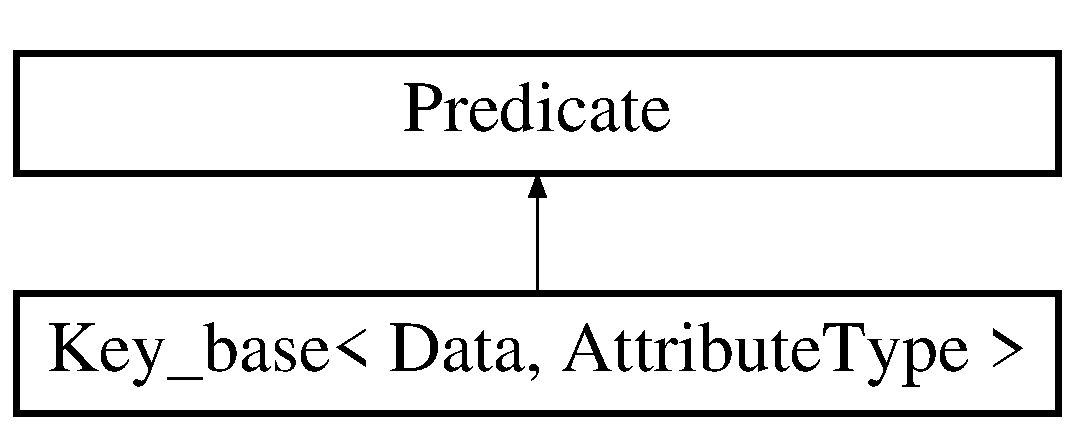
\includegraphics[height=2cm]{class_key__base}
\end{center}
\end{figure}
\subsection*{Public Member Functions}
\begin{CompactItemize}
\item 
template$<$class Input\-DBFormat$>$ {\bf Key\_\-base} (Data \&intable, Input\-DBFormat \&input)\label{class_key__base_f8742868c86280f7f169552d9e2d36fe}

\begin{CompactList}\small\item\em Constructor. \item\end{CompactList}\item 
{\bf $\sim$Key\_\-base} ()\label{class_key__base_8fd75950feb99c6c29008354d893d39c}

\begin{CompactList}\small\item\em Destructor. \item\end{CompactList}\item 
template$<$class Iterator, class Measure$>$ bool {\bf operator()} (Iterator itemset\-It, Measure \&mes\-Cand)
\begin{CompactList}\small\item\em Operator that test if a set of attributes is not redundant. \item\end{CompactList}\end{CompactItemize}
\subsection*{Protected Member Functions}
\begin{CompactItemize}
\item 
template$<$class Iterator$>$ int {\bf count\-Projection} (Iterator it\-Cand)
\begin{CompactList}\small\item\em function used to count the projection of a candidates pointed by the iterator passed in parameter. \item\end{CompactList}\end{CompactItemize}
\subsection*{Protected Attributes}
\begin{CompactItemize}
\item 
int {\bf nb\-Dist\-Tuples}\label{class_key__base_e39c979bb73d9984029b18619e7edeb1}

\begin{CompactList}\small\item\em Number of distinct tuples. \item\end{CompactList}\item 
Data $\ast$ {\bf table}\label{class_key__base_c49571273cb2ae96f540733fdfe05f4d}

\begin{CompactList}\small\item\em the tabular data \item\end{CompactList}\item 
{\bf Recode\-To\-Int}$<$ Attribute\-Type $>$ {\bf num\-Attrib}\label{class_key__base_ed8fae06f994b73f9f9f3eb1ebbac690}

\begin{CompactList}\small\item\em Used to get the numero of the attributes ( 1st, 2nd,...). \item\end{CompactList}\end{CompactItemize}
\subsection*{Classes}
\begin{CompactItemize}
\item 
class {\bf Process\-Tuples}
\begin{CompactList}\small\item\em Functor used to projet all the tuples wrt attributes studied. \item\end{CompactList}\item 
class {\bf project}
\begin{CompactList}\small\item\em Functor used to projet a tuple wrt the set of attributes studied. \item\end{CompactList}\end{CompactItemize}


\subsection{Detailed Description}
\subsubsection*{template$<$class Data, class Attribute\-Type$>$ class Key\_\-base$<$ Data, Attribute\-Type $>$}

Functor representing the predicate being not redundant. 

This functor test if an itemset is a super key. The method used to test if a candidate is a super key is the following one: the functor process the cardinality of the projection wrt the attributes of the candidate. return false if the cardinality is not equal to the number of tuples in the relation.

The template parameter Data is the type of the tablular data. The template parameter Attribute\-Type is the type of the attributes. 



\subsection{Member Function Documentation}
\index{Key_base@{Key\_\-base}!countProjection@{countProjection}}
\index{countProjection@{countProjection}!Key_base@{Key\_\-base}}
\subsubsection{\setlength{\rightskip}{0pt plus 5cm}template$<$class Data, class Attribute\-Type$>$ template$<$class Iterator$>$ int {\bf Key\_\-base}$<$ Data, Attribute\-Type $>$::count\-Projection (Iterator {\em it\-Cand})\hspace{0.3cm}{\tt  [protected]}}\label{class_key__base_2ad0e062e502dd49018ce3f60691f12d}


function used to count the projection of a candidates pointed by the iterator passed in parameter. 

\begin{Desc}
\item[Parameters:]
\begin{description}
\item[{\em it\-Cand}]iterator on the candidate to test. \end{description}
\end{Desc}
\begin{Desc}
\item[Returns:]the cardinality of the projection. \end{Desc}
\index{Key_base@{Key\_\-base}!operator()@{operator()}}
\index{operator()@{operator()}!Key_base@{Key\_\-base}}
\subsubsection{\setlength{\rightskip}{0pt plus 5cm}template$<$class Data, class Attribute\-Type$>$ template$<$class Iterator, class Measure$>$ bool {\bf Key\_\-base}$<$ Data, Attribute\-Type $>$::operator() (Iterator {\em it\-Cand}, Measure \& {\em mes\-Cand})}\label{class_key__base_27f6933ca653e959cea1332231c1ee8a}


Operator that test if a set of attributes is not redundant. 

\begin{Desc}
\item[Parameters:]
\begin{description}
\item[{\em it\-Cand}]iterator (or pointer) on the set of attributes to test wrt the predicate \item[{\em mes\-Cand}]cardinality of the projection on the db of the attributes \end{description}
\end{Desc}


Reimplemented from {\bf Predicate} {\rm (p.\,\pageref{class_predicate_6fb1a75dba2268f75738f335f403e46c})}.

The documentation for this class was generated from the following file:\begin{CompactItemize}
\item 
F:/i\-Zi/problems/key/Key\_\-base.hxx\end{CompactItemize}

\section{Key\_\-base$<$ Data, Attribute\-Type $>$::Process\-Tuples$<$ Iterator $>$ Class Template Reference}
\label{class_key__base_1_1_process_tuples}\index{Key_base::ProcessTuples@{Key\_\-base::ProcessTuples}}
Functor used to projet all the tuples wrt attributes studied.  


{\tt \#include $<$Key\_\-base.hxx$>$}



\subsection{Detailed Description}
\subsubsection*{template$<$class Data, class Attribute\-Type$>$template$<$class Iterator$>$ class Key\_\-base$<$ Data, Attribute\-Type $>$::Process\-Tuples$<$ Iterator $>$}

Functor used to projet all the tuples wrt attributes studied. 



The documentation for this class was generated from the following file:\begin{CompactItemize}
\item 
F:/i\-Zi/problems/key/Key\_\-base.hxx\end{CompactItemize}

\section{Key\_\-base$<$ Data, Attribute\-Type $>$::project$<$ Container\-Tuple $>$ Class Template Reference}
\label{class_key__base_1_1project}\index{Key_base::project@{Key\_\-base::project}}
Functor used to projet a tuple wrt the set of attributes studied.  


{\tt \#include $<$Key\_\-base.hxx$>$}



\subsection{Detailed Description}
\subsubsection*{template$<$class Data, class Attribute\-Type$>$template$<$class Container\-Tuple$>$ class Key\_\-base$<$ Data, Attribute\-Type $>$::project$<$ Container\-Tuple $>$}

Functor used to projet a tuple wrt the set of attributes studied. 



The documentation for this class was generated from the following file:\begin{CompactItemize}
\item 
F:/i\-Zi/problems/key/Key\_\-base.hxx\end{CompactItemize}

\section{Node$<$ Sets\-Type, Measure $>$ Class Template Reference}
\label{class_node}\index{Node@{Node}}
Class representing a node of the {\bf PTree}{\rm (p.\,\pageref{class_p_tree})}.  


{\tt \#include $<$Node.hxx$>$}

\subsection*{Public Member Functions}
\begin{CompactItemize}
\item 
template$<$class Container$>$ int {\bf push\_\-back} (Container \&set\-Element, Measure nb=Measure())
\begin{CompactList}\small\item\em Push back a set of element in the trie. \item\end{CompactList}\item 
template$<$class Input\-Iterator$>$ int {\bf push\_\-back} (Input\-Iterator \&first, Input\-Iterator \&last, Measure nb=Measure())
\begin{CompactList}\small\item\em Push back a set of element in the trie. \item\end{CompactList}\item 
template$<$class Container$>$ int {\bf insert\-Child\-Node} (int intid, Container \&set\-Element, Measure nb=Measure())
\begin{CompactList}\small\item\em Insert in child nodes to the current one. \item\end{CompactList}\item 
template$<$class Input\-Iterator$>$ int {\bf insert\-Child\-Node} (int intid, Input\-Iterator \&first, Input\-Iterator \&last, Measure nb=Measure())
\begin{CompactList}\small\item\em Insert in child nodes to the current one. \item\end{CompactList}\item 
int {\bf delete\-It\-Vect} (int index)
\item 
void {\bf add\-It\-Vect} (int item, {\bf Node} $\ast$ins\-Child=0, int sizecnts=1, int sizechilds=1)
\item 
{\bf Node} (const {\bf Node} \&in\-Node)
\item 
int {\bf delete\-Children} ()
\item 
{\bf Node} $\ast$ {\bf insert} (int $\ast$itemset, int level, Measure in\-Sup=Measure(true))
\item 
bool {\bf delete\-It} (vect\-UI $\ast$itemset, int \&pos)
\item 
void {\bf print} ({\bf Recode\-To\-Int}$<$ Sets\-Type $>$ $\ast$recode=0)
\item 
int {\bf read\-Itemsets} (const char $\ast$file\-Name, int $\ast$remap=0)
\item 
void {\bf save\-Itemsets} (const char $\ast$file\-Name, int $\ast$remap=0)
\item 
void {\bf save} (const char $\ast$file\-Name, {\bf Recode\-To\-Int}$<$ Sets\-Type $>$ $\ast$recode=0)
\item 
void {\bf save\-Data\-Set} (const char $\ast$file\-Name, int $\ast$remap=0)
\item 
bool {\bf included\-In} (int $\ast$itemset, int level, int spos=0)
\item 
bool {\bf include} (vect\-UI $\ast$itemset, int spos=0)
\item 
{\bf Node} $\ast$ {\bf complem} (vect\-UI \&list\-Elem, int \&max\-Size)
\item 
int {\bf gen\-Subsets} (vect\-UI $\ast$itemset, int spos, int depth)
\item 
{\bf Node} $\ast$ {\bf gen\-Subsets} (int size)
\end{CompactItemize}
\subsection*{Protected Attributes}
\begin{CompactItemize}
\item 
{\bf Node} $\ast$ {\bf parent}\label{class_node_039a14ac4e2dd6be991d7d81cf902296}

\begin{CompactList}\small\item\em Parent node. \item\end{CompactList}\item 
int {\bf id}\label{class_node_2a5bd864397d5f9015772e9163846f0f}

\begin{CompactList}\small\item\em Item (internal id) in the parent node. \item\end{CompactList}\item 
int {\bf offset}\label{class_node_23587c472f965fdb345553da8c43efbd}

\begin{CompactList}\small\item\em Offset of counter vector. \item\end{CompactList}\item 
vect\-T $\ast$ {\bf cnts}\label{class_node_9b5fd38081c3726f4b0080013dec36b1}

\begin{CompactList}\small\item\em \char`\"{}bool vector\char`\"{} used to represents the presence or not of an element. \item\end{CompactList}\item 
vect\-N $\ast$ {\bf childs}\label{class_node_ead9baf380a8c18deaf8cf3f4469c849}

\begin{CompactList}\small\item\em Pointer on the corresponding child nodes. \item\end{CompactList}\end{CompactItemize}
\subsection*{Friends}
\begin{CompactItemize}
\item 
class {\bf It\-PTree$<$ Sets\-Type, Measure $>$}\label{class_node_c7d742f89a5418f941e82b344fe4c463}

\item 
class {\bf PTree$<$ Sets\-Type, Measure $>$}\label{class_node_75985e4c63d08b10230ccb3b9f097182}

\end{CompactItemize}


\subsection{Detailed Description}
\subsubsection*{template$<$class Sets\-Type, class Measure = Boolean$>$ class Node$<$ Sets\-Type, Measure $>$}

Class representing a node of the {\bf PTree}{\rm (p.\,\pageref{class_p_tree})}. 

The template parameter Measure represents the type of the \char`\"{}bool vector\char`\"{} used to represents the presence or not of an element. For example bool to only store the presence or not of the element, int to store an integer measure (such as the support)...

The template parameter Sets\-Type represents the type of the elements inserted in the trie. The template parameter Measure is eventually used to store additional informations associted with the sets stored. 



\subsection{Constructor \& Destructor Documentation}
\index{Node@{Node}!Node@{Node}}
\index{Node@{Node}!Node@{Node}}
\subsubsection{\setlength{\rightskip}{0pt plus 5cm}template$<$class Sets\-Type, class Measure$>$ {\bf Node}$<$ Sets\-Type, Measure $>$::{\bf Node} (const {\bf Node}$<$ Sets\-Type, Measure $>$ \& {\em in\-Node})}\label{class_node_796ed77ffb6aa900993ce9b4a9700c1d}


Recopy Constructor 

\subsection{Member Function Documentation}
\index{Node@{Node}!addItVect@{addItVect}}
\index{addItVect@{addItVect}!Node@{Node}}
\subsubsection{\setlength{\rightskip}{0pt plus 5cm}template$<$class Sets\-Type, class Measure$>$ void {\bf Node}$<$ Sets\-Type, Measure $>$::add\-It\-Vect (int {\em item}, {\bf Node}$<$ Sets\-Type, Measure $>$ $\ast$ {\em ins\-Child} = {\tt 0}, int {\em sizecnts} = {\tt 1}, int {\em sizechilds} = {\tt 1})}\label{class_node_e5ee3b6e405b43d3358288f5c8e521c1}


method that allocate new memory in the counters vector and modify the childs vector if necessary item is the new item to insert in the cnts vector ins\-Child is not null if we want to insert ins\-Child as a child of the new item being inserted sizecnts and sizechilds are the min size of vectors allocated at creation \index{Node@{Node}!complem@{complem}}
\index{complem@{complem}!Node@{Node}}
\subsubsection{\setlength{\rightskip}{0pt plus 5cm}template$<$class Sets\-Type, class Measure$>$ {\bf Node}$<$ Sets\-Type, Measure $>$ $\ast$ {\bf Node}$<$ Sets\-Type, Measure $>$::complem (vect\-UI \& {\em list\-Elem}, int \& {\em max\-Size})}\label{class_node_a3be41dd7d34b71421bcce51edfd1516}


method that return the complementary of this set of itemset (res) since we have all the items ordered and with the internal id begining at 1 to the number of items in the database we only have to use the total number of items to find the complementary \index{Node@{Node}!deleteChildren@{deleteChildren}}
\index{deleteChildren@{deleteChildren}!Node@{Node}}
\subsubsection{\setlength{\rightskip}{0pt plus 5cm}template$<$class Sets\-Type, class Measure$>$ int {\bf Node}$<$ Sets\-Type, Measure $>$::delete\-Children ()}\label{class_node_51768328ab596c30ad943eb132b77d67}


method that delete recursively the sub {\bf Node}{\rm (p.\,\pageref{class_node})} of this node \index{Node@{Node}!deleteIt@{deleteIt}}
\index{deleteIt@{deleteIt}!Node@{Node}}
\subsubsection{\setlength{\rightskip}{0pt plus 5cm}template$<$class Sets\-Type, class Measure$>$ bool {\bf Node}$<$ Sets\-Type, Measure $>$::delete\-It (vect\-UI $\ast$ {\em itemset}, int \& {\em pos})}\label{class_node_98000cdef313e203299526f92d3215c9}


method which delete an itemset in a set of itemset \index{Node@{Node}!deleteItVect@{deleteItVect}}
\index{deleteItVect@{deleteItVect}!Node@{Node}}
\subsubsection{\setlength{\rightskip}{0pt plus 5cm}template$<$class Sets\-Type, class Measure$>$ int {\bf Node}$<$ Sets\-Type, Measure $>$::delete\-It\-Vect (int {\em index})}\label{class_node_8be4d0c5c3d8c8aa8e91c1f2aac0b119}


method that delete the index-th item of the counters vector, and modify the childs vector if necessary ( the memory allocated to the vectors is reallocated wrt the modifications) return the current value of index (result +1 will be the new current value ) \index{Node@{Node}!genSubsets@{genSubsets}}
\index{genSubsets@{genSubsets}!Node@{Node}}
\subsubsection{\setlength{\rightskip}{0pt plus 5cm}template$<$class Sets\-Type, class Measure$>$ {\bf Node}$<$ Sets\-Type, Measure $>$ $\ast$ {\bf Node}$<$ Sets\-Type, Measure $>$::gen\-Subsets (int {\em size})}\label{class_node_ddd4e181cfc9990fff6e966a076cf0de}


method that return a set of the subsets of size \char`\"{}size\char`\"{} of this set of itemsets \index{Node@{Node}!genSubsets@{genSubsets}}
\index{genSubsets@{genSubsets}!Node@{Node}}
\subsubsection{\setlength{\rightskip}{0pt plus 5cm}template$<$class Sets\-Type, class Measure$>$ int {\bf Node}$<$ Sets\-Type, Measure $>$::gen\-Subsets (vect\-UI $\ast$ {\em itemset}, int {\em spos}, int {\em depth})}\label{class_node_767d9fa45fed21095d870913db775be6}


method that generate into this set the subsets of size \char`\"{}size\char`\"{} of an itemsets of size k \index{Node@{Node}!include@{include}}
\index{include@{include}!Node@{Node}}
\subsubsection{\setlength{\rightskip}{0pt plus 5cm}template$<$class Sets\-Type, class Measure$>$ bool {\bf Node}$<$ Sets\-Type, Measure $>$::include (vect\-UI $\ast$ {\em itemset}, int {\em spos} = {\tt 0})}\label{class_node_7d48901c2a01e373b4273bf92b2edf58}


method searching if itemset is include in one of the itemsets of this set of itemset \index{Node@{Node}!includedIn@{includedIn}}
\index{includedIn@{includedIn}!Node@{Node}}
\subsubsection{\setlength{\rightskip}{0pt plus 5cm}template$<$class Sets\-Type, class Measure$>$ bool {\bf Node}$<$ Sets\-Type, Measure $>$::included\-In (int $\ast$ {\em itemset}, int {\em level}, int {\em spos} = {\tt 0})}\label{class_node_50472949d567c7a05548943eb8ce11d6}


method searching if one itemset of of the sub tree rooted by this node is included into \char`\"{}itemset\char`\"{} be carefull itemset MUST BE ordered \index{Node@{Node}!insert@{insert}}
\index{insert@{insert}!Node@{Node}}
\subsubsection{\setlength{\rightskip}{0pt plus 5cm}template$<$class Sets\-Type, class Measure$>$ {\bf Node}$<$ Sets\-Type, Measure $>$ $\ast$ {\bf Node}$<$ Sets\-Type, Measure $>$::insert (int $\ast$ {\em itemset}, int {\em level}, Measure {\em in\-Sup} = {\tt Measure(true)})}\label{class_node_7fade38fb4e2f586dd2287bcbfb9a6c8}


method which insert an itemset in the sub tree rooted by the current node size\-Alloc determine the size allocated (reserved) to the childs at initilisation vector. If = to 0 the allocation is dynamically made when a new inserted item imply to enlarge the vector ( new memory allocation and recopy of the olds Vals are made) \index{Node@{Node}!insertChildNode@{insertChildNode}}
\index{insertChildNode@{insertChildNode}!Node@{Node}}
\subsubsection{\setlength{\rightskip}{0pt plus 5cm}template$<$class Sets\-Type, class Measure = Boolean$>$ template$<$class Input\-Iterator$>$ int {\bf Node}$<$ Sets\-Type, Measure $>$::insert\-Child\-Node (int {\em intid}, Input\-Iterator \& {\em first}, Input\-Iterator \& {\em last}, Measure {\em nb} = {\tt Measure()})\hspace{0.3cm}{\tt  [inline]}}\label{class_node_6b56a65665f8100dc369fdda64691ee3}


Insert in child nodes to the current one. 

\begin{Desc}
\item[Parameters:]
\begin{description}
\item[{\em intid}]internal id of the current element in the node \item[{\em first}]iterator on the first element \item[{\em last}]iterator on the element after the last \item[{\em nb}]the number of times the set is inserted \end{description}
\end{Desc}
\begin{Desc}
\item[Returns:]the size of the set inserted (if 0 the set was already in the trie) \end{Desc}
\index{Node@{Node}!insertChildNode@{insertChildNode}}
\index{insertChildNode@{insertChildNode}!Node@{Node}}
\subsubsection{\setlength{\rightskip}{0pt plus 5cm}template$<$class Sets\-Type, class Measure = Boolean$>$ template$<$class Container$>$ int {\bf Node}$<$ Sets\-Type, Measure $>$::insert\-Child\-Node (int {\em intid}, Container \& {\em set\-Element}, Measure {\em nb} = {\tt Measure()})\hspace{0.3cm}{\tt  [inline]}}\label{class_node_d1a110523a143505c594b0be9ae65626}


Insert in child nodes to the current one. 

\begin{Desc}
\item[Parameters:]
\begin{description}
\item[{\em intid}]internal id of the current element in the node \item[{\em set\-Element}]the set of element to insert in the trie \item[{\em nb}]the number of times the set is inserted \end{description}
\end{Desc}
\begin{Desc}
\item[Returns:]the size of the set inserted (if 0 the set was already in the trie) \end{Desc}
\index{Node@{Node}!print@{print}}
\index{print@{print}!Node@{Node}}
\subsubsection{\setlength{\rightskip}{0pt plus 5cm}template$<$class Sets\-Type, class Measure$>$ void {\bf Node}$<$ Sets\-Type, Measure $>$::print ({\bf Recode\-To\-Int}$<$ Sets\-Type $>$ $\ast$ {\em recode} = {\tt 0})}\label{class_node_f4040669d0f5f254a01a07b631fceec0}


print to screen all the itemset stored in the sub tree remap is a table for mapping the name of the items \index{Node@{Node}!push_back@{push\_\-back}}
\index{push_back@{push\_\-back}!Node@{Node}}
\subsubsection{\setlength{\rightskip}{0pt plus 5cm}template$<$class Sets\-Type, class Measure = Boolean$>$ template$<$class Input\-Iterator$>$ int {\bf Node}$<$ Sets\-Type, Measure $>$::push\_\-back (Input\-Iterator \& {\em first}, Input\-Iterator \& {\em last}, Measure {\em nb} = {\tt Measure()})\hspace{0.3cm}{\tt  [inline]}}\label{class_node_6fd6696c9ee3f0b189b0d8f00ff53b34}


Push back a set of element in the trie. 

The template parameter represents the input iterators on the integers to insert int the trie. \begin{Desc}
\item[Parameters:]
\begin{description}
\item[{\em first}]iterator on the first element \item[{\em last}]iterator on the element after the last \item[{\em nb}]the number of times the set is inserted \end{description}
\end{Desc}
\begin{Desc}
\item[Returns:]the size of the set inserted (if 0 the set was already in the trie) \end{Desc}
\index{Node@{Node}!push_back@{push\_\-back}}
\index{push_back@{push\_\-back}!Node@{Node}}
\subsubsection{\setlength{\rightskip}{0pt plus 5cm}template$<$class Sets\-Type, class Measure = Boolean$>$ template$<$class Container$>$ int {\bf Node}$<$ Sets\-Type, Measure $>$::push\_\-back (Container \& {\em set\-Element}, Measure {\em nb} = {\tt Measure()})\hspace{0.3cm}{\tt  [inline]}}\label{class_node_cca2b11c6bdb5944d3dbe558383113f5}


Push back a set of element in the trie. 

This function corresponds to the classic {\bf push\_\-back( )}{\rm (p.\,\pageref{class_node_cca2b11c6bdb5944d3dbe558383113f5})} function od STL container. The template parameter represents a container of integers. \begin{Desc}
\item[Parameters:]
\begin{description}
\item[{\em set\-Element}]the set of element to insert in the trie \item[{\em nb}]the number of times the set is inserted \end{description}
\end{Desc}
\begin{Desc}
\item[Returns:]the size of the set inserted (if 0 the set was already in the trie) \end{Desc}
\index{Node@{Node}!readItemsets@{readItemsets}}
\index{readItemsets@{readItemsets}!Node@{Node}}
\subsubsection{\setlength{\rightskip}{0pt plus 5cm}template$<$class Sets\-Type, class Measure$>$ int {\bf Node}$<$ Sets\-Type, Measure $>$::read\-Itemsets (const char $\ast$ {\em file\-Name}, int $\ast$ {\em remap} = {\tt 0})}\label{class_node_05afc346678e3d677af92ae0941ace66}


read from a file all the itemset and stored them into a prefix tree \index{Node@{Node}!save@{save}}
\index{save@{save}!Node@{Node}}
\subsubsection{\setlength{\rightskip}{0pt plus 5cm}template$<$class Sets\-Type, class Measure$>$ void {\bf Node}$<$ Sets\-Type, Measure $>$::save (const char $\ast$ {\em file\-Name}, {\bf Recode\-To\-Int}$<$ Sets\-Type $>$ $\ast$ {\em recode} = {\tt 0})}\label{class_node_bab17c04ff98392f552c2e0fb21ae8b2}


save into a file all the itemset stored in tree remap is a table for mapping the name of the items if remap is 0 it use the internal id \index{Node@{Node}!saveDataSet@{saveDataSet}}
\index{saveDataSet@{saveDataSet}!Node@{Node}}
\subsubsection{\setlength{\rightskip}{0pt plus 5cm}template$<$class Sets\-Type, class Measure$>$ void {\bf Node}$<$ Sets\-Type, Measure $>$::save\-Data\-Set (const char $\ast$ {\em file\-Name}, int $\ast$ {\em remap} = {\tt 0})}\label{class_node_e57e552e42262a283c14f8f522b1ba16}


save into a file all the itemset stored in tree remap is a table for mapping the name of the items according the FIMI format of datasets \index{Node@{Node}!saveItemsets@{saveItemsets}}
\index{saveItemsets@{saveItemsets}!Node@{Node}}
\subsubsection{\setlength{\rightskip}{0pt plus 5cm}template$<$class Sets\-Type, class Measure$>$ void {\bf Node}$<$ Sets\-Type, Measure $>$::save\-Itemsets (const char $\ast$ {\em file\-Name}, int $\ast$ {\em remap} = {\tt 0})}\label{class_node_80f20886fd8cfda7e36a2ee0ba761c2c}


save into a file all the itemset stored in tree remap is a table for mapping the name of the items if remap is 0 it use the internal id 

The documentation for this class was generated from the following file:\begin{CompactItemize}
\item 
F:/i\-Zi/data\-Structures/trie/Node.hxx\end{CompactItemize}

\section{No\-Output Class Reference}
\label{class_no_output}\index{NoOutput@{NoOutput}}
class used to not store/output a solution of the algorithm.  


{\tt \#include $<$No\-Output.hxx$>$}



\subsection{Detailed Description}
class used to not store/output a solution of the algorithm. 

Using this class and the variable none the user select no output for a solution of the algorithm. For example if the theory parameter is set to \char`\"{}none\char`\"{} the algorithm will not store the theory. 



The documentation for this class was generated from the following file:\begin{CompactItemize}
\item 
F:/i\-Zi/util/No\-Output.hxx\end{CompactItemize}

\section{Not\_\-Predicate$<$ Predicate\-Neg $>$ Class Template Reference}
\label{class_not___predicate}\index{Not_Predicate@{Not\_\-Predicate}}
{\bf Predicate}{\rm (p.\,\pageref{class_predicate})} that return the negation of a predicate passed in parameter.  


{\tt \#include $<$Not\_\-Predicate.hxx$>$}

Inheritance diagram for Not\_\-Predicate$<$ Predicate\-Neg $>$::\begin{figure}[H]
\begin{center}
\leavevmode
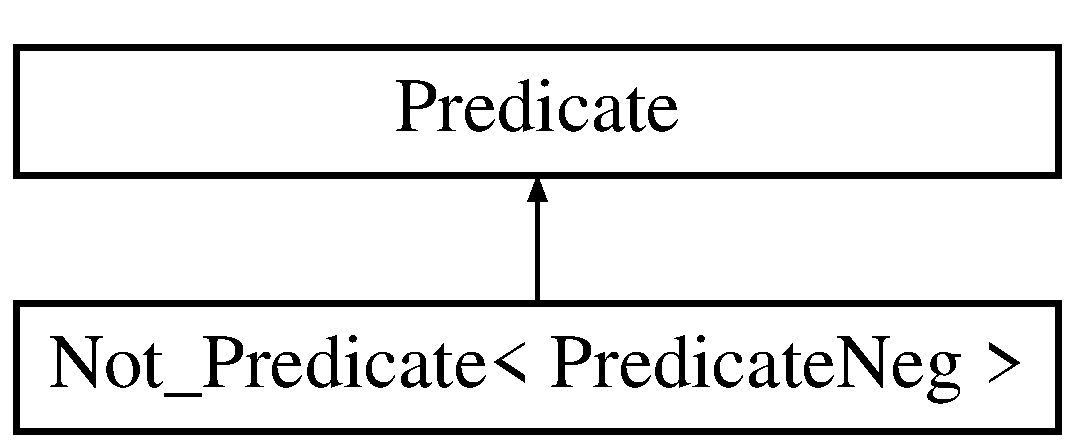
\includegraphics[height=2cm]{class_not___predicate}
\end{center}
\end{figure}
\subsection*{Public Member Functions}
\begin{CompactItemize}
\item 
{\bf Not\_\-Predicate} (Predicate\-Neg \&in\-Pred)\label{class_not___predicate_48a08a2ead6b824a9fec80c3610ccba7}

\begin{CompactList}\small\item\em Constructor. \item\end{CompactList}\item 
template$<$class Iterator, class Measure$>$ bool {\bf operator()} (Iterator it\-Cand, Measure \&mes\-Cand)\label{class_not___predicate_c4dd938a356c8476e50806158069d169}

\begin{CompactList}\small\item\em Operator that test if a set of attributes is not redundant. \item\end{CompactList}\item 
template$<$class Cand\_\-Data\-Struct, class f$>$ void {\bf pre\-Processing} (Cand\_\-Data\-Struct \&cand, f \&word\-To\-Set)
\begin{CompactList}\small\item\em Function used to do some pre processing operations before testing the candidates generated. \item\end{CompactList}\item 
template$<$class Cand\_\-Data\-Struct, class f$>$ void {\bf post\-Processing} (Cand\_\-Data\-Struct \&cand, f \&word\-To\-Set)
\begin{CompactList}\small\item\em Function used to do some post processing operations after testing the candidates generated. \item\end{CompactList}\end{CompactItemize}
\subsection*{Protected Attributes}
\begin{CompactItemize}
\item 
Predicate\-Neg $\ast$ {\bf pred}\label{class_not___predicate_2dff4f17e32eeae61ee949f76e542ff5}

\begin{CompactList}\small\item\em {\bf Predicate}{\rm (p.\,\pageref{class_predicate})} to studied. \item\end{CompactList}\end{CompactItemize}


\subsection{Detailed Description}
\subsubsection*{template$<$class Predicate\-Neg$>$ class Not\_\-Predicate$<$ Predicate\-Neg $>$}

{\bf Predicate}{\rm (p.\,\pageref{class_predicate})} that return the negation of a predicate passed in parameter. 



\subsection{Member Function Documentation}
\index{Not_Predicate@{Not\_\-Predicate}!postProcessing@{postProcessing}}
\index{postProcessing@{postProcessing}!Not_Predicate@{Not\_\-Predicate}}
\subsubsection{\setlength{\rightskip}{0pt plus 5cm}template$<$class Predicate\-Neg$>$ template$<$class Cand\_\-Data\-Struct, class f$>$ void {\bf Not\_\-Predicate}$<$ Predicate\-Neg $>$::post\-Processing (Cand\_\-Data\-Struct \& {\em cand}, f \& {\em word\-To\-Set})\hspace{0.3cm}{\tt  [inline]}}\label{class_not___predicate_849572f82b1b8a34b9b71459c9da24be}


Function used to do some post processing operations after testing the candidates generated. 

\begin{Desc}
\item[Parameters:]
\begin{description}
\item[{\em cand}]container of words of the language. \end{description}
\end{Desc}
\index{Not_Predicate@{Not\_\-Predicate}!preProcessing@{preProcessing}}
\index{preProcessing@{preProcessing}!Not_Predicate@{Not\_\-Predicate}}
\subsubsection{\setlength{\rightskip}{0pt plus 5cm}template$<$class Predicate\-Neg$>$ template$<$class Cand\_\-Data\-Struct, class f$>$ void {\bf Not\_\-Predicate}$<$ Predicate\-Neg $>$::pre\-Processing (Cand\_\-Data\-Struct \& {\em cand}, f \& {\em word\-To\-Set})\hspace{0.3cm}{\tt  [inline]}}\label{class_not___predicate_8282dfa9cdd77232c633264d73cab680}


Function used to do some pre processing operations before testing the candidates generated. 

\begin{Desc}
\item[Parameters:]
\begin{description}
\item[{\em cand}]container of words of the language. \end{description}
\end{Desc}


The documentation for this class was generated from the following file:\begin{CompactItemize}
\item 
F:/i\-Zi/algorithms/Not\_\-Predicate.hxx\end{CompactItemize}

\section{Predicate Class Reference}
\label{class_predicate}\index{Predicate@{Predicate}}
Mother abstract functor representing a predicate.  


{\tt \#include $<$Predicate.hxx$>$}

Inheritance diagram for Predicate::\begin{figure}[H]
\begin{center}
\leavevmode
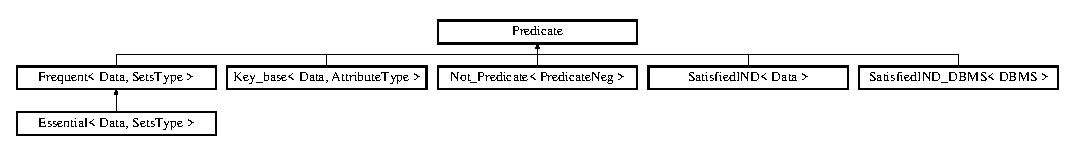
\includegraphics[height=1.6cm]{class_predicate}
\end{center}
\end{figure}
\subsection*{Public Member Functions}
\begin{CompactItemize}
\item 
{\bf Predicate} ()\label{class_predicate_50088fcbd7632e6be3b2df62441535af}

\begin{CompactList}\small\item\em Constructor. \item\end{CompactList}\item 
virtual {\bf $\sim$Predicate} ()\label{class_predicate_91060d92c2f251fd3b0072a3c08f3911}

\begin{CompactList}\small\item\em Destructor. \item\end{CompactList}\item 
template$<$class Iterator, class Measure$>$ bool {\bf operator()} (Iterator word\-It, Measure \&mes\-Cand)
\begin{CompactList}\small\item\em Operator that test if a word of the language is interesting wrt predicate or not. \item\end{CompactList}\item 
template$<$class Cand\_\-Data\-Struct, class f$>$ void {\bf pre\-Processing} (Cand\_\-Data\-Struct \&cand, f word\-To\-Set)
\begin{CompactList}\small\item\em Function used to do some pre processing operations before testing the candidates generated. \item\end{CompactList}\item 
template$<$class Cand\_\-Data\-Struct, class f$>$ void {\bf post\-Processing} (Cand\_\-Data\-Struct \&cand, f word\-To\-Set)
\begin{CompactList}\small\item\em Function used to do some post processing operations after testing the candidates generated. \item\end{CompactList}\end{CompactItemize}


\subsection{Detailed Description}
Mother abstract functor representing a predicate. 

This functor test if an itemset is interesting wrt the predicate. The template parameter Iterator is an iterator on a candidate. 



\subsection{Member Function Documentation}
\index{Predicate@{Predicate}!operator()@{operator()}}
\index{operator()@{operator()}!Predicate@{Predicate}}
\subsubsection{\setlength{\rightskip}{0pt plus 5cm}template$<$class Iterator, class Measure$>$ bool Predicate::operator() (Iterator {\em word\-It}, Measure \& {\em mes\-Cand})\hspace{0.3cm}{\tt  [inline]}}\label{class_predicate_6fb1a75dba2268f75738f335f403e46c}


Operator that test if a word of the language is interesting wrt predicate or not. 

\begin{Desc}
\item[Parameters:]
\begin{description}
\item[{\em word\-It}]iterator on the word to test. \end{description}
\end{Desc}


Reimplemented in {\bf Not\_\-Predicate$<$ Predicate\-Neg $>$} {\rm (p.\,\pageref{class_not___predicate_c4dd938a356c8476e50806158069d169})}, {\bf Satisfied\-IND$<$ Data $>$} {\rm (p.\,\pageref{class_satisfied_i_n_d_bbf69fd5dfbf71f8e7f0685b80551c6d})}, {\bf Satisfied\-IND\_\-DBMS$<$ DBMS $>$} {\rm (p.\,\pageref{class_satisfied_i_n_d___d_b_m_s_10cb098e49804f3de10b20c1d3317814})}, {\bf Essential$<$ Data, Sets\-Type $>$} {\rm (p.\,\pageref{class_essential_e6a89fa2543fe441619066b0f4f6323b})}, {\bf Frequent$<$ Data, Sets\-Type $>$} {\rm (p.\,\pageref{class_frequent_82e02ab1cf1749ea52e9603dc06a5d15})}, and {\bf Key\_\-base$<$ Data, Attribute\-Type $>$} {\rm (p.\,\pageref{class_key__base_27f6933ca653e959cea1332231c1ee8a})}.\index{Predicate@{Predicate}!postProcessing@{postProcessing}}
\index{postProcessing@{postProcessing}!Predicate@{Predicate}}
\subsubsection{\setlength{\rightskip}{0pt plus 5cm}template$<$class Cand\_\-Data\-Struct, class f$>$ void Predicate::post\-Processing (Cand\_\-Data\-Struct \& {\em cand}, f {\em word\-To\-Set})\hspace{0.3cm}{\tt  [inline]}}\label{class_predicate_49f7acb334fac851a26a4d1aecc64571}


Function used to do some post processing operations after testing the candidates generated. 

\begin{Desc}
\item[Parameters:]
\begin{description}
\item[{\em cand}]container of words of the language. \end{description}
\end{Desc}


Reimplemented in {\bf Frequent$<$ Data, Sets\-Type $>$} {\rm (p.\,\pageref{class_frequent_ff29167beb828195c34e10881abb2f74})}.\index{Predicate@{Predicate}!preProcessing@{preProcessing}}
\index{preProcessing@{preProcessing}!Predicate@{Predicate}}
\subsubsection{\setlength{\rightskip}{0pt plus 5cm}template$<$class Cand\_\-Data\-Struct, class f$>$ void Predicate::pre\-Processing (Cand\_\-Data\-Struct \& {\em cand}, f {\em word\-To\-Set})\hspace{0.3cm}{\tt  [inline]}}\label{class_predicate_8ee59d790e9b46e5e0555dbeb5b91f95}


Function used to do some pre processing operations before testing the candidates generated. 

\begin{Desc}
\item[Parameters:]
\begin{description}
\item[{\em cand}]container of words of the language. \end{description}
\end{Desc}


Reimplemented in {\bf Frequent$<$ Data, Sets\-Type $>$} {\rm (p.\,\pageref{class_frequent_236bb06ebfac503436c8a25a8507b467})}.

The documentation for this class was generated from the following file:\begin{CompactItemize}
\item 
F:/i\-Zi/problems/Predicate.hxx\end{CompactItemize}

\section{print\-Container Class Reference}
\label{classprint_container}\index{printContainer@{printContainer}}
Functor used to print to screen a container.  


{\tt \#include $<$Recode\-To\-Int.hxx$>$}



\subsection{Detailed Description}
Functor used to print to screen a container. 



The documentation for this class was generated from the following file:\begin{CompactItemize}
\item 
F:/i\-Zi/util/Recode\-To\-Int.hxx\end{CompactItemize}

\section{print\-Container\-Of\-Container Class Reference}
\label{classprint_container_of_container}\index{printContainerOfContainer@{printContainerOfContainer}}
Functor used to print to screen a container of container.  


{\tt \#include $<$Recode\-To\-Int.hxx$>$}



\subsection{Detailed Description}
Functor used to print to screen a container of container. 



The documentation for this class was generated from the following file:\begin{CompactItemize}
\item 
F:/i\-Zi/util/Recode\-To\-Int.hxx\end{CompactItemize}

\section{print\-Container\-Of\-Iterator$<$ Type $>$ Class Template Reference}
\label{classprint_container_of_iterator}\index{printContainerOfIterator@{printContainerOfIterator}}
Functor used to print to screen a container of iterator on elements.  


{\tt \#include $<$Recode\-To\-Int.hxx$>$}



\subsection{Detailed Description}
\subsubsection*{template$<$class Type$>$ class print\-Container\-Of\-Iterator$<$ Type $>$}

Functor used to print to screen a container of iterator on elements. 



The documentation for this class was generated from the following file:\begin{CompactItemize}
\item 
F:/i\-Zi/util/Recode\-To\-Int.hxx\end{CompactItemize}

\section{PTree$<$ Sets\-Type, T $>$ Class Template Reference}
\label{class_p_tree}\index{PTree@{PTree}}
Template class representing a trie data structure of integer.  


{\tt \#include $<$PTree.hxx$>$}

\subsection*{Public Types}
\begin{CompactItemize}
\item 
typedef {\bf It\-PTree}$<$ Sets\-Type, T $>$ {\bf iterator}\label{class_p_tree_aa29b0935d154c06ff0dfcacbff2d683}

\begin{CompactList}\small\item\em Used to have the same syntax tha the STL. \item\end{CompactList}\end{CompactItemize}
\subsection*{Public Member Functions}
\begin{CompactItemize}
\item 
{\bf PTree} ({\bf Node}$<$ Sets\-Type, T $>$ $\ast$in\-Head=0, int in\-Size=0, int in\-Height=0)\label{class_p_tree_36e06775df6b20cad49bc53612744f33}

\begin{CompactList}\small\item\em Constructor. \item\end{CompactList}\item 
{\bf PTree} (const {\bf PTree} \&t)\label{class_p_tree_baf9201e7e17e366e1daaf82e4c059c5}

\begin{CompactList}\small\item\em Copy constructor. \item\end{CompactList}\item 
{\bf $\sim$PTree} ()\label{class_p_tree_8d8d9d39e2e7cea5c88c56a6e2d99f83}

\begin{CompactList}\small\item\em Destructor. \item\end{CompactList}\item 
template$<$class Container$>$ void {\bf push\_\-back} (Container \&set\-Element, T nb=T(1))
\begin{CompactList}\small\item\em Insert a set of element in the trie. \item\end{CompactList}\item 
template$<$class Input\-Iterator$>$ void {\bf push\_\-back} (Input\-Iterator first, Input\-Iterator last, T nb=T(1))
\begin{CompactList}\small\item\em Insert a set of element in the trie. \item\end{CompactList}\item 
void {\bf erase} ({\bf iterator} \&position)
\begin{CompactList}\small\item\em Erase a set in the trie. \item\end{CompactList}\item 
template$<$class Container$>$ void {\bf add\-To\-Node} ({\bf iterator} \&position, Container \&set\-Element, T nb=T(1))
\begin{CompactList}\small\item\em Insert a set of element to the node pointed by an iterator. \item\end{CompactList}\item 
template$<$class Input\-Iterator$>$ void {\bf add\-To\-Node} ({\bf iterator} \&position, Input\-Iterator first, Input\-Iterator last, T nb=T(1))
\begin{CompactList}\small\item\em Insert a set of element to the node pointed by an iterator. \item\end{CompactList}\item 
{\bf iterator} {\bf erase\-Node} ({\bf iterator} \&it)
\begin{CompactList}\small\item\em Erase the node under the iterator. \item\end{CompactList}\item 
{\bf It\-PTree}$<$ Sets\-Type, T $>$ {\bf begin\-Leaf} ()\label{class_p_tree_9be852a43758de579be2642e5dc82334}

\begin{CompactList}\small\item\em Return an iterator on the first leaf of the trie (exploring the trie from the left to the right). \item\end{CompactList}\item 
{\bf It\-PTree}$<$ Sets\-Type, T $>$ {\bf rbegin\-Leaf} ()\label{class_p_tree_61ab00242ada00f83f6210efa337e065}

\begin{CompactList}\small\item\em Return an iterator on the first leaf of the trie (exploring the trie from the right to the left). \item\end{CompactList}\item 
{\bf It\-PTree}$<$ Sets\-Type, T $>$ {\bf begin\-Root} ()\label{class_p_tree_7a13989068c070cd0c63517859aff760}

\begin{CompactList}\small\item\em Return an iterator on the root node of the trie. \item\end{CompactList}\item 
{\bf It\-PTree}$<$ Sets\-Type, T $>$ {\bf begin} ()\label{class_p_tree_3b8dac8ae570e9194aeece6fb1de32a2}

\begin{CompactList}\small\item\em Return an iterator on the first element stored. \item\end{CompactList}\item 
{\bf It\-PTree}$<$ Sets\-Type, T $>$ {\bf end} ()\label{class_p_tree_4bed11f5f1b7c6a8821cb962cf174751}

\begin{CompactList}\small\item\em Return an iterator on the element after the last element stored. \item\end{CompactList}\item 
int {\bf length} () const \label{class_p_tree_c2ac4b383a5a842b40a397dd5396bab6}

\begin{CompactList}\small\item\em Return the length of the longest branch of the trie. \item\end{CompactList}\item 
int {\bf size} () const \label{class_p_tree_d9a7994ba4a4eafdd56ad2a2ed2016e1}

\begin{CompactList}\small\item\em Return the number of elements in the trie. \item\end{CompactList}\item 
void {\bf set\-Size} (int in\-Size)\label{class_p_tree_95d13dd8e75352b21fbcfdb6cad4feb5}

\begin{CompactList}\small\item\em Sets the size of the trie to a given value. \item\end{CompactList}\item 
{\bf PTree} \& {\bf operator=} (const {\bf PTree} \&in\-PTree)
\begin{CompactList}\small\item\em Affectation operator. \item\end{CompactList}\item 
bool {\bf operator$<$} (const {\bf PTree} \&in\-Trie) const \label{class_p_tree_0bbb952dd9822a775e4454c3a1ef5bda}

\begin{CompactList}\small\item\em Operator $<$ to process itemsets near the positive border. \item\end{CompactList}\item 
int {\bf delete\-Children} ()\label{class_p_tree_009d68e1ac08d2d87697ffa1ae017984}

\begin{CompactList}\small\item\em Method that deletes recursively the sub tree of this node. \item\end{CompactList}\item 
{\bf Node}$<$ Sets\-Type, T $>$ $\ast$ {\bf get\-Head} () const \label{class_p_tree_ce39ce1f3afba5b22cb95e15ea3b8d6c}

\begin{CompactList}\small\item\em Return the root node. \item\end{CompactList}\item 
void {\bf set\-Head} ({\bf Node}$<$ Sets\-Type, T $>$ $\ast$in\-Head)\label{class_p_tree_380b31580b00ad7c093ceb3da0915582}

\begin{CompactList}\small\item\em Initialize the root node. \item\end{CompactList}\item 
void {\bf set\-Height} (int in\-Height)\label{class_p_tree_823d49f32572e6973cea7f693b28876e}

\begin{CompactList}\small\item\em Initialize the height of the tree. \item\end{CompactList}\item 
{\bf PTree} $\ast$ {\bf tr\-Min\-Opt} (int min\-Edge, int max\-Trans)
\begin{CompactList}\small\item\em Method which calcul the minimal transversal of this set of set. \item\end{CompactList}\end{CompactItemize}
\subsection*{Static Public Attributes}
\begin{CompactItemize}
\item 
static {\bf Recode\-To\-Int}$<$ Sets\-Type $>$ {\bf recode} = {\bf Recode\-To\-Int}$<$Sets\-Type$>$()\label{class_p_tree_a107b599ab3a2a57b350916423ea232e}

\begin{CompactList}\small\item\em recode functor used to recode all the itemsets inserted in int and to keep the original order of the itemsets. \item\end{CompactList}\end{CompactItemize}
\subsection*{Protected Attributes}
\begin{CompactItemize}
\item 
int {\bf nbsets}\label{class_p_tree_0e7cd51500557bb0269d221bd9ffc88e}

\begin{CompactList}\small\item\em Number of sets of integers in the trie. \item\end{CompactList}\item 
int {\bf height}\label{class_p_tree_11613cc6da516052c27239b78dacdc5c}

\begin{CompactList}\small\item\em Height of the trie. \item\end{CompactList}\item 
{\bf Node}$<$ Sets\-Type, T $>$ $\ast$ {\bf head}\label{class_p_tree_3761bcbfb42d1376697cc315de0d19ed}

\begin{CompactList}\small\item\em Root node of the trie. \item\end{CompactList}\end{CompactItemize}
\subsection*{Friends}
\begin{CompactItemize}
\item 
class {\bf It\-PTree$<$ Sets\-Type, T $>$}\label{class_p_tree_903af7ba64521b8f0bd0df111679c5ea}

\end{CompactItemize}


\subsection{Detailed Description}
\subsubsection*{template$<$class Sets\-Type, class T = Boolean$>$ class PTree$<$ Sets\-Type, T $>$}

Template class representing a trie data structure of integer. 

This class store sets of integers in a trie. The integers are stored in a \char`\"{}bool vector\char`\"{} data strucuture in the nodes. If ith value of the vector is not empty, it means that the element i is in the node

The template parameter Sets\-Type represents the type of the elements inserted in the trie. The template parameter represents the type of the \char`\"{}bool vector\char`\"{} used to represents the presence or not of an element. For example bool to only store the presence or not of the element, int to store an integer measure (such as the support)... 



\subsection{Member Function Documentation}
\index{PTree@{PTree}!addToNode@{addToNode}}
\index{addToNode@{addToNode}!PTree@{PTree}}
\subsubsection{\setlength{\rightskip}{0pt plus 5cm}template$<$class Sets\-Type, class T = Boolean$>$ template$<$class Input\-Iterator$>$ void {\bf PTree}$<$ Sets\-Type, T $>$::add\-To\-Node ({\bf iterator} \& {\em position}, Input\-Iterator {\em first}, Input\-Iterator {\em last}, T {\em nb} = {\tt T(1)})\hspace{0.3cm}{\tt  [inline]}}\label{class_p_tree_cbf41b66e32c5de9230f93d03c5785af}


Insert a set of element to the node pointed by an iterator. 

The template parameter represents a container of integers. \begin{Desc}
\item[Parameters:]
\begin{description}
\item[{\em position}]iterator on the node where the set must be inserted (the iterator is not mover during the operation). \item[{\em first}]iterator on the first element \item[{\em last}]iterator on the element after the last \item[{\em nb}]the number of times the set is inserted \end{description}
\end{Desc}
\index{PTree@{PTree}!addToNode@{addToNode}}
\index{addToNode@{addToNode}!PTree@{PTree}}
\subsubsection{\setlength{\rightskip}{0pt plus 5cm}template$<$class Sets\-Type, class T = Boolean$>$ template$<$class Container$>$ void {\bf PTree}$<$ Sets\-Type, T $>$::add\-To\-Node ({\bf iterator} \& {\em position}, Container \& {\em set\-Element}, T {\em nb} = {\tt T(1)})\hspace{0.3cm}{\tt  [inline]}}\label{class_p_tree_09c1a7a6dec73c9cb75420f4d9c5a161}


Insert a set of element to the node pointed by an iterator. 

The template parameter represents a container of integers. \begin{Desc}
\item[Parameters:]
\begin{description}
\item[{\em position}]iterator on the node where the set must be inserted(the iterator is not mover during the operation) . \item[{\em set\-Element}]the set of element (internal id ) to insert in the trie. \item[{\em nb}]the number of times the set is inserted \end{description}
\end{Desc}
\index{PTree@{PTree}!erase@{erase}}
\index{erase@{erase}!PTree@{PTree}}
\subsubsection{\setlength{\rightskip}{0pt plus 5cm}template$<$class Sets\-Type, class T = Boolean$>$ void {\bf PTree}$<$ Sets\-Type, T $>$::erase ({\bf iterator} \& {\em position})\hspace{0.3cm}{\tt  [inline]}}\label{class_p_tree_2e9e4620ff40789547e6a5fdbe5eb8e9}


Erase a set in the trie. 

Delete a branch of the trie. \begin{Desc}
\item[Parameters:]
\begin{description}
\item[{\em position}]erase the nodes corresponding to the given iterator (which is on a leaf node). \end{description}
\end{Desc}
\index{PTree@{PTree}!eraseNode@{eraseNode}}
\index{eraseNode@{eraseNode}!PTree@{PTree}}
\subsubsection{\setlength{\rightskip}{0pt plus 5cm}template$<$class Sets\-Type, class T = Boolean$>$ {\bf iterator} {\bf PTree}$<$ Sets\-Type, T $>$::erase\-Node ({\bf iterator} \& {\em it})\hspace{0.3cm}{\tt  [inline]}}\label{class_p_tree_8d8b9a315dc17b7b13a18dcb81d99f0f}


Erase the node under the iterator. 

\begin{Desc}
\item[Parameters:]
\begin{description}
\item[{\em it}]erase the node at position it. \end{description}
\end{Desc}
\begin{Desc}
\item[Returns:]iterator on the next node (ie, the next child node wrt lex order if exits, else the parent node ) . \end{Desc}
\index{PTree@{PTree}!operator=@{operator=}}
\index{operator=@{operator=}!PTree@{PTree}}
\subsubsection{\setlength{\rightskip}{0pt plus 5cm}template$<$class Sets\-Type, class T = Boolean$>$ {\bf PTree}\& {\bf PTree}$<$ Sets\-Type, T $>$::operator= (const {\bf PTree}$<$ Sets\-Type, T $>$ \& {\em in\-PTree})\hspace{0.3cm}{\tt  [inline]}}\label{class_p_tree_0b0f87710d37e03751bb0fc07b109464}


Affectation operator. 

cout$<$$<$\char`\"{}SUB  : \char`\"{}; for\_\-each( it-$>${\bf begin()}{\rm (p.\,\pageref{class_p_tree_3b8dac8ae570e9194aeece6fb1de32a2})}, it-$>${\bf end()}{\rm (p.\,\pageref{class_p_tree_4bed11f5f1b7c6a8821cb962cf174751})}, print\-Container() ); cout$<$$<$it.measure()$<$$<$endl; getchar(); \index{PTree@{PTree}!push_back@{push\_\-back}}
\index{push_back@{push\_\-back}!PTree@{PTree}}
\subsubsection{\setlength{\rightskip}{0pt plus 5cm}template$<$class Sets\-Type, class T = Boolean$>$ template$<$class Input\-Iterator$>$ void {\bf PTree}$<$ Sets\-Type, T $>$::push\_\-back (Input\-Iterator {\em first}, Input\-Iterator {\em last}, T {\em nb} = {\tt T(1)})\hspace{0.3cm}{\tt  [inline]}}\label{class_p_tree_728345ce3e2c137ce2e16258847004be}


Insert a set of element in the trie. 

The template parameter represents the input iterators on the integers to insert int the trie. \begin{Desc}
\item[Parameters:]
\begin{description}
\item[{\em first}]iterator on the first element \item[{\em last}]iterator on the element after the last \item[{\em nb}]the number of times the set is inserted \end{description}
\end{Desc}
\begin{Desc}
\item[Returns:]true if a new set has been inserted (false if it was already in the trie) \end{Desc}
\index{PTree@{PTree}!push_back@{push\_\-back}}
\index{push_back@{push\_\-back}!PTree@{PTree}}
\subsubsection{\setlength{\rightskip}{0pt plus 5cm}template$<$class Sets\-Type, class T = Boolean$>$ template$<$class Container$>$ void {\bf PTree}$<$ Sets\-Type, T $>$::push\_\-back (Container \& {\em set\-Element}, T {\em nb} = {\tt T(1)})\hspace{0.3cm}{\tt  [inline]}}\label{class_p_tree_a00717d40a6aa709644759370ccb0382}


Insert a set of element in the trie. 

This function corresponds to the classic {\bf push\_\-back( )}{\rm (p.\,\pageref{class_p_tree_a00717d40a6aa709644759370ccb0382})} function od STL container. The template parameter represents a container of integers. \begin{Desc}
\item[Parameters:]
\begin{description}
\item[{\em set\-Element}]the set of element to insert in the trie. \item[{\em nb}]the number of times the set is inserted \end{description}
\end{Desc}
\begin{Desc}
\item[Returns:]true if a new set has been inserted (false if it was already in the trie) \end{Desc}
\index{PTree@{PTree}!trMinOpt@{trMinOpt}}
\index{trMinOpt@{trMinOpt}!PTree@{PTree}}
\subsubsection{\setlength{\rightskip}{0pt plus 5cm}template$<$class Sets\-Type, class T$>$ {\bf PTree}$<$ Sets\-Type, T $>$ $\ast$ {\bf PTree}$<$ Sets\-Type, T $>$::tr\-Min\-Opt (int {\em min\-Edge}, int {\em max\-Trans})}\label{class_p_tree_a3a65704846f2afb0005ec7b08f300ce}


Method which calcul the minimal transversal of this set of set. 

This method is optimised for our problem since it delete all the transversal of cardinality $<$= max\-Trans and do not conisder edge of size $>$= min\-Edge 

The documentation for this class was generated from the following file:\begin{CompactItemize}
\item 
F:/i\-Zi/data\-Structures/trie/PTree.hxx\end{CompactItemize}

\section{Recode$<$ Data\-Type, Internal\-Type $>$ Class Template Reference}
\label{class_recode}\index{Recode@{Recode}}
Mother abstract class to recode elements of type Data\-Type to type Internal\-Type.  


{\tt \#include $<$Recode.hxx$>$}

\subsection*{Public Member Functions}
\begin{CompactItemize}
\item 
{\bf Recode} ()\label{class_recode_9a4d8568ab77ad30030b91492355e776}

\begin{CompactList}\small\item\em Constructor. \item\end{CompactList}\item 
virtual {\bf $\sim$Recode} ()\label{class_recode_47d4f7b6266ac0ae568551ca6d3b6785}

\begin{CompactList}\small\item\em Destructor. \item\end{CompactList}\item 
map$<$ Data\-Type, Internal\-Type $>$ $\ast$ {\bf get\-Id\-Tointernid} ()\label{class_recode_d9f47604af61deddd790e82658442882}

\begin{CompactList}\small\item\em Return the object that transforms elements into internal id. \item\end{CompactList}\item 
map$<$ Internal\-Type, Data\-Type $>$ $\ast$ {\bf get\-Internid\-Toid} ()\label{class_recode_9ab4c3ab3202b1bf6b22887de9427ee7}

\begin{CompactList}\small\item\em Return the object that transforms internal id into original elements. \item\end{CompactList}\item 
template$<$class Container$>$ vector$<$ Internal\-Type $>$ \& {\bf operator()} (Container \&itemset)
\begin{CompactList}\small\item\em Map a set of elements of the input data in internals ids. \item\end{CompactList}\item 
virtual Internal\-Type {\bf operator()} (Data\-Type item)=0
\begin{CompactList}\small\item\em Map an element of the input data in an internal id. \item\end{CompactList}\item 
int {\bf size} ()\label{class_recode_c551bb104645514d89da76a08c760fcb}

\begin{CompactList}\small\item\em Return the number of elements recoded. \item\end{CompactList}\end{CompactItemize}
\subsection*{Protected Attributes}
\begin{CompactItemize}
\item 
map$<$ Data\-Type, Internal\-Type $>$ {\bf id\-Tointernid}\label{class_recode_8b20ffccdf7b8c5e01f096ed7a7f0769}

\begin{CompactList}\small\item\em Map the original id with the internal id. \item\end{CompactList}\item 
map$<$ Internal\-Type, Data\-Type $>$ {\bf internid\-Toid}\label{class_recode_f2e010c315a3b441f9e21b1b91264c55}

\begin{CompactList}\small\item\em Map the internal id with the original id. \item\end{CompactList}\end{CompactItemize}


\subsection{Detailed Description}
\subsubsection*{template$<$class Data\-Type, class Internal\-Type$>$ class Recode$<$ Data\-Type, Internal\-Type $>$}

Mother abstract class to recode elements of type Data\-Type to type Internal\-Type. 



\subsection{Member Function Documentation}
\index{Recode@{Recode}!operator()@{operator()}}
\index{operator()@{operator()}!Recode@{Recode}}
\subsubsection{\setlength{\rightskip}{0pt plus 5cm}template$<$class Data\-Type, class Internal\-Type$>$ virtual Internal\-Type {\bf Recode}$<$ Data\-Type, Internal\-Type $>$::operator() (Data\-Type {\em item})\hspace{0.3cm}{\tt  [pure virtual]}}\label{class_recode_266e8a09b4576e02aab3cd6590a9ffbf}


Map an element of the input data in an internal id. 

\begin{Desc}
\item[Returns:]the new id. \end{Desc}


Implemented in {\bf Recode\-To\-Int$<$ Data\-Type $>$} {\rm (p.\,\pageref{class_recode_to_int_84e738bd2a7faf92a7d916e995689cab})}.\index{Recode@{Recode}!operator()@{operator()}}
\index{operator()@{operator()}!Recode@{Recode}}
\subsubsection{\setlength{\rightskip}{0pt plus 5cm}template$<$class Data\-Type, class Internal\-Type$>$ template$<$class Container$>$ vector$<$Internal\-Type$>$\& {\bf Recode}$<$ Data\-Type, Internal\-Type $>$::operator() (Container \& {\em itemset})\hspace{0.3cm}{\tt  [inline]}}\label{class_recode_d4fc62868c9f2097c762a6e0c66ae685}


Map a set of elements of the input data in internals ids. 

\begin{Desc}
\item[Returns:]the recoded set. \end{Desc}


Reimplemented in {\bf Recode\-To\-Int$<$ Data\-Type $>$} {\rm (p.\,\pageref{class_recode_to_int_7d3d3ea423abd8e055ba4483744fba04})}, {\bf Recode\-To\-Int$<$ Attribute\-Type $>$} {\rm (p.\,\pageref{class_recode_to_int_7d3d3ea423abd8e055ba4483744fba04})}, {\bf Recode\-To\-Int$<$ int $>$} {\rm (p.\,\pageref{class_recode_to_int_7d3d3ea423abd8e055ba4483744fba04})}, {\bf Recode\-To\-Int$<$ string $>$} {\rm (p.\,\pageref{class_recode_to_int_7d3d3ea423abd8e055ba4483744fba04})}, and {\bf Recode\-To\-Int$<$ Sets\-Type $>$} {\rm (p.\,\pageref{class_recode_to_int_7d3d3ea423abd8e055ba4483744fba04})}.

The documentation for this class was generated from the following file:\begin{CompactItemize}
\item 
F:/i\-Zi/util/Recode.hxx\end{CompactItemize}

\section{Recode\-To\-Int$<$ Data\-Type $>$ Class Template Reference}
\label{class_recode_to_int}\index{RecodeToInt@{RecodeToInt}}
Class {\bf Recode\-To\-Int}{\rm (p.\,\pageref{class_recode_to_int})} recode data oftype T in integers and stor the mapping.  


{\tt \#include $<$Recode\-To\-Int.hxx$>$}

Inheritance diagram for Recode\-To\-Int$<$ Data\-Type $>$::\begin{figure}[H]
\begin{center}
\leavevmode
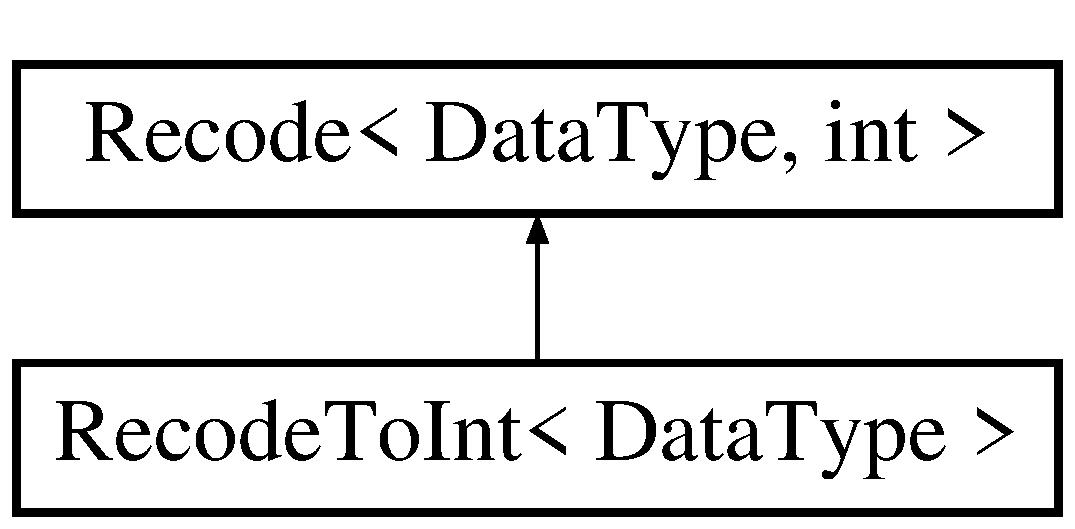
\includegraphics[height=2cm]{class_recode_to_int}
\end{center}
\end{figure}
\subsection*{Public Member Functions}
\begin{CompactItemize}
\item 
{\bf Recode\-To\-Int} ()\label{class_recode_to_int_7afccf5cc723177c720d62d7eedc5414}

\begin{CompactList}\small\item\em Contructor. \item\end{CompactList}\item 
template$<$class Container$>$ {\bf Recode\-To\-Int} (Container \&itemset)
\begin{CompactList}\small\item\em Contructor used to construct the recode object initialized with a SET (not a multi set) of Data\-Type. \item\end{CompactList}\item 
virtual {\bf $\sim$Recode\-To\-Int} ()\label{class_recode_to_int_264d862332a6695baeeb1625d22b8434}

\begin{CompactList}\small\item\em Destructor. \item\end{CompactList}\item 
{\bf Recode\-To\-Int} (const {\bf Recode\-To\-Int} \&rec)\label{class_recode_to_int_8ae90856c152323463a232005e5fb878}

\begin{CompactList}\small\item\em Copy contructor. \item\end{CompactList}\item 
{\bf Recode\-To\-Int} \& {\bf operator=} (const {\bf Recode\-To\-Int} \&rec)\label{class_recode_to_int_40bf1ee6b8a5e79af7a688b3b59eb009}

\begin{CompactList}\small\item\em Affectation operator. \item\end{CompactList}\item 
template$<$class Container$>$ vector$<$ int $>$ \& {\bf operator()} (Container \&itemset)
\begin{CompactList}\small\item\em Map elements of the input data in internals ids. \item\end{CompactList}\item 
template$<$class Input\-Iterator$>$ vector$<$ int $>$ \& {\bf operator()} (Input\-Iterator first, Input\-Iterator last)
\begin{CompactList}\small\item\em Map elements of the input data in internals ids. \item\end{CompactList}\item 
virtual int {\bf operator()} (Data\-Type item)
\begin{CompactList}\small\item\em Map an element of the input data in an internals id. \item\end{CompactList}\item 
template$<$class Container$>$ vector$<$ Data\-Type $>$ \& {\bf remap} (Container \&itemset)
\begin{CompactList}\small\item\em Remap internals ids in elements of the input data . \item\end{CompactList}\item 
void {\bf remap} (vector$<$ int $>$ $\ast$itemset, vector$<$ Data\-Type $>$ $\ast$remap\-Itemsets)
\begin{CompactList}\small\item\em Remap internals set of ids in the corresponfing set of elements of the input data . \item\end{CompactList}\item 
template$<$class Input\-Iterator$>$ vector$<$ Data\-Type $>$ \& {\bf remap} (Input\-Iterator first, Input\-Iterator last)
\begin{CompactList}\small\item\em Remap internals ids in elements of the input data . \item\end{CompactList}\item 
virtual Data\-Type {\bf remap} (int item)
\begin{CompactList}\small\item\em Map an element of the input data in an internals id. \item\end{CompactList}\end{CompactItemize}
\subsection*{Public Attributes}
\begin{CompactItemize}
\item 
vector$<$ Data\-Type $>$ {\bf int\-Id\-Toid}\label{class_recode_to_int_0286413c937d57bc153465e4c7625d6c}

\begin{CompactList}\small\item\em vector used to map the internal id to the real elemnt. \item\end{CompactList}\end{CompactItemize}


\subsection{Detailed Description}
\subsubsection*{template$<$class Data\-Type$>$ class Recode\-To\-Int$<$ Data\-Type $>$}

Class {\bf Recode\-To\-Int}{\rm (p.\,\pageref{class_recode_to_int})} recode data oftype T in integers and stor the mapping. 

The template parameter is the original type of the elements to recode in int. The internal id of the element are defined wrt the order they are passed to the functor. For example the first element passed to the functor have the id 0, the second element 1,... 



\subsection{Constructor \& Destructor Documentation}
\index{RecodeToInt@{Recode\-To\-Int}!RecodeToInt@{RecodeToInt}}
\index{RecodeToInt@{RecodeToInt}!RecodeToInt@{Recode\-To\-Int}}
\subsubsection{\setlength{\rightskip}{0pt plus 5cm}template$<$class Data\-Type$>$ template$<$class Container$>$ {\bf Recode\-To\-Int}$<$ Data\-Type $>$::{\bf Recode\-To\-Int} (Container \& {\em itemset})\hspace{0.3cm}{\tt  [inline]}}\label{class_recode_to_int_c79659f9e5d7b2a894cb9edaed32b32d}


Contructor used to construct the recode object initialized with a SET (not a multi set) of Data\-Type. 

Since recode is empty, the sets are new sets to recode, there is no need to search if they already recoded. 

\subsection{Member Function Documentation}
\index{RecodeToInt@{Recode\-To\-Int}!operator()@{operator()}}
\index{operator()@{operator()}!RecodeToInt@{Recode\-To\-Int}}
\subsubsection{\setlength{\rightskip}{0pt plus 5cm}template$<$class Data\-Type$>$ int {\bf Recode\-To\-Int}$<$ Data\-Type $>$::operator() (Data\-Type {\em item})\hspace{0.3cm}{\tt  [virtual]}}\label{class_recode_to_int_84e738bd2a7faf92a7d916e995689cab}


Map an element of the input data in an internals id. 

\begin{Desc}
\item[Returns:]the new id. \end{Desc}


Implements {\bf Recode$<$ Data\-Type, int $>$} {\rm (p.\,\pageref{class_recode_266e8a09b4576e02aab3cd6590a9ffbf})}.\index{RecodeToInt@{Recode\-To\-Int}!operator()@{operator()}}
\index{operator()@{operator()}!RecodeToInt@{Recode\-To\-Int}}
\subsubsection{\setlength{\rightskip}{0pt plus 5cm}template$<$class Data\-Type$>$ template$<$class Input\-Iterator$>$ vector$<$ int $>$ \& {\bf Recode\-To\-Int}$<$ Data\-Type $>$::operator() (Input\-Iterator {\em first}, Input\-Iterator {\em last})}\label{class_recode_to_int_51f3193e2ace542f3041ee0f3dca8deb}


Map elements of the input data in internals ids. 

\begin{Desc}
\item[Parameters:]
\begin{description}
\item[{\em first}]iterator on the first element \item[{\em last}]iterator on the element after the last \end{description}
\end{Desc}
\begin{Desc}
\item[Returns:]the new ids. \end{Desc}
\index{RecodeToInt@{Recode\-To\-Int}!operator()@{operator()}}
\index{operator()@{operator()}!RecodeToInt@{Recode\-To\-Int}}
\subsubsection{\setlength{\rightskip}{0pt plus 5cm}template$<$class Data\-Type$>$ template$<$class Container$>$ vector$<$ int $>$ \& {\bf Recode\-To\-Int}$<$ Data\-Type $>$::operator() (Container \& {\em itemset})}\label{class_recode_to_int_7d3d3ea423abd8e055ba4483744fba04}


Map elements of the input data in internals ids. 

\begin{Desc}
\item[Parameters:]
\begin{description}
\item[{\em itemset}]set of elements to recode in int. \end{description}
\end{Desc}
\begin{Desc}
\item[Returns:]the new ids. \end{Desc}


Reimplemented from {\bf Recode$<$ Data\-Type, int $>$} {\rm (p.\,\pageref{class_recode_d4fc62868c9f2097c762a6e0c66ae685})}.\index{RecodeToInt@{Recode\-To\-Int}!remap@{remap}}
\index{remap@{remap}!RecodeToInt@{Recode\-To\-Int}}
\subsubsection{\setlength{\rightskip}{0pt plus 5cm}template$<$class Data\-Type$>$ virtual Data\-Type {\bf Recode\-To\-Int}$<$ Data\-Type $>$::remap (int {\em item})\hspace{0.3cm}{\tt  [inline, virtual]}}\label{class_recode_to_int_338aeadf35cd3aad00d61d313bdf59d2}


Map an element of the input data in an internals id. 

\begin{Desc}
\item[Returns:]the new id. \end{Desc}
\index{RecodeToInt@{Recode\-To\-Int}!remap@{remap}}
\index{remap@{remap}!RecodeToInt@{Recode\-To\-Int}}
\subsubsection{\setlength{\rightskip}{0pt plus 5cm}template$<$class Data\-Type$>$ template$<$class Input\-Iterator$>$ vector$<$Data\-Type$>$\& {\bf Recode\-To\-Int}$<$ Data\-Type $>$::remap (Input\-Iterator {\em first}, Input\-Iterator {\em last})\hspace{0.3cm}{\tt  [inline]}}\label{class_recode_to_int_a138eafdc7693c0cf5057c6fc786d80b}


Remap internals ids in elements of the input data . 

\begin{Desc}
\item[Parameters:]
\begin{description}
\item[{\em first}]iterator on the first element to remap. \item[{\em last}]iterator on the element after the last to remap. \end{description}
\end{Desc}
\begin{Desc}
\item[Returns:]the original ids. \end{Desc}
\index{RecodeToInt@{Recode\-To\-Int}!remap@{remap}}
\index{remap@{remap}!RecodeToInt@{Recode\-To\-Int}}
\subsubsection{\setlength{\rightskip}{0pt plus 5cm}template$<$class Data\-Type$>$ void {\bf Recode\-To\-Int}$<$ Data\-Type $>$::remap (vector$<$ int $>$ $\ast$ {\em itemset}, vector$<$ Data\-Type $>$ $\ast$ {\em remap\-Itemsets})\hspace{0.3cm}{\tt  [inline]}}\label{class_recode_to_int_8dcffed515a66b6a64c837933dca615e}


Remap internals set of ids in the corresponfing set of elements of the input data . 

\begin{Desc}
\item[Parameters:]
\begin{description}
\item[{\em itemset}]set of elements to recode in input Data type. \item[{\em remap\-Itemsets}]for the original ids . \end{description}
\end{Desc}
\index{RecodeToInt@{Recode\-To\-Int}!remap@{remap}}
\index{remap@{remap}!RecodeToInt@{Recode\-To\-Int}}
\subsubsection{\setlength{\rightskip}{0pt plus 5cm}template$<$class Data\-Type$>$ template$<$class Container$>$ vector$<$Data\-Type$>$\& {\bf Recode\-To\-Int}$<$ Data\-Type $>$::remap (Container \& {\em itemset})\hspace{0.3cm}{\tt  [inline]}}\label{class_recode_to_int_814de08675679f300ae7171f560b0e61}


Remap internals ids in elements of the input data . 

\begin{Desc}
\item[Parameters:]
\begin{description}
\item[{\em itemset}]set of elements to recode in input Data type. \end{description}
\end{Desc}
\begin{Desc}
\item[Returns:]the original ids . \end{Desc}


The documentation for this class was generated from the following file:\begin{CompactItemize}
\item 
F:/i\-Zi/util/Recode\-To\-Int.hxx\end{CompactItemize}

\section{Record\-Distribution$<$ Output $>$ Class Template Reference}
\label{class_record_distribution}\index{RecordDistribution@{RecordDistribution}}
Class used to store the distribution of a solution find by an algorithm (and evantually save the solution in an output object).  


{\tt \#include $<$Record\-Distribution.hxx$>$}

\subsection*{Public Member Functions}
\begin{CompactItemize}
\item 
{\bf Record\-Distribution} (Output $\ast$inobjectwrapped=0)\label{class_record_distribution_3a21d8d0c0f191202986d518ed1fcf49}

\begin{CompactList}\small\item\em Constructor. \item\end{CompactList}\item 
virtual {\bf $\sim$Record\-Distribution} ()\label{class_record_distribution_5b8461d785ece13a14f24163b086b340}

\begin{CompactList}\small\item\em Destructor. \item\end{CompactList}\item 
vector$<$ int $>$ \& {\bf distribution} ()\label{class_record_distribution_d116898ebb6a753623e55f89063aaf53}

\begin{CompactList}\small\item\em Function to access the container storing the ditribution. \item\end{CompactList}\item 
template$<$class Container, class Measure$>$ void {\bf push\_\-back} (Container \&set\-Element, Measure measure)
\begin{CompactList}\small\item\em Function called when a solution is find, and used to store informations and eventually store the solution in another output object. \item\end{CompactList}\item 
template$<$class Container$>$ void {\bf push\_\-back} (Container \&set\-Element, {\bf Boolean} measure)
\begin{CompactList}\small\item\em Function called when a solution is find. \item\end{CompactList}\item 
template$<$class Container$>$ void {\bf push\_\-back} (Container \&set\-Element)
\begin{CompactList}\small\item\em Function called when a solution is find, and used to store informations and eventually store the solution in another output object. \item\end{CompactList}\item 
template$<$class Input\-Iterator, class Measure$>$ void {\bf push\_\-back} (Input\-Iterator first, Input\-Iterator last, Measure measure)
\begin{CompactList}\small\item\em Function called when a solution is find, and used to store informations and eventually store the solution in another output object. \item\end{CompactList}\item 
int {\bf size} ()\label{class_record_distribution_df406703f289b76e764dbb11f17442e7}

\begin{CompactList}\small\item\em Get the number of levels studied. \item\end{CompactList}\item 
int \& {\bf operator[$\,$]} (const int \&i)\label{class_record_distribution_a6a9e7b9f8bae800c8c1fdd12b402b91}

\begin{CompactList}\small\item\em Access the number elements of size i. \item\end{CompactList}\end{CompactItemize}
\subsection*{Protected Attributes}
\begin{CompactItemize}
\item 
vector$<$ int $>$ {\bf distrib}\label{class_record_distribution_bef4620c1ab9333fea93eb5811c8b2d3}

\begin{CompactList}\small\item\em distribution of the elements of the solution \item\end{CompactList}\item 
Output $\ast$ {\bf objectwrapped}\label{class_record_distribution_e4b17eb76d6b043a0d8e637c901d3b69}

\begin{CompactList}\small\item\em Pointer on the ouput object wrapped. \item\end{CompactList}\end{CompactItemize}


\subsection{Detailed Description}
\subsubsection*{template$<$class Output = No\-Output$>$ class Record\-Distribution$<$ Output $>$}

Class used to store the distribution of a solution find by an algorithm (and evantually save the solution in an output object). 

The objects of this class are passed in parameter of the algorithm by using the output parameters. For example, suppose that we have an algorithm that process the theory of a language. This algorithm will have at least 3 parameters: the initialization functor of the language, the predicate and an object to output the theory. This output object could be a file, a data structure or a \char`\"{}statistical\char`\"{} object that records some informations about the elements of the solution. The current class is such a \char`\"{}statistical\char`\"{} output class, and it is used to store the distribution of the elements of the solution, ie the number of elements wrt to their size. Since it should be possible to record stat and save solution in a file or a dat structure, this class could be a wrapper to such objects. This way this class could record informations and save solutions in the output object wrapped at the same time and transparently.. 



\subsection{Member Function Documentation}
\index{RecordDistribution@{Record\-Distribution}!push_back@{push\_\-back}}
\index{push_back@{push\_\-back}!RecordDistribution@{Record\-Distribution}}
\subsubsection{\setlength{\rightskip}{0pt plus 5cm}template$<$class Output = No\-Output$>$ template$<$class Input\-Iterator, class Measure$>$ void {\bf Record\-Distribution}$<$ Output $>$::push\_\-back (Input\-Iterator {\em first}, Input\-Iterator {\em last}, Measure {\em measure})\hspace{0.3cm}{\tt  [inline]}}\label{class_record_distribution_cbe7f0b5cc0f3a0b8f377dfa458f29dd}


Function called when a solution is find, and used to store informations and eventually store the solution in another output object. 

The template parameter represents the input iterators on the integers to insert in the file. \begin{Desc}
\item[Parameters:]
\begin{description}
\item[{\em first}]iterator on the first element. \item[{\em last}]iterator on the element after the last. \item[{\em measure}]additional measure assoiated with the element. \end{description}
\end{Desc}
\index{RecordDistribution@{Record\-Distribution}!push_back@{push\_\-back}}
\index{push_back@{push\_\-back}!RecordDistribution@{Record\-Distribution}}
\subsubsection{\setlength{\rightskip}{0pt plus 5cm}template$<$class Output = No\-Output$>$ template$<$class Container$>$ void {\bf Record\-Distribution}$<$ Output $>$::push\_\-back (Container \& {\em set\-Element})\hspace{0.3cm}{\tt  [inline]}}\label{class_record_distribution_de2a7208d4488d81d383f10965b34cff}


Function called when a solution is find, and used to store informations and eventually store the solution in another output object. 

This function corresponds to the classic {\bf push\_\-back( )}{\rm (p.\,\pageref{class_record_distribution_68c52a30268722a731552ee98657f761})} function od STL container. The template parameter represents a container of elements. \begin{Desc}
\item[Parameters:]
\begin{description}
\item[{\em set\-Element}]the set of element to insert in the file. \item[{\em measure}]additional measure assoiated with the element. \end{description}
\end{Desc}
\index{RecordDistribution@{Record\-Distribution}!push_back@{push\_\-back}}
\index{push_back@{push\_\-back}!RecordDistribution@{Record\-Distribution}}
\subsubsection{\setlength{\rightskip}{0pt plus 5cm}template$<$class Output = No\-Output$>$ template$<$class Container$>$ void {\bf Record\-Distribution}$<$ Output $>$::push\_\-back (Container \& {\em set\-Element}, {\bf Boolean} {\em measure})\hspace{0.3cm}{\tt  [inline]}}\label{class_record_distribution_1ded57b0d84d851147c160e44036a05e}


Function called when a solution is find. 

This function corresponds to the classic {\bf push\_\-back( )}{\rm (p.\,\pageref{class_record_distribution_68c52a30268722a731552ee98657f761})} function od STL container. The template parameter represents a container of elements. \begin{Desc}
\item[Parameters:]
\begin{description}
\item[{\em set\-Element}]the set of element to insert in the file. \end{description}
\end{Desc}
\index{RecordDistribution@{Record\-Distribution}!push_back@{push\_\-back}}
\index{push_back@{push\_\-back}!RecordDistribution@{Record\-Distribution}}
\subsubsection{\setlength{\rightskip}{0pt plus 5cm}template$<$class Output = No\-Output$>$ template$<$class Container, class Measure$>$ void {\bf Record\-Distribution}$<$ Output $>$::push\_\-back (Container \& {\em set\-Element}, Measure {\em measure})\hspace{0.3cm}{\tt  [inline]}}\label{class_record_distribution_68c52a30268722a731552ee98657f761}


Function called when a solution is find, and used to store informations and eventually store the solution in another output object. 

This function corresponds to the classic {\bf push\_\-back( )}{\rm (p.\,\pageref{class_record_distribution_68c52a30268722a731552ee98657f761})} function od STL container. The template parameter represents a container of elements. \begin{Desc}
\item[Parameters:]
\begin{description}
\item[{\em set\-Element}]the set of element to insert in the file. \item[{\em measure}]additional measure assoiated with the element. \end{description}
\end{Desc}


The documentation for this class was generated from the following file:\begin{CompactItemize}
\item 
F:/i\-Zi/util/Record\-Distribution.hxx\end{CompactItemize}

\section{Satisfied\-IND$<$ Data $>$ Class Template Reference}
\label{class_satisfied_i_n_d}\index{SatisfiedIND@{SatisfiedIND}}
Functor representing the predicate being a satisfied {\bf IND}{\rm (p.\,\pageref{class_i_n_d})} wrt to 2 relations.  


{\tt \#include $<$Satisfied\-IND.hxx$>$}

Inheritance diagram for Satisfied\-IND$<$ Data $>$::\begin{figure}[H]
\begin{center}
\leavevmode
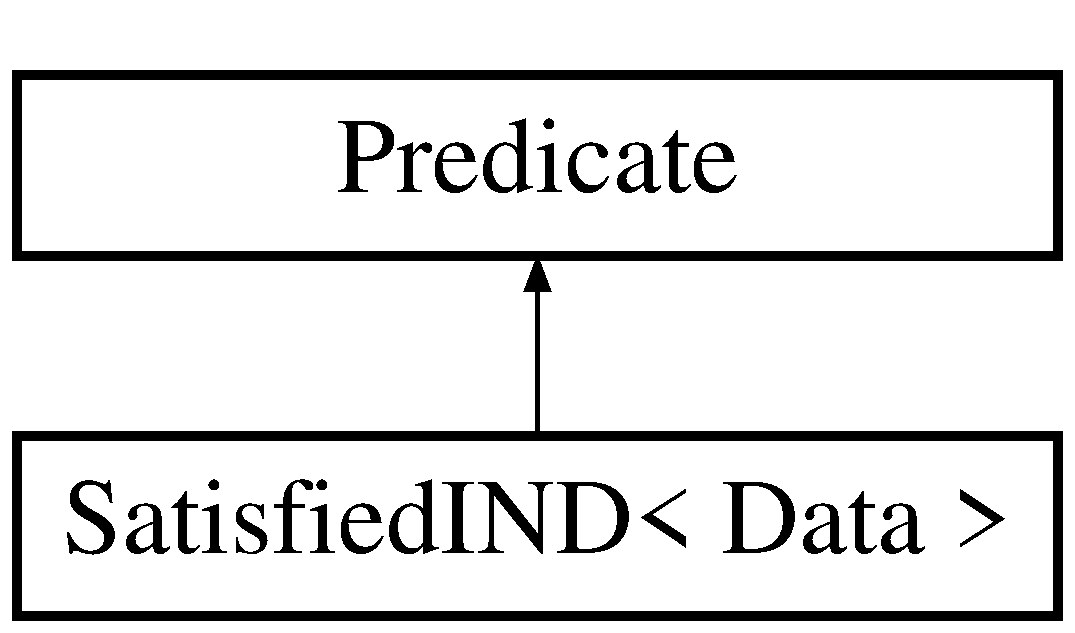
\includegraphics[height=2cm]{class_satisfied_i_n_d}
\end{center}
\end{figure}
\subsection*{Public Member Functions}
\begin{CompactItemize}
\item 
template$<$class Input\-DBFormat$>$ {\bf Satisfied\-IND} (Data \&intable1, Input\-DBFormat \&input1, Data \&intable2, Input\-DBFormat \&input2)
\begin{CompactList}\small\item\em Constructor. \item\end{CompactList}\item 
{\bf $\sim$Satisfied\-IND} ()\label{class_satisfied_i_n_d_42ee5fbb4365e4ebaa5b6d2811cd90a5}

\begin{CompactList}\small\item\em Destructor. \item\end{CompactList}\item 
template$<$class Iterator, class Measure$>$ bool {\bf operator()} (Iterator it\-Cand, Measure \&mes\-Cand)
\begin{CompactList}\small\item\em Operator that test if a set of attributes is a satisfied {\bf IND}{\rm (p.\,\pageref{class_i_n_d})}. \item\end{CompactList}\end{CompactItemize}
\subsection*{Protected Member Functions}
\begin{CompactItemize}
\item 
template$<$class Container\-Attrib, class Container\-Project$>$ void {\bf projection} (Data $\ast$relation, Container\-Attrib \&set\-Of\-Attrib, Container\-Project \&project, {\bf Recode\-To\-Int}$<$ string $>$ \&num\-Attrib)
\begin{CompactList}\small\item\em function used to project a relation wrt a set of attributes. \item\end{CompactList}\end{CompactItemize}
\subsection*{Protected Attributes}
\begin{CompactItemize}
\item 
Data $\ast$ {\bf table1}\label{class_satisfied_i_n_d_40870e6e2f4d671c3658f4e9d9775b70}

\begin{CompactList}\small\item\em the first relation 1 \item\end{CompactList}\item 
Data $\ast$ {\bf table2}\label{class_satisfied_i_n_d_067ee67848d21e1bc5f04f1531e60a51}

\begin{CompactList}\small\item\em the first relation 2 \item\end{CompactList}\item 
{\bf Recode\-To\-Int}$<$ string $>$ {\bf num\-Attrib1}\label{class_satisfied_i_n_d_2e89ec65c6746fba9dc90eda29197867}

\begin{CompactList}\small\item\em Used to get the numero of the attributes ( 1st, 2nd,...) of the first relation. \item\end{CompactList}\item 
{\bf Recode\-To\-Int}$<$ string $>$ {\bf num\-Attrib2}\label{class_satisfied_i_n_d_01f0ff69e35875dbc6b9c02f7b514fc4}

\begin{CompactList}\small\item\em Used to get the numero of the attributes ( 1st, 2nd,...) of the first relation. \item\end{CompactList}\end{CompactItemize}
\subsection*{Classes}
\begin{CompactItemize}
\item 
class {\bf Process\-Tuples}
\begin{CompactList}\small\item\em Functor used to projet all the tuples wrt attributes studied. \item\end{CompactList}\item 
class {\bf project2}
\begin{CompactList}\small\item\em Functor used to projet a tuple wrt the set of attributes studied. \item\end{CompactList}\end{CompactItemize}


\subsection{Detailed Description}
\subsubsection*{template$<$class Data$>$ class Satisfied\-IND$<$ Data $>$}

Functor representing the predicate being a satisfied {\bf IND}{\rm (p.\,\pageref{class_i_n_d})} wrt to 2 relations. 

This functor test if a {\bf IND}{\rm (p.\,\pageref{class_i_n_d})} is satisfied. The method used to test if a candidate is a a satisfied {\bf IND}{\rm (p.\,\pageref{class_i_n_d})} is the following one: process the projection wrt the attributes of the left side of the candidate {\bf IND}{\rm (p.\,\pageref{class_i_n_d})}. process the projection wrt the attributes of the right side of the candidate {\bf IND}{\rm (p.\,\pageref{class_i_n_d})}. check that each element of left side projection is included in the right side projection. return true if all the element are included.

The template parameter Data is the type of the tablular data. 



\subsection{Constructor \& Destructor Documentation}
\index{SatisfiedIND@{Satisfied\-IND}!SatisfiedIND@{SatisfiedIND}}
\index{SatisfiedIND@{SatisfiedIND}!SatisfiedIND@{Satisfied\-IND}}
\subsubsection{\setlength{\rightskip}{0pt plus 5cm}template$<$class Data$>$ template$<$class Input\-DBFormat$>$ {\bf Satisfied\-IND}$<$ Data $>$::{\bf Satisfied\-IND} (Data \& {\em intable1}, Input\-DBFormat \& {\em input1}, Data \& {\em intable2}, Input\-DBFormat \& {\em input2})\hspace{0.3cm}{\tt  [inline]}}\label{class_satisfied_i_n_d_083227d8e372ee6954f7e11e5c84d4bc}


Constructor. 

\begin{Desc}
\item[Parameters:]
\begin{description}
\item[{\em intable1}]data of the first relation/table studied \item[{\em input1}]file containing the first relation/table studied \item[{\em intable2}]data of the second relation/table studied \item[{\em input2}]file containing the second relation/table studied \end{description}
\end{Desc}


\subsection{Member Function Documentation}
\index{SatisfiedIND@{Satisfied\-IND}!operator()@{operator()}}
\index{operator()@{operator()}!SatisfiedIND@{Satisfied\-IND}}
\subsubsection{\setlength{\rightskip}{0pt plus 5cm}template$<$class Data$>$ template$<$class Iterator, class Measure$>$ bool {\bf Satisfied\-IND}$<$ Data $>$::operator() (Iterator {\em it\-Cand}, Measure \& {\em mes\-Cand})}\label{class_satisfied_i_n_d_bbf69fd5dfbf71f8e7f0685b80551c6d}


Operator that test if a set of attributes is a satisfied {\bf IND}{\rm (p.\,\pageref{class_i_n_d})}. 

\begin{Desc}
\item[Parameters:]
\begin{description}
\item[{\em it\-Cand}]iterator (or pointer) on the set of attributes to test wrt the predicate \item[{\em mes\-Cand}]cardinality of the projection on the db of the attributes \end{description}
\end{Desc}


Reimplemented from {\bf Predicate} {\rm (p.\,\pageref{class_predicate_6fb1a75dba2268f75738f335f403e46c})}.\index{SatisfiedIND@{Satisfied\-IND}!projection@{projection}}
\index{projection@{projection}!SatisfiedIND@{Satisfied\-IND}}
\subsubsection{\setlength{\rightskip}{0pt plus 5cm}template$<$class Data$>$ template$<$class Container\-Attrib, class Container\-Project$>$ void {\bf Satisfied\-IND}$<$ Data $>$::projection (Data $\ast$ {\em relation}, Container\-Attrib \& {\em set\-Of\-Attrib}, Container\-Project \& {\em project}, {\bf Recode\-To\-Int}$<$ string $>$ \& {\em num\-Attrib})\hspace{0.3cm}{\tt  [protected]}}\label{class_satisfied_i_n_d_bb4eeaeb80e39c8e6dcc804444a1c44e}


function used to project a relation wrt a set of attributes. 

\begin{Desc}
\item[Parameters:]
\begin{description}
\item[{\em relation}]class representing the relation. \item[{\em Container\-Attrib}]set of attribute used for the projection. \item[{\em Container\-Project}]container used to store the projection. \end{description}
\end{Desc}


The documentation for this class was generated from the following file:\begin{CompactItemize}
\item 
F:/i\-Zi/problems/DI/Satisfied\-IND.hxx\end{CompactItemize}

\section{Satisfied\-IND$<$ Data $>$::Process\-Tuples$<$ Container\-Attrib, Container\-Project $>$ Class Template Reference}
\label{class_satisfied_i_n_d_1_1_process_tuples}\index{SatisfiedIND::ProcessTuples@{SatisfiedIND::ProcessTuples}}
Functor used to projet all the tuples wrt attributes studied.  


{\tt \#include $<$Satisfied\-IND.hxx$>$}



\subsection{Detailed Description}
\subsubsection*{template$<$class Data$>$template$<$class Container\-Attrib, class Container\-Project$>$ class Satisfied\-IND$<$ Data $>$::Process\-Tuples$<$ Container\-Attrib, Container\-Project $>$}

Functor used to projet all the tuples wrt attributes studied. 



The documentation for this class was generated from the following file:\begin{CompactItemize}
\item 
F:/i\-Zi/problems/DI/Satisfied\-IND.hxx\end{CompactItemize}

\section{Satisfied\-IND$<$ Data $>$::project2$<$ Container\-Tuple $>$ Class Template Reference}
\label{class_satisfied_i_n_d_1_1project2}\index{SatisfiedIND::project2@{SatisfiedIND::project2}}
Functor used to projet a tuple wrt the set of attributes studied.  


{\tt \#include $<$Satisfied\-IND.hxx$>$}



\subsection{Detailed Description}
\subsubsection*{template$<$class Data$>$template$<$class Container\-Tuple$>$ class Satisfied\-IND$<$ Data $>$::project2$<$ Container\-Tuple $>$}

Functor used to projet a tuple wrt the set of attributes studied. 



The documentation for this class was generated from the following file:\begin{CompactItemize}
\item 
F:/i\-Zi/problems/DI/Satisfied\-IND.hxx\end{CompactItemize}

\section{Satisfied\-IND\_\-DBMS$<$ DBMS $>$ Class Template Reference}
\label{class_satisfied_i_n_d___d_b_m_s}\index{SatisfiedIND_DBMS@{SatisfiedIND\_\-DBMS}}
Functor representing the predicate being a satisfied {\bf IND}{\rm (p.\,\pageref{class_i_n_d})} wrt to 2 relations in a SGBD.  


{\tt \#include $<$Satisfied\-IND\_\-DBMS.hxx$>$}

Inheritance diagram for Satisfied\-IND\_\-DBMS$<$ DBMS $>$::\begin{figure}[H]
\begin{center}
\leavevmode
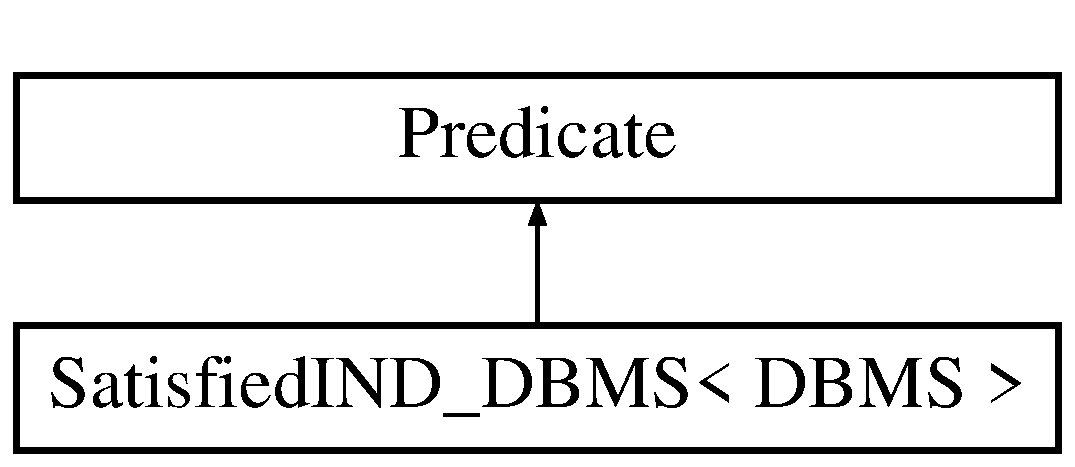
\includegraphics[height=2cm]{class_satisfied_i_n_d___d_b_m_s}
\end{center}
\end{figure}
\subsection*{Public Member Functions}
\begin{CompactItemize}
\item 
{\bf Satisfied\-IND\_\-DBMS} (DBMS $\ast$in\-Dbms)
\begin{CompactList}\small\item\em Constructor. \item\end{CompactList}\item 
{\bf $\sim$Satisfied\-IND\_\-DBMS} ()\label{class_satisfied_i_n_d___d_b_m_s_26071485b5e3be1fb328fe4cc1a9a336}

\begin{CompactList}\small\item\em Destructor. \item\end{CompactList}\item 
template$<$class Iterator, class Measure$>$ bool {\bf operator()} (Iterator it\-Cand, Measure \&mes\-Cand)\label{class_satisfied_i_n_d___d_b_m_s_10cb098e49804f3de10b20c1d3317814}

\begin{CompactList}\small\item\em Operator that test if a set of attributes is not redundant. \item\end{CompactList}\end{CompactItemize}
\subsection*{Protected Attributes}
\begin{CompactItemize}
\item 
DBMS $\ast$ {\bf mydbms}\label{class_satisfied_i_n_d___d_b_m_s_6a69c4a2896c294ee5bb98959f1775bc}

\begin{CompactList}\small\item\em Pointer on the dbms. \item\end{CompactList}\end{CompactItemize}


\subsection{Detailed Description}
\subsubsection*{template$<$class DBMS$>$ class Satisfied\-IND\_\-DBMS$<$ DBMS $>$}

Functor representing the predicate being a satisfied {\bf IND}{\rm (p.\,\pageref{class_i_n_d})} wrt to 2 relations in a SGBD. 

This functor test if a {\bf IND}{\rm (p.\,\pageref{class_i_n_d})} is satisfied for two relation stored in a DBMS. Note that each time the functor is used, a query is executed on the database.

The template parameter DBMS is the class representing the connection to the DBMS. This class is used to do operations on the DBMS such as connect, execute a query ...

The attributes in the two relations must have the same data type. 



\subsection{Constructor \& Destructor Documentation}
\index{SatisfiedIND_DBMS@{Satisfied\-IND\_\-DBMS}!SatisfiedIND_DBMS@{SatisfiedIND\_\-DBMS}}
\index{SatisfiedIND_DBMS@{SatisfiedIND\_\-DBMS}!SatisfiedIND_DBMS@{Satisfied\-IND\_\-DBMS}}
\subsubsection{\setlength{\rightskip}{0pt plus 5cm}template$<$class DBMS$>$ {\bf Satisfied\-IND\_\-DBMS}$<$ DBMS $>$::{\bf Satisfied\-IND\_\-DBMS} (DBMS $\ast$ {\em in\-Dbms})\hspace{0.3cm}{\tt  [inline]}}\label{class_satisfied_i_n_d___d_b_m_s_90330aefbc693768d516a523f4f04625}


Constructor. 

\begin{Desc}
\item[Parameters:]
\begin{description}
\item[{\em in\-Dbms}]pointer on the DBMS and the database studied \end{description}
\end{Desc}


The documentation for this class was generated from the following file:\begin{CompactItemize}
\item 
F:/i\-Zi/problems/DI/Satisfied\-IND\_\-DBMS.hxx\end{CompactItemize}

\section{save\-Container Class Reference}
\label{classsave_container}\index{saveContainer@{saveContainer}}
Functor used to save the data of a container in a file.  


{\tt \#include $<$Recode\-To\-Int.hxx$>$}



\subsection{Detailed Description}
Functor used to save the data of a container in a file. 



The documentation for this class was generated from the following file:\begin{CompactItemize}
\item 
F:/i\-Zi/util/Recode\-To\-Int.hxx\end{CompactItemize}

\section{save\-Container\-Of\-Container Class Reference}
\label{classsave_container_of_container}\index{saveContainerOfContainer@{saveContainerOfContainer}}
Functor used to save the data of a container of container.  


{\tt \#include $<$Recode\-To\-Int.hxx$>$}



\subsection{Detailed Description}
Functor used to save the data of a container of container. 



The documentation for this class was generated from the following file:\begin{CompactItemize}
\item 
F:/i\-Zi/util/Recode\-To\-Int.hxx\end{CompactItemize}

\section{Stop\-Ite\-Distrib Class Reference}
\label{class_stop_ite_distrib}\index{StopIteDistrib@{StopIteDistrib}}
Functor used in parameter of {\bf Apriori}{\rm (p.\,\pageref{class_apriori})} to stop the execution of the algorithm wrt distribution of elements found.  


{\tt \#include $<$Stop\-Ite\-Distrib.hxx$>$}

\subsection*{Public Member Functions}
\begin{CompactItemize}
\item 
{\bf Stop\-Ite\-Distrib} (int inthreshold)\label{class_stop_ite_distrib_2a09ac7b4eb5215720e4e704085dc356}

\begin{CompactList}\small\item\em Constructor. \item\end{CompactList}\item 
template$<$class Cand\_\-Data\-Struct$>$ void {\bf update} (Cand\_\-Data\-Struct \&candidates)
\begin{CompactList}\small\item\em Update the informations in the functor wrt the current step of the algorithme. \item\end{CompactList}\item 
template$<$class Cand\_\-Data\-Struct$>$ bool {\bf operator()} (Cand\_\-Data\-Struct \&candidates)
\begin{CompactList}\small\item\em Operator used to determine if the algorithm should stop. \item\end{CompactList}\end{CompactItemize}
\subsection*{Public Attributes}
\begin{CompactItemize}
\item 
int {\bf level}\label{class_stop_ite_distrib_4e439159feb6fb1117a9b5ca471121ca}

\begin{CompactList}\small\item\em Last level studied by the algorithm. \item\end{CompactList}\end{CompactItemize}
\subsection*{Protected Attributes}
\begin{CompactItemize}
\item 
int {\bf threshold}\label{class_stop_ite_distrib_c26278c24bbfe949fb0010be2b32b170}

\begin{CompactList}\small\item\em threshold (if $>$ 1 last level studied). \item\end{CompactList}\item 
int {\bf nb\-Cand}\label{class_stop_ite_distrib_0c03770bf116aab0df9410be57e94e61}

\begin{CompactList}\small\item\em Number of candidates for the current level at th curretn step of the algorithm. \item\end{CompactList}\end{CompactItemize}


\subsection{Detailed Description}
Functor used in parameter of {\bf Apriori}{\rm (p.\,\pageref{class_apriori})} to stop the execution of the algorithm wrt distribution of elements found. 

If the threshold is less or equal than 1, stop the {\bf Apriori}{\rm (p.\,\pageref{class_apriori})} execution when the number of elments in the negative border found in an iteration on the number of candidates generated is less than a threshold given in input. If the threshold is greater than 1, stop when the algorithm has processed level = threshold. 



\subsection{Member Function Documentation}
\index{StopIteDistrib@{Stop\-Ite\-Distrib}!operator()@{operator()}}
\index{operator()@{operator()}!StopIteDistrib@{Stop\-Ite\-Distrib}}
\subsubsection{\setlength{\rightskip}{0pt plus 5cm}template$<$class Cand\_\-Data\-Struct$>$ bool Stop\-Ite\-Distrib::operator() (Cand\_\-Data\-Struct \& {\em candidates})\hspace{0.3cm}{\tt  [inline]}}\label{class_stop_ite_distrib_d6386032f32f664ed1b4813b3a645b62}


Operator used to determine if the algorithm should stop. 

Since the test is done after the pruning step of {\bf Apriori}{\rm (p.\,\pageref{class_apriori})}, we store \begin{Desc}
\item[Returns:]true if the ratio on the number of elements of Bd- on the numbre of candidates generated is less thant the thresold. \end{Desc}
\index{StopIteDistrib@{Stop\-Ite\-Distrib}!update@{update}}
\index{update@{update}!StopIteDistrib@{Stop\-Ite\-Distrib}}
\subsubsection{\setlength{\rightskip}{0pt plus 5cm}template$<$class Cand\_\-Data\-Struct$>$ void Stop\-Ite\-Distrib::update (Cand\_\-Data\-Struct \& {\em candidates})\hspace{0.3cm}{\tt  [inline]}}\label{class_stop_ite_distrib_70910a2a1fd59c7ba5873088891e4d2b}


Update the informations in the functor wrt the current step of the algorithme. 

By updating the informations in the functor we consider the informations discovered at another step of the algorithm. For example, an update is done in {\bf Apriori}{\rm (p.\,\pageref{class_apriori})} after generating (+ pre processing of the predicate) candidates. 

The documentation for this class was generated from the following file:\begin{CompactItemize}
\item 
F:/i\-Zi/algorithms/Stop\-Ite\-Distrib.hxx\end{CompactItemize}

\section{Support Class Reference}
\label{class_support}\index{Support@{Support}}
Class used to store additional informations in each node, here the support of the corresponding items.  


{\tt \#include $<$Support.hpp$>$}

Inheritance diagram for Support::\begin{figure}[H]
\begin{center}
\leavevmode
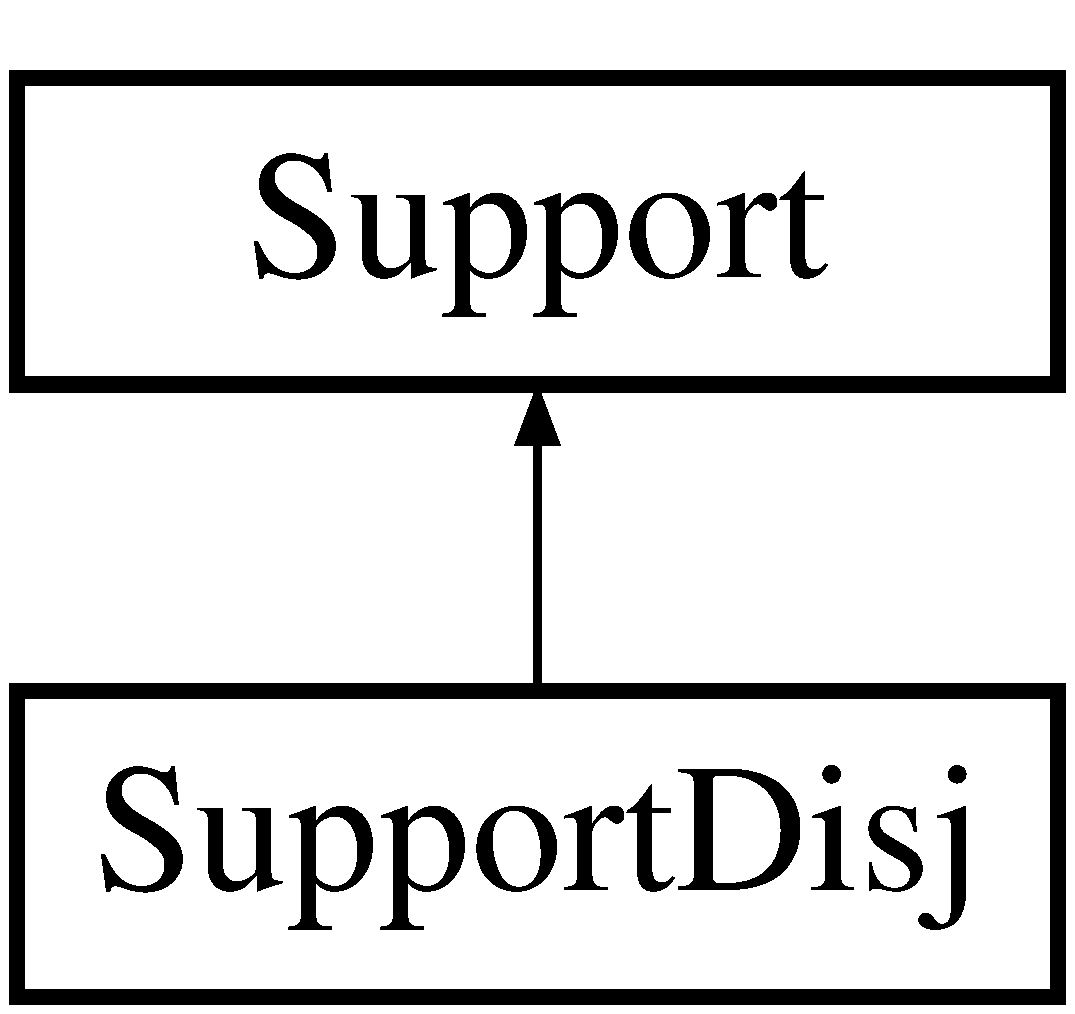
\includegraphics[height=2cm]{class_support}
\end{center}
\end{figure}
\subsection*{Public Member Functions}
\begin{CompactItemize}
\item 
{\bf Support} ()
\begin{CompactList}\small\item\em The constructor by deault, in cunjonction with the operator != to mark that an element is in a node. \item\end{CompactList}\end{CompactItemize}
\subsection*{Public Attributes}
\begin{CompactItemize}
\item 
bool {\bf presence}\label{class_support_1cb32d9c30dfd35099b9118e4234a5c2}

\begin{CompactList}\small\item\em used to not update the support of an itemset already considered \item\end{CompactList}\item 
int {\bf supp}\label{class_support_09e392dcc0f63feaa7b20513cfc8f630}

\begin{CompactList}\small\item\em store the support of the corresponding itemset \item\end{CompactList}\end{CompactItemize}


\subsection{Detailed Description}
Class used to store additional informations in each node, here the support of the corresponding items. 



\subsection{Constructor \& Destructor Documentation}
\index{Support@{Support}!Support@{Support}}
\index{Support@{Support}!Support@{Support}}
\subsubsection{\setlength{\rightskip}{0pt plus 5cm}Support::Support ()\hspace{0.3cm}{\tt  [inline]}}\label{class_support_19bf40018bf3004487c65f7e68c9f65e}


The constructor by deault, in cunjonction with the operator != to mark that an element is in a node. 

An element is in in the node is the {\bf Support}{\rm (p.\,\pageref{class_support})} of the current node is != of {\bf Support()}{\rm (p.\,\pageref{class_support_19bf40018bf3004487c65f7e68c9f65e})}. 

The documentation for this class was generated from the following file:\begin{CompactItemize}
\item 
F:/i\-Zi/problems/frequent/Support.hpp\end{CompactItemize}

\section{Support\-Disj Class Reference}
\label{class_support_disj}\index{SupportDisj@{SupportDisj}}
Class used to store additional informations in each node, here the support and the disjunction of the corresponding items.  


{\tt \#include $<$Support\-Disj.hpp$>$}

Inheritance diagram for Support\-Disj::\begin{figure}[H]
\begin{center}
\leavevmode
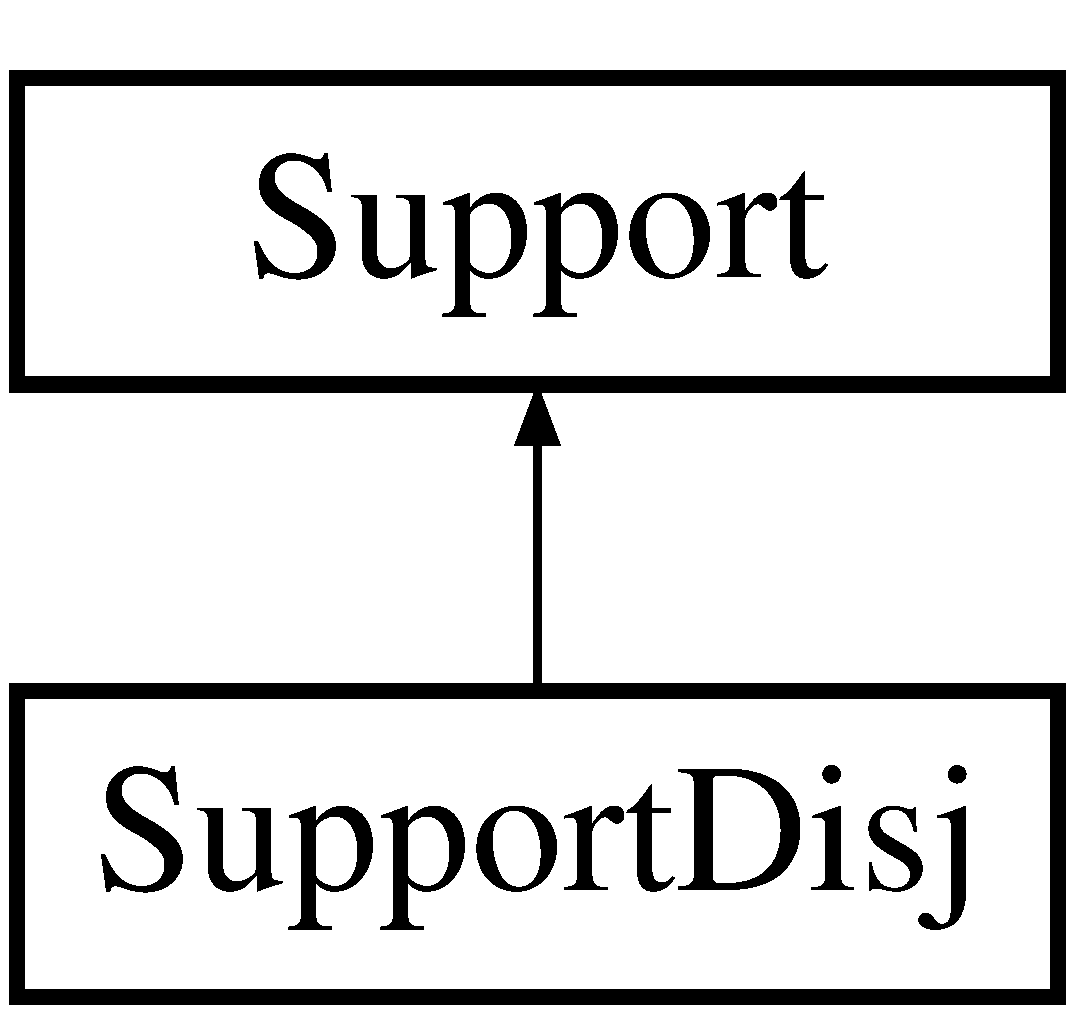
\includegraphics[height=2cm]{class_support_disj}
\end{center}
\end{figure}
\subsection*{Public Member Functions}
\begin{CompactItemize}
\item 
{\bf Support\-Disj} ()
\begin{CompactList}\small\item\em The constructor by deault, in cunjonction with the operator != to mark that an element is in a node. \item\end{CompactList}\end{CompactItemize}
\subsection*{Public Attributes}
\begin{CompactItemize}
\item 
int {\bf disj}\label{class_support_disj_ca1aa0fb612051f04e0ea48051fea157}

\begin{CompactList}\small\item\em store the disjunction of the corresponding itemset \item\end{CompactList}\end{CompactItemize}


\subsection{Detailed Description}
Class used to store additional informations in each node, here the support and the disjunction of the corresponding items. 

The disjunction is the number of transactions intersecting an itemset. 



\subsection{Constructor \& Destructor Documentation}
\index{SupportDisj@{Support\-Disj}!SupportDisj@{SupportDisj}}
\index{SupportDisj@{SupportDisj}!SupportDisj@{Support\-Disj}}
\subsubsection{\setlength{\rightskip}{0pt plus 5cm}Support\-Disj::Support\-Disj ()\hspace{0.3cm}{\tt  [inline]}}\label{class_support_disj_f55cb6b997d16ef0a60148b3091af369}


The constructor by deault, in cunjonction with the operator != to mark that an element is in a node. 

An element is in in the node is the {\bf Support}{\rm (p.\,\pageref{class_support})} of the current node is != of {\bf Support()}{\rm (p.\,\pageref{class_support_19bf40018bf3004487c65f7e68c9f65e})}. 

The documentation for this class was generated from the following file:\begin{CompactItemize}
\item 
F:/i\-Zi/problems/essential/Support\-Disj.hpp\end{CompactItemize}

\section{Tabular\-DBFile Class Reference}
\label{class_tabular_d_b_file}\index{TabularDBFile@{TabularDBFile}}
Read a tabular db and save solution in a file in the FIMI format.  


{\tt \#include $<$Tabular\-DBFile.hxx$>$}

\subsection*{Public Member Functions}
\begin{CompactItemize}
\item 
{\bf Tabular\-DBFile} (char $\ast$in\-File\-Name, {\bf Recode\-To\-Int}$<$ string $>$ $\ast$inrecode\-Tuples=0)
\begin{CompactList}\small\item\em Constructor. \item\end{CompactList}\item 
virtual {\bf $\sim$Tabular\-DBFile} ()
\begin{CompactList}\small\item\em Destructor. \item\end{CompactList}\item 
template$<$class Container\-Bd\-R$>$ {\bf Tabular\-DBFile} \& {\bf operator$>$$>$} (Container\-Bd\-R \&container)
\begin{CompactList}\small\item\em Extract data of the file and insert it in a container. \item\end{CompactList}\item 
template$<$class Container\-Set$>$ {\bf Tabular\-DBFile} \& {\bf operator$<$$<$} (Container\-Set \&container)
\begin{CompactList}\small\item\em Extract data of the container (set of itemsets) and insert it in the file. \item\end{CompactList}\item 
template$<$class Container, class Val$>$ void {\bf push\_\-back} (Container \&set\-Element, Val supp)
\begin{CompactList}\small\item\em Insert an itemset in the file. \item\end{CompactList}\item 
template$<$class Container$>$ void {\bf push\_\-back} (Container \&set\-Element)
\begin{CompactList}\small\item\em Insert an itemset in the file. \item\end{CompactList}\item 
template$<$class Input\-Iterator, class Val$>$ void {\bf push\_\-back} (Input\-Iterator first, Input\-Iterator last, Val supp)
\begin{CompactList}\small\item\em Insert a set of element in the file. \item\end{CompactList}\item 
template$<$class Input\-Iterator, class Val$>$ void {\bf push\_\-back} (Input\-Iterator first, Input\-Iterator last)
\begin{CompactList}\small\item\em Insert a set of element in the file. \item\end{CompactList}\end{CompactItemize}
\subsection*{Public Attributes}
\begin{CompactItemize}
\item 
vector$<$ string $>$ {\bf attributes}\label{class_tabular_d_b_file_a2966fce4c41b8ee7c386c3ff663afd6}

\begin{CompactList}\small\item\em List of all the attributes. \item\end{CompactList}\end{CompactItemize}
\subsection*{Protected Member Functions}
\begin{CompactItemize}
\item 
template$<$class Container\-Tuple$>$ bool {\bf read\-Tuple} (Container\-Tuple \&tuple, {\bf Recode\-To\-Int}$<$ string $>$ $\ast$in\-Recode\-Tuples)
\begin{CompactList}\small\item\em Function reading a tuple in the file. \item\end{CompactList}\item 
template$<$class Container\-Attrib$>$ bool {\bf read\-Attrib} (Container\-Attrib \&attrib)
\begin{CompactList}\small\item\em Function reading the attributes in the file. \item\end{CompactList}\item 
template$<$class Container\-Bd\-T$>$ bool {\bf read} (Container\-Bd\-T \&container, {\bf Recode\-To\-Int}$<$ string $>$ $\ast$in\-Recode\-Tuples=0)
\begin{CompactList}\small\item\em Function reading data in a file and store it in a container. \item\end{CompactList}\item 
template$<$class Iterator, class Val$>$ void {\bf write} (Iterator begin, Iterator end, Val \&supp)
\begin{CompactList}\small\item\em Function write data in a file. \item\end{CompactList}\item 
template$<$class Iterator$>$ void {\bf write} (Iterator begin, Iterator end)
\begin{CompactList}\small\item\em Function write data in a file. \item\end{CompactList}\end{CompactItemize}
\subsection*{Protected Attributes}
\begin{CompactItemize}
\item 
char $\ast$ {\bf file\-Name}\label{class_tabular_d_b_file_d48b2a86d8e34a7ad1f4f5872a6586f0}

\begin{CompactList}\small\item\em name of the file to used \item\end{CompactList}\item 
ifstream {\bf readfile}\label{class_tabular_d_b_file_0a3868d33194605eadb13364e948daf4}

\begin{CompactList}\small\item\em Stream to read in the file. \item\end{CompactList}\item 
ofstream {\bf writefile}\label{class_tabular_d_b_file_b4ed25e63980291bd4dbb9c7ba42fe06}

\begin{CompactList}\small\item\em Stream to write in the file. \item\end{CompactList}\item 
{\bf Recode\-To\-Int}$<$ string $>$ $\ast$ {\bf recode\-Tuples}\label{class_tabular_d_b_file_575cf6ce6322a34660235ca35fe5b6a2}

\begin{CompactList}\small\item\em {\bf Recode}{\rm (p.\,\pageref{class_recode})} the value of the tuples in integer. \item\end{CompactList}\end{CompactItemize}
\subsection*{Classes}
\begin{CompactItemize}
\item 
class {\bf save\-Container\-In\-File}
\begin{CompactList}\small\item\em Functor used to save a solution in the file. \item\end{CompactList}\item 
class {\bf save\-Elem\-In\-File}
\begin{CompactList}\small\item\em Functore used to save an element of a solution in the file. \item\end{CompactList}\end{CompactItemize}


\subsection{Detailed Description}
Read a tabular db and save solution in a file in the FIMI format. 

The input functions of this class read tabular data stored in a file having the following format:\begin{itemize}
\item first line -$>$ list of the attributes separadte by \char`\"{};\char`\"{}\item each line -$>$ one tuple with the values separated by \char`\"{};\char`\"{} The output functions of this class store the solutions in a file in the FIMI format:\item one line -$>$ an element (set of attributes) of the solution\item last value -$>$ the cardinality of the projection of the attributres on the data\end{itemize}


The values int the tuples are recoded to int when stored in memory to occupy less memory 



\subsection{Constructor \& Destructor Documentation}
\index{TabularDBFile@{Tabular\-DBFile}!TabularDBFile@{TabularDBFile}}
\index{TabularDBFile@{TabularDBFile}!TabularDBFile@{Tabular\-DBFile}}
\subsubsection{\setlength{\rightskip}{0pt plus 5cm}Tabular\-DBFile::Tabular\-DBFile (char $\ast$ {\em in\-File\-Name}, {\bf Recode\-To\-Int}$<$ string $>$ $\ast$ {\em inrecode\-Tuples} = {\tt 0})\hspace{0.3cm}{\tt  [inline]}}\label{class_tabular_d_b_file_9dc7164b66cb23bcbf55647d4469e21d}


Constructor. 

The constructor open the file and keep it open until the destruction of the object.

\begin{Desc}
\item[Parameters:]
\begin{description}
\item[{\em in\-File\-Name}]name of the file to access \item[{\em inrecode\-Val\-Attrib}]recode function to recode values of the tuples in int \end{description}
\end{Desc}
\index{TabularDBFile@{Tabular\-DBFile}!~TabularDBFile@{$\sim$TabularDBFile}}
\index{~TabularDBFile@{$\sim$TabularDBFile}!TabularDBFile@{Tabular\-DBFile}}
\subsubsection{\setlength{\rightskip}{0pt plus 5cm}virtual Tabular\-DBFile::$\sim$Tabular\-DBFile ()\hspace{0.3cm}{\tt  [inline, virtual]}}\label{class_tabular_d_b_file_9d038f6432720287f5a5aca26ab8df2e}


Destructor. 

The destructor close the file. 

\subsection{Member Function Documentation}
\index{TabularDBFile@{Tabular\-DBFile}!operator<<@{operator$<$$<$}}
\index{operator<<@{operator$<$$<$}!TabularDBFile@{Tabular\-DBFile}}
\subsubsection{\setlength{\rightskip}{0pt plus 5cm}template$<$class Container\-Set$>$ {\bf Tabular\-DBFile}\& Tabular\-DBFile::operator$<$$<$ (Container\-Set \& {\em container})\hspace{0.3cm}{\tt  [inline]}}\label{class_tabular_d_b_file_e482df0bdff0ce8b734a3a3a2a255aed}


Extract data of the container (set of itemsets) and insert it in the file. 

\begin{Desc}
\item[Parameters:]
\begin{description}
\item[{\em container}]where the data is read (using iterators) and inserted in the file. \end{description}
\end{Desc}
\begin{Desc}
\item[Returns:]$\ast$this. \end{Desc}
\index{TabularDBFile@{Tabular\-DBFile}!operator>>@{operator$>$$>$}}
\index{operator>>@{operator$>$$>$}!TabularDBFile@{Tabular\-DBFile}}
\subsubsection{\setlength{\rightskip}{0pt plus 5cm}template$<$class Container\-Bd\-R$>$ {\bf Tabular\-DBFile}\& Tabular\-DBFile::operator$>$$>$ (Container\-Bd\-R \& {\em container})\hspace{0.3cm}{\tt  [inline]}}\label{class_tabular_d_b_file_6b9390b5d1e89edc3f33f1968a711308}


Extract data of the file and insert it in a container. 

\begin{Desc}
\item[Parameters:]
\begin{description}
\item[{\em container}]where the data read is inserted (must have a push\_\-back function). \end{description}
\end{Desc}
\begin{Desc}
\item[Returns:]$\ast$this. \end{Desc}
\index{TabularDBFile@{Tabular\-DBFile}!push_back@{push\_\-back}}
\index{push_back@{push\_\-back}!TabularDBFile@{Tabular\-DBFile}}
\subsubsection{\setlength{\rightskip}{0pt plus 5cm}template$<$class Input\-Iterator, class Val$>$ void Tabular\-DBFile::push\_\-back (Input\-Iterator {\em first}, Input\-Iterator {\em last})\hspace{0.3cm}{\tt  [inline]}}\label{class_tabular_d_b_file_67bb4415de2083b4f4dc550f60e8bbf1}


Insert a set of element in the file. 

The template parameter represents the input iterators on the integers to insert in the file. \begin{Desc}
\item[Parameters:]
\begin{description}
\item[{\em first}]iterator on the first element. \item[{\em last}]iterator on the element after the last. \end{description}
\end{Desc}
\index{TabularDBFile@{Tabular\-DBFile}!push_back@{push\_\-back}}
\index{push_back@{push\_\-back}!TabularDBFile@{Tabular\-DBFile}}
\subsubsection{\setlength{\rightskip}{0pt plus 5cm}template$<$class Input\-Iterator, class Val$>$ void Tabular\-DBFile::push\_\-back (Input\-Iterator {\em first}, Input\-Iterator {\em last}, Val {\em supp})\hspace{0.3cm}{\tt  [inline]}}\label{class_tabular_d_b_file_3b938a6817ad2b62ece9f6697625252b}


Insert a set of element in the file. 

The template parameter represents the input iterators on the integers to insert in the file. \begin{Desc}
\item[Parameters:]
\begin{description}
\item[{\em first}]iterator on the first element. \item[{\em last}]iterator on the element after the last. \item[{\em supp}]the support of the itemset. \end{description}
\end{Desc}
\index{TabularDBFile@{Tabular\-DBFile}!push_back@{push\_\-back}}
\index{push_back@{push\_\-back}!TabularDBFile@{Tabular\-DBFile}}
\subsubsection{\setlength{\rightskip}{0pt plus 5cm}template$<$class Container$>$ void Tabular\-DBFile::push\_\-back (Container \& {\em set\-Element})\hspace{0.3cm}{\tt  [inline]}}\label{class_tabular_d_b_file_6a6bac3812d26f797c4544beb8437d27}


Insert an itemset in the file. 

This function corresponds to the classic {\bf push\_\-back( )}{\rm (p.\,\pageref{class_tabular_d_b_file_548d79f25d83bd10f9dbfbf542d22b1a})} function od STL container. The template parameter represents a container of integers. \begin{Desc}
\item[Parameters:]
\begin{description}
\item[{\em set\-Element}]the set of element to insert in the file. \end{description}
\end{Desc}
\index{TabularDBFile@{Tabular\-DBFile}!push_back@{push\_\-back}}
\index{push_back@{push\_\-back}!TabularDBFile@{Tabular\-DBFile}}
\subsubsection{\setlength{\rightskip}{0pt plus 5cm}template$<$class Container, class Val$>$ void Tabular\-DBFile::push\_\-back (Container \& {\em set\-Element}, Val {\em supp})\hspace{0.3cm}{\tt  [inline]}}\label{class_tabular_d_b_file_548d79f25d83bd10f9dbfbf542d22b1a}


Insert an itemset in the file. 

This function corresponds to the classic {\bf push\_\-back( )}{\rm (p.\,\pageref{class_tabular_d_b_file_548d79f25d83bd10f9dbfbf542d22b1a})} function od STL container. The template parameter represents a container of integers. \begin{Desc}
\item[Parameters:]
\begin{description}
\item[{\em set\-Element}]the set of element to insert in the file. \item[{\em supp}]the support of the itemset. \end{description}
\end{Desc}
\index{TabularDBFile@{Tabular\-DBFile}!read@{read}}
\index{read@{read}!TabularDBFile@{Tabular\-DBFile}}
\subsubsection{\setlength{\rightskip}{0pt plus 5cm}template$<$class Container\-Bd\-T$>$ bool Tabular\-DBFile::read (Container\-Bd\-T \& {\em container}, {\bf Recode\-To\-Int}$<$ string $>$ $\ast$ {\em in\-Recode\-Tuples} = {\tt 0})\hspace{0.3cm}{\tt  [protected]}}\label{class_tabular_d_b_file_2767edf34b755fb5c3fc672dfdde32f7}


Function reading data in a file and store it in a container. 

\begin{Desc}
\item[Parameters:]
\begin{description}
\item[{\em container}]where the data read is inserted (must have a push\_\-back function). \item[{\em in\-Recode\-Tuples}]to recode the values of the tuples in int \end{description}
\end{Desc}
\begin{Desc}
\item[Returns:]true if data has been read. \end{Desc}
\index{TabularDBFile@{Tabular\-DBFile}!readAttrib@{readAttrib}}
\index{readAttrib@{readAttrib}!TabularDBFile@{Tabular\-DBFile}}
\subsubsection{\setlength{\rightskip}{0pt plus 5cm}template$<$class Container\-Attrib$>$ bool Tabular\-DBFile::read\-Attrib (Container\-Attrib \& {\em attrib})\hspace{0.3cm}{\tt  [protected]}}\label{class_tabular_d_b_file_455cbe09d821a2c4b71766e5338653bd}


Function reading the attributes in the file. 

\begin{Desc}
\item[Parameters:]
\begin{description}
\item[{\em attrib}]stores the attributes (must have a push\_\-back function). \end{description}
\end{Desc}
\begin{Desc}
\item[Returns:]false if end of file \end{Desc}
\index{TabularDBFile@{Tabular\-DBFile}!readTuple@{readTuple}}
\index{readTuple@{readTuple}!TabularDBFile@{Tabular\-DBFile}}
\subsubsection{\setlength{\rightskip}{0pt plus 5cm}template$<$class Container\-Tuple$>$ bool Tabular\-DBFile::read\-Tuple (Container\-Tuple \& {\em tuple}, {\bf Recode\-To\-Int}$<$ string $>$ $\ast$ {\em in\-Recode\-Tuples})\hspace{0.3cm}{\tt  [protected]}}\label{class_tabular_d_b_file_d5a96f52ba726269c868339f1fc585fd}


Function reading a tuple in the file. 

\begin{Desc}
\item[Parameters:]
\begin{description}
\item[{\em tuple}]stores the tuple (must have a push\_\-back function). \item[{\em in\-Recode\-Tuples}]to recode the values of the tuples in int \end{description}
\end{Desc}
\begin{Desc}
\item[Returns:]false if end of file \end{Desc}
\index{TabularDBFile@{Tabular\-DBFile}!write@{write}}
\index{write@{write}!TabularDBFile@{Tabular\-DBFile}}
\subsubsection{\setlength{\rightskip}{0pt plus 5cm}template$<$class Iterator$>$ void Tabular\-DBFile::write (Iterator {\em begin}, Iterator {\em end})\hspace{0.3cm}{\tt  [protected]}}\label{class_tabular_d_b_file_bbf288b62789372257be6f7617fd6ec7}


Function write data in a file. 

\begin{Desc}
\item[Parameters:]
\begin{description}
\item[{\em container}]to read and write in the output. \item[{\em recode}]functor used to recode the data read and store the mapping. \end{description}
\end{Desc}
\index{TabularDBFile@{Tabular\-DBFile}!write@{write}}
\index{write@{write}!TabularDBFile@{Tabular\-DBFile}}
\subsubsection{\setlength{\rightskip}{0pt plus 5cm}template$<$class Iterator, class Val$>$ void Tabular\-DBFile::write (Iterator {\em begin}, Iterator {\em end}, Val \& {\em supp})\hspace{0.3cm}{\tt  [protected]}}\label{class_tabular_d_b_file_b6c2a304ce4003222dd2e89b9d933765}


Function write data in a file. 

\begin{Desc}
\item[Parameters:]
\begin{description}
\item[{\em container}]to read and write in the output. \item[{\em recode}]functor used to recode the data read and store the mapping. \item[{\em supp}]the support of the itemset. \end{description}
\end{Desc}


The documentation for this class was generated from the following file:\begin{CompactItemize}
\item 
F:/i\-Zi/data/file/Tabular\-DBFile.hxx\end{CompactItemize}

\section{Tabular\-DBFile::save\-Container\-In\-File Class Reference}
\label{class_tabular_d_b_file_1_1save_container_in_file}\index{TabularDBFile::saveContainerInFile@{TabularDBFile::saveContainerInFile}}
Functor used to save a solution in the file.  


{\tt \#include $<$Tabular\-DBFile.hxx$>$}



\subsection{Detailed Description}
Functor used to save a solution in the file. 



The documentation for this class was generated from the following file:\begin{CompactItemize}
\item 
F:/i\-Zi/data/file/Tabular\-DBFile.hxx\end{CompactItemize}

\section{Tabular\-DBFile::save\-Elem\-In\-File Class Reference}
\label{class_tabular_d_b_file_1_1save_elem_in_file}\index{TabularDBFile::saveElemInFile@{TabularDBFile::saveElemInFile}}
Functore used to save an element of a solution in the file.  


{\tt \#include $<$Tabular\-DBFile.hxx$>$}



\subsection{Detailed Description}
Functore used to save an element of a solution in the file. 



The documentation for this class was generated from the following file:\begin{CompactItemize}
\item 
F:/i\-Zi/data/file/Tabular\-DBFile.hxx\end{CompactItemize}

\section{Tatree$<$ Sets\-Type $>$ Class Template Reference}
\label{class_tatree}\index{Tatree@{Tatree}}
Template class representing a trie data structure (this is an \char`\"{}interface\char`\"{} of the Tatre\_\-base class).  


{\tt \#include $<$Tatree.hxx$>$}

Inheritance diagram for Tatree$<$ Sets\-Type $>$::\begin{figure}[H]
\begin{center}
\leavevmode
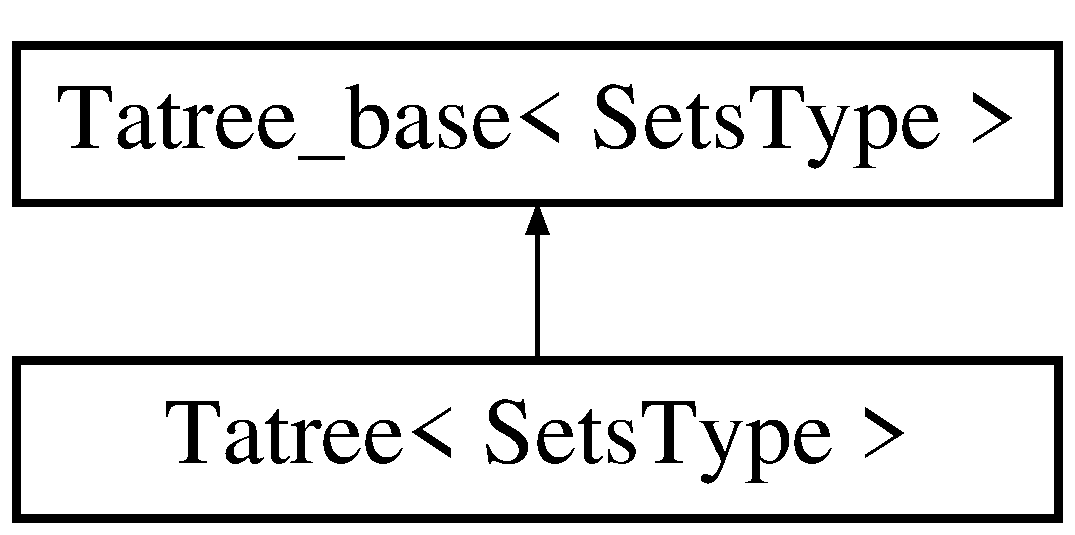
\includegraphics[height=2cm]{class_tatree}
\end{center}
\end{figure}
\subsection*{Public Types}
\begin{CompactItemize}
\item 
typedef {\bf It\-Tatree}$<$ Sets\-Type $>$ {\bf iterator}\label{class_tatree_06094a289a982269a29926e3f22b8356}

\begin{CompactList}\small\item\em Used to have the same syntax tha the STL. \item\end{CompactList}\end{CompactItemize}
\subsection*{Public Member Functions}
\begin{CompactItemize}
\item 
{\bf Tatree} ()\label{class_tatree_7ba7fda13c2987a2840c07164c2d17e6}

\begin{CompactList}\small\item\em Constructor. \item\end{CompactList}\item 
{\bf $\sim$Tatree} ()\label{class_tatree_d54e3fb0fc9525949c010f9290fb97f7}

\begin{CompactList}\small\item\em Destructor. \item\end{CompactList}\item 
{\bf It\-Tatree}$<$ Sets\-Type $>$ {\bf begin} ()\label{class_tatree_383cce0f85279182e9eb5e19015cae0f}

\begin{CompactList}\small\item\em Return an iterator on the first element stored. \item\end{CompactList}\item 
{\bf It\-Tatree}$<$ Sets\-Type $>$ {\bf begin\-Root} ()\label{class_tatree_14ef8d3302fb0d1f520a39b09ba71b65}

\begin{CompactList}\small\item\em Return an iterator on the root node. \item\end{CompactList}\item 
{\bf It\-Tatree}$<$ Sets\-Type $>$ {\bf end} ()\label{class_tatree_7dea4be6a2c8914398d8073189c7e845}

\begin{CompactList}\small\item\em Return an iterator on the element after the last element stored. \item\end{CompactList}\item 
void {\bf print} ()\label{class_tatree_2690856037aef1ae34a711b5f4136069}

\begin{CompactList}\small\item\em Function that print to screen the sets stored in the trie. \item\end{CompactList}\item 
{\bf Tatree\-Node}$<$ Sets\-Type $>$ $\ast$ {\bf get\-Root} ()\label{class_tatree_940b8597e71da99ff8bc673aaad7a53b}

\begin{CompactList}\small\item\em Return the root node. \item\end{CompactList}\item 
void {\bf set\-Recode} ({\bf Recode\-To\-Int}$<$ Sets\-Type $>$ $\ast$inrec)\label{class_tatree_69650ee7743c216a5e4080e2ebaa68a0}

\begin{CompactList}\small\item\em Set the recode functor to the functor passed in parameter. \item\end{CompactList}\item 
{\bf Recode\-To\-Int}$<$ Sets\-Type $>$ $\ast$ {\bf get\-Recode} ()\label{class_tatree_cca02ceb8838b29546f807316b187182}

\begin{CompactList}\small\item\em Get the recode functor. \item\end{CompactList}\end{CompactItemize}
\subsection*{Friends}
\begin{CompactItemize}
\item 
class {\bf It\-Tatree$<$ Sets\-Type $>$}\label{class_tatree_e63ac7816d95fec5ec77b16c2597e4b7}

\end{CompactItemize}


\subsection{Detailed Description}
\subsubsection*{template$<$class Sets\-Type$>$ class Tatree$<$ Sets\-Type $>$}

Template class representing a trie data structure (this is an \char`\"{}interface\char`\"{} of the Tatre\_\-base class). 

This class differs from the mother class {\bf Tatree\_\-base}{\rm (p.\,\pageref{class_tatree__base})} by providing additional methods and the access to a more complete iterator. Using this class, it is possible to explore all the sets stored in trie using the iterators ++. The template parameter is the type of the element stored in the trie. 



The documentation for this class was generated from the following file:\begin{CompactItemize}
\item 
F:/i\-Zi/data\-Structures/trie/Tatree.hxx\end{CompactItemize}

\section{Tatree\_\-base$<$ Sets\-Type $>$ Class Template Reference}
\label{class_tatree__base}\index{Tatree_base@{Tatree\_\-base}}
Template class representing a trie data structure.  


{\tt \#include $<$Tatree\_\-base.hxx$>$}

Inheritance diagram for Tatree\_\-base$<$ Sets\-Type $>$::\begin{figure}[H]
\begin{center}
\leavevmode
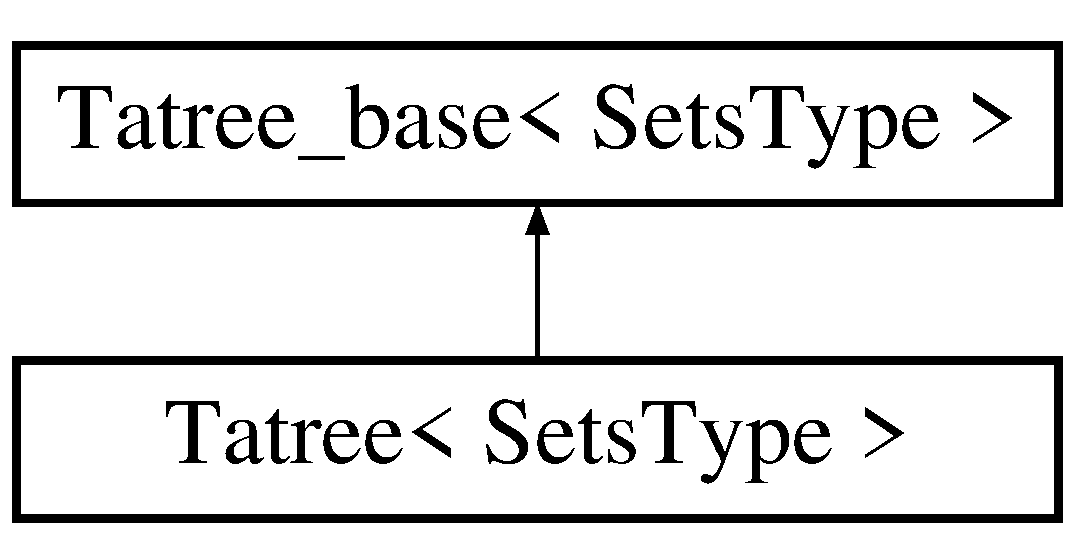
\includegraphics[height=2cm]{class_tatree__base}
\end{center}
\end{figure}
\subsection*{Public Types}
\begin{CompactItemize}
\item 
typedef {\bf It\-Tatree\_\-base}$<$ Sets\-Type $>$ {\bf iterator}\label{class_tatree__base_6f81c0610c9b60a3067eacc19fbe0190}

\begin{CompactList}\small\item\em Used to have the same syntax tha the STL. \item\end{CompactList}\end{CompactItemize}
\subsection*{Public Member Functions}
\begin{CompactItemize}
\item 
{\bf Tatree\_\-base} ()\label{class_tatree__base_c8206aefa793dc39fefa7d5112ac17a1}

\begin{CompactList}\small\item\em Constructor. \item\end{CompactList}\item 
{\bf $\sim$Tatree\_\-base} ()\label{class_tatree__base_0c831209dadbd62486cfcfc39864b5e7}

\begin{CompactList}\small\item\em Destructor. \item\end{CompactList}\item 
template$<$class Container$>$ void {\bf push\_\-back} (Container \&set\-Element, int nb=1)
\begin{CompactList}\small\item\em Push back a set of element in the trie. \item\end{CompactList}\item 
template$<$class Input\-Iterator$>$ void {\bf push\_\-back} (Input\-Iterator \&first, Input\-Iterator \&last, int nb=1)
\begin{CompactList}\small\item\em Push back a set of element in the trie. \item\end{CompactList}\item 
int {\bf size} ()\label{class_tatree__base_7b328d694667e2361991e7e39a911311}

\begin{CompactList}\small\item\em Function that returns the number of sets in the trie. \item\end{CompactList}\item 
{\bf It\-Tatree\_\-base}$<$ Sets\-Type $>$ {\bf begin} ()\label{class_tatree__base_5ac683d9ee2312f85017264dac63ff90}

\begin{CompactList}\small\item\em Return an iterator on the root node. \item\end{CompactList}\item 
{\bf It\-Tatree\_\-base}$<$ Sets\-Type $>$ {\bf begin\-Root} ()\label{class_tatree__base_b14eebc51ea7fc7afbfa3b1092cf093f}

\begin{CompactList}\small\item\em Return an iterator on the root node. \item\end{CompactList}\item 
{\bf It\-Tatree\_\-base}$<$ Sets\-Type $>$ {\bf end} ()\label{class_tatree__base_7021c1f8a67b2aea0d0f7675eb4a1167}

\begin{CompactList}\small\item\em Return an iterator on the element after the last element stored. \item\end{CompactList}\end{CompactItemize}
\subsection*{Protected Attributes}
\begin{CompactItemize}
\item 
{\bf Tatree\-Node}$<$ Sets\-Type $>$ $\ast$ {\bf root}\label{class_tatree__base_41ed3923edf2e25c6f9584a925e42291}

\begin{CompactList}\small\item\em Root node of the trie. \item\end{CompactList}\item 
{\bf Recode\-To\-Int}$<$ Sets\-Type $>$ $\ast$ {\bf recode}\label{class_tatree__base_4120099089ee2c29dd671e16aa7f5b3e}

\begin{CompactList}\small\item\em Functor used to recode and order elements. \item\end{CompactList}\item 
int {\bf nb\-Sets}\label{class_tatree__base_8a743634952a09c67867d0ed62c2b253}

\begin{CompactList}\small\item\em number of elements in the trie \item\end{CompactList}\end{CompactItemize}
\subsection*{Friends}
\begin{CompactItemize}
\item 
class {\bf It\-Tatree\_\-base$<$ Sets\-Type $>$}\label{class_tatree__base_1ce67181fc35f375e5115a7dfb1f0b3c}

\end{CompactItemize}


\subsection{Detailed Description}
\subsubsection*{template$<$class Sets\-Type$>$ class Tatree\_\-base$<$ Sets\-Type $>$}

Template class representing a trie data structure. 

The operations on a {\bf Tatree\_\-base}{\rm (p.\,\pageref{class_tatree__base})} are limited. For example, we cannot directly acces to the transactions by using ++ and $\ast$. The advantage of that type of structure is that it is lighter than one with more operations. Consequently code dedicated to such class will be more efficient.

The template parameter is the type of the element stored in the trie. 



\subsection{Member Function Documentation}
\index{Tatree_base@{Tatree\_\-base}!push_back@{push\_\-back}}
\index{push_back@{push\_\-back}!Tatree_base@{Tatree\_\-base}}
\subsubsection{\setlength{\rightskip}{0pt plus 5cm}template$<$class Sets\-Type$>$ template$<$class Input\-Iterator$>$ void {\bf Tatree\_\-base}$<$ Sets\-Type $>$::push\_\-back (Input\-Iterator \& {\em first}, Input\-Iterator \& {\em last}, int {\em nb} = {\tt 1})\hspace{0.3cm}{\tt  [inline]}}\label{class_tatree__base_6d855d39b3bdf83c4c759190d763e20a}


Push back a set of element in the trie. 

The template parameter represents the input iterators on the elements to insert in the trie. \begin{Desc}
\item[Parameters:]
\begin{description}
\item[{\em first}]iterator on the first element \item[{\em last}]iterator on the element after the last \item[{\em nb}]the number of times the set is inserted \end{description}
\end{Desc}
\index{Tatree_base@{Tatree\_\-base}!push_back@{push\_\-back}}
\index{push_back@{push\_\-back}!Tatree_base@{Tatree\_\-base}}
\subsubsection{\setlength{\rightskip}{0pt plus 5cm}template$<$class Sets\-Type$>$ template$<$class Container$>$ void {\bf Tatree\_\-base}$<$ Sets\-Type $>$::push\_\-back (Container \& {\em set\-Element}, int {\em nb} = {\tt 1})\hspace{0.3cm}{\tt  [inline]}}\label{class_tatree__base_66e0c0d2fa534d9cf53a9b5fe732eb79}


Push back a set of element in the trie. 

This function corresponds to the classic {\bf push\_\-back( )}{\rm (p.\,\pageref{class_tatree__base_66e0c0d2fa534d9cf53a9b5fe732eb79})} function od STL container. The template parameter represents a container of element of type Sets\-Type. \begin{Desc}
\item[Parameters:]
\begin{description}
\item[{\em set\-Element}]the set of element to insert in the trie \item[{\em nb}]the number of times the set is inserted \end{description}
\end{Desc}


The documentation for this class was generated from the following file:\begin{CompactItemize}
\item 
F:/i\-Zi/data\-Structures/trie/Tatree\_\-base.hxx\end{CompactItemize}

\section{Tatree\-Node$<$ Sets\-Type $>$ Class Template Reference}
\label{class_tatree_node}\index{TatreeNode@{TatreeNode}}
Template class representing a node of a trie data structure.  


{\tt \#include $<$Tatree\-Node.hxx$>$}

\subsection*{Public Member Functions}
\begin{CompactItemize}
\item 
{\bf Tatree\-Node} (int incnt=0)\label{class_tatree_node_c1d3bb5eb337c148e101f300efa0719d}

\begin{CompactList}\small\item\em Constructor. \item\end{CompactList}\item 
{\bf $\sim$Tatree\-Node} ()\label{class_tatree_node_f6971420a5eedc158eafbfca2115cb17}

\begin{CompactList}\small\item\em Destructor. \item\end{CompactList}\item 
template$<$class Container$>$ void {\bf push\_\-back} (Container \&set\-Element, int nb=0)
\begin{CompactList}\small\item\em Push back a set of element from this node. \item\end{CompactList}\item 
template$<$class Input\-Iterator$>$ void {\bf push\_\-back} (Input\-Iterator \&first, Input\-Iterator \&last, int nb=0)
\begin{CompactList}\small\item\em Push back a set of element from this node. \item\end{CompactList}\item 
int {\bf number} ()\label{class_tatree_node_09aa679da0752a8f7881fb1d43e492af}

\begin{CompactList}\small\item\em Return the number of occurence of the set stored in the previous nodes. \item\end{CompactList}\item 
map\-TTatree \& {\bf childs} ()\label{class_tatree_node_77117d3078d2d307be2e7ef7e3bdc939}

\begin{CompactList}\small\item\em Return the nodes and their child nodes. \item\end{CompactList}\end{CompactItemize}
\subsection*{Protected Attributes}
\begin{CompactItemize}
\item 
int {\bf cnt}\label{class_tatree_node_b0d8de188c9e2935d0983836de4f24f0}

\begin{CompactList}\small\item\em Numbers of sets stored in the previous nodes. \item\end{CompactList}\item 
int {\bf max}\label{class_tatree_node_5601ac158f5ef263bf987361dabce640}

\begin{CompactList}\small\item\em Size of the largest set. \item\end{CompactList}\item 
map\-TTatree {\bf items}\label{class_tatree_node_c164a7fff2a31d23da5305aa85c8c6eb}

\begin{CompactList}\small\item\em Items in the node and corresponding childs nodes. \item\end{CompactList}\end{CompactItemize}
\subsection*{Friends}
\begin{CompactItemize}
\item 
class {\bf It\-Tatree\_\-base$<$ Sets\-Type $>$}\label{class_tatree_node_1ce67181fc35f375e5115a7dfb1f0b3c}

\item 
class {\bf Tatree\_\-base$<$ Sets\-Type $>$}\label{class_tatree_node_4d067db2add706706c659a83c3cbcf41}

\item 
class {\bf It\-Tatree$<$ Sets\-Type $>$}\label{class_tatree_node_e63ac7816d95fec5ec77b16c2597e4b7}

\item 
class {\bf Tatree$<$ Sets\-Type $>$}\label{class_tatree_node_d092d4c79b0d187f36b3f75573889423}

\end{CompactItemize}
\subsection*{Classes}
\begin{CompactItemize}
\item 
class {\bf insert\-Node}
\begin{CompactList}\small\item\em functor used to add an element in a node \item\end{CompactList}\end{CompactItemize}


\subsection{Detailed Description}
\subsubsection*{template$<$class Sets\-Type$>$ class Tatree\-Node$<$ Sets\-Type $>$}

Template class representing a node of a trie data structure. 

This class represents a node of a trie data structure storing sets of values. The element in the node are stored in lexicographic order.

The template parameter is the type of the element stored in the trie. 



\subsection{Member Function Documentation}
\index{TatreeNode@{Tatree\-Node}!push_back@{push\_\-back}}
\index{push_back@{push\_\-back}!TatreeNode@{Tatree\-Node}}
\subsubsection{\setlength{\rightskip}{0pt plus 5cm}template$<$class Sets\-Type$>$ template$<$class Input\-Iterator$>$ void {\bf Tatree\-Node}$<$ Sets\-Type $>$::push\_\-back (Input\-Iterator \& {\em first}, Input\-Iterator \& {\em last}, int {\em nb} = {\tt 0})\hspace{0.3cm}{\tt  [inline]}}\label{class_tatree_node_b54221d3b995b8d20098f0e7325e1f79}


Push back a set of element from this node. 

The template parameter represents the input iterators on the elements to insert. \begin{Desc}
\item[Parameters:]
\begin{description}
\item[{\em first}]iterator on the first element \item[{\em last}]iterator on the element after the last \item[{\em nb}]the number of times the set is inserted \end{description}
\end{Desc}
\index{TatreeNode@{Tatree\-Node}!push_back@{push\_\-back}}
\index{push_back@{push\_\-back}!TatreeNode@{Tatree\-Node}}
\subsubsection{\setlength{\rightskip}{0pt plus 5cm}template$<$class Sets\-Type$>$ template$<$class Container$>$ void {\bf Tatree\-Node}$<$ Sets\-Type $>$::push\_\-back (Container \& {\em set\-Element}, int {\em nb} = {\tt 0})\hspace{0.3cm}{\tt  [inline]}}\label{class_tatree_node_b8ab38f4a513579212225b8a5bf647f9}


Push back a set of element from this node. 

This function corresponds to the classic {\bf push\_\-back( )}{\rm (p.\,\pageref{class_tatree_node_b8ab38f4a513579212225b8a5bf647f9})} function od STL container. The template parameter represents a container of element of type Sets\-Type. \begin{Desc}
\item[Parameters:]
\begin{description}
\item[{\em set\-Element}]the set of element to insert. \item[{\em nb}]the number of times the set is inserted. \end{description}
\end{Desc}


The documentation for this class was generated from the following file:\begin{CompactItemize}
\item 
F:/i\-Zi/data\-Structures/trie/Tatree\-Node.hxx\end{CompactItemize}

\section{Tatree\-Node$<$ Sets\-Type $>$::insert\-Node Class Reference}
\label{class_tatree_node_1_1insert_node}\index{TatreeNode::insertNode@{TatreeNode::insertNode}}
functor used to add an element in a node  


{\tt \#include $<$Tatree\-Node.hxx$>$}

\subsection*{Public Member Functions}
\begin{CompactItemize}
\item 
{\bf insert\-Node} ({\bf Tatree\-Node}$<$ Sets\-Type $>$ $\ast$in\-Node, int in\-Nb=0)\label{class_tatree_node_1_1insert_node_dc6f2d230c41ebca07df5988eb9c53b3}

\begin{CompactList}\small\item\em number of sets to insert \item\end{CompactList}\end{CompactItemize}


\subsection{Detailed Description}
\subsubsection*{template$<$class Sets\-Type$>$ class Tatree\-Node$<$ Sets\-Type $>$::insert\-Node}

functor used to add an element in a node 

This functor is used in th {\bf push\_\-back()}{\rm (p.\,\pageref{class_tatree_node_b8ab38f4a513579212225b8a5bf647f9})} function. \begin{Desc}
\item[See also:]{\bf push\_\-back()}{\rm (p.\,\pageref{class_tatree_node_b8ab38f4a513579212225b8a5bf647f9})} \end{Desc}




The documentation for this class was generated from the following file:\begin{CompactItemize}
\item 
F:/i\-Zi/data\-Structures/trie/Tatree\-Node.hxx\end{CompactItemize}

\section{Test\-Subsets$<$ Sets\-Type $>$ Class Template Reference}
\label{class_test_subsets}\index{TestSubsets@{TestSubsets}}
Functor testing all the k-1 subsets of the itemset passed in parameter wrt to a binary predicate.  


{\tt \#include $<$Test\-Subsets.hxx$>$}



\subsection{Detailed Description}
\subsubsection*{template$<$class Sets\-Type$>$ class Test\-Subsets$<$ Sets\-Type $>$}

Functor testing all the k-1 subsets of the itemset passed in parameter wrt to a binary predicate. 



The documentation for this class was generated from the following file:\begin{CompactItemize}
\item 
F:/i\-Zi/util/Test\-Subsets.hxx\end{CompactItemize}

\section{Transform\-Element$<$ Transform\-Set, Sets\-Type, Word\-To\-Set, Word $>$ Class Template Reference}
\label{class_transform_element}\index{TransformElement@{TransformElement}}
Functor used to transform elements of the langugage.  


{\tt \#include $<$Transform\-Element.hxx$>$}

\subsection*{Public Member Functions}
\begin{CompactItemize}
\item 
{\bf Transform\-Element} (Word\-To\-Set $\ast$inwordtoset, Transform\-Set $\ast$intransformset)\label{class_transform_element_719623f74be497a502346662d13cf4ef}

\begin{CompactList}\small\item\em Constructor. \item\end{CompactList}\item 
template$<$class Iterator\-Word$>$ vector$<$ Sets\-Type $>$ $\ast$ {\bf operator()} (Iterator\-Word w)
\begin{CompactList}\small\item\em Operator applying the transformations functions. \item\end{CompactList}\item 
template$<$class Iterator\-Set$>$ Word $\ast$ {\bf inverse} (Iterator\-Set s)
\begin{CompactList}\small\item\em Method returning original element. \item\end{CompactList}\end{CompactItemize}
\subsection*{Public Attributes}
\begin{CompactItemize}
\item 
Word\-To\-Set $\ast$ {\bf wordtoset}\label{class_transform_element_2b9cd853fe9bbf27160693c29b7d666c}

\begin{CompactList}\small\item\em Functor to transform a word into a set. \item\end{CompactList}\item 
Transform\-Set $\ast$ {\bf transformset}\label{class_transform_element_1c5bcca50f2850e15b2066da3b7b4305}

\begin{CompactList}\small\item\em Functor to transform a set. \item\end{CompactList}\end{CompactItemize}


\subsection{Detailed Description}
\subsubsection*{template$<$class Transform\-Set, class Sets\-Type, class Word\-To\-Set, class Word = vector$<$ Sets\-Type $>$$>$ class Transform\-Element$<$ Transform\-Set, Sets\-Type, Word\-To\-Set, Word $>$}

Functor used to transform elements of the langugage. 

This class could be used to transform words of the language into sets and to eventually transform the sets. The template parameter Word\-To\-Set is the type of the function that transforms the language in sets. The template parameter Transform\-Set is the type of the function that transforms the sets. The template parameter Sets\-Type is the type of the sets elements. 



\subsection{Member Function Documentation}
\index{TransformElement@{Transform\-Element}!inverse@{inverse}}
\index{inverse@{inverse}!TransformElement@{Transform\-Element}}
\subsubsection{\setlength{\rightskip}{0pt plus 5cm}template$<$class Transform\-Set, class Sets\-Type, class Word\-To\-Set, class Word = vector$<$ Sets\-Type $>$$>$ template$<$class Iterator\-Set$>$ Word$\ast$ {\bf Transform\-Element}$<$ Transform\-Set, Sets\-Type, Word\-To\-Set, Word $>$::inverse (Iterator\-Set {\em s})\hspace{0.3cm}{\tt  [inline]}}\label{class_transform_element_c7fc099ae3e5f139a9539e82788823f3}


Method returning original element. 

\begin{Desc}
\item[Parameters:]
\begin{description}
\item[{\em s}]set to transform in the origianl word \end{description}
\end{Desc}
\index{TransformElement@{Transform\-Element}!operator()@{operator()}}
\index{operator()@{operator()}!TransformElement@{Transform\-Element}}
\subsubsection{\setlength{\rightskip}{0pt plus 5cm}template$<$class Transform\-Set, class Sets\-Type, class Word\-To\-Set, class Word = vector$<$ Sets\-Type $>$$>$ template$<$class Iterator\-Word$>$ vector$<$Sets\-Type$>$$\ast$ {\bf Transform\-Element}$<$ Transform\-Set, Sets\-Type, Word\-To\-Set, Word $>$::operator() (Iterator\-Word {\em w})\hspace{0.3cm}{\tt  [inline]}}\label{class_transform_element_cfa1c9f1f11a8400bf8654b4bc03eb06}


Operator applying the transformations functions. 

\begin{Desc}
\item[Parameters:]
\begin{description}
\item[{\em w}]word to transform into set \end{description}
\end{Desc}


The documentation for this class was generated from the following file:\begin{CompactItemize}
\item 
F:/i\-Zi/algorithms/Transform\-Element.hxx\end{CompactItemize}

\section{Unary\-IND Class Reference}
\label{class_unary_i_n_d}\index{UnaryIND@{UnaryIND}}
Class representing the inclusion between two attributes.  


{\tt \#include $<$IND.hpp$>$}

\subsection*{Public Member Functions}
\begin{CompactItemize}
\item 
{\bf Unary\-IND} ()\label{class_unary_i_n_d_94f0ab52803c2a3695768e55dcfd9b8a}

\begin{CompactList}\small\item\em Default constructor. \item\end{CompactList}\item 
{\bf Unary\-IND} (string inleft, string inright)\label{class_unary_i_n_d_b37ed0b8cf369be738c14aadeb343656}

\begin{CompactList}\small\item\em Constructor. \item\end{CompactList}\item 
{\bf Unary\-IND} (const {\bf Unary\-IND} \&indi)\label{class_unary_i_n_d_ca18f4ff42a4411b25f050d8086b834d}

\begin{CompactList}\small\item\em Copy constructor. \item\end{CompactList}\item 
{\bf Unary\-IND} \& {\bf operator=} (const {\bf Unary\-IND} \&indi)\label{class_unary_i_n_d_117105999c93d625df53fbba0aa87a97}

\begin{CompactList}\small\item\em Operator = overloading. \item\end{CompactList}\item 
bool {\bf operator==} (const {\bf Unary\-IND} \&indi) const \label{class_unary_i_n_d_915b2dccf5c5c1af8eb4d50736f13df9}

\begin{CompactList}\small\item\em Equality operator overloading. \item\end{CompactList}\item 
bool {\bf operator!=} (const {\bf Unary\-IND} \&indi) const \label{class_unary_i_n_d_b1eb4d645b77166af3484258a5e64a9d}

\begin{CompactList}\small\item\em Inequality operator overloading. \item\end{CompactList}\item 
bool {\bf operator$<$} (const {\bf Unary\-IND} \&indi) const \label{class_unary_i_n_d_fb5226bfb2f58c322336979158684413}

\begin{CompactList}\small\item\em Less than operator overloading. \item\end{CompactList}\end{CompactItemize}
\subsection*{Public Attributes}
\begin{CompactItemize}
\item 
string {\bf right}\label{class_unary_i_n_d_2a3c36d6618017a28d992f80e87eba57}

\begin{CompactList}\small\item\em right side of the inclusion \item\end{CompactList}\end{CompactItemize}


\subsection{Detailed Description}
Class representing the inclusion between two attributes. 



The documentation for this class was generated from the following file:\begin{CompactItemize}
\item 
F:/i\-Zi/problems/DI/IND.hpp\end{CompactItemize}

\printindex
\end{document}
